\clearpage
\newpage
\section{Systematic Uncertainties}
\label{sec:bssystematics}
Various systematics are taken into account, both 
on our expected signal and background estimate. Some systematic uncertainties will affect only the normalization of certain event rates, 
and are reported as overall normalization uncertainties. Other systematics affect the shapes of the reconstructed signal or backgrounds, as well as their normalization.  

The uncertainty sources of jet energy scale, trigger, jet energy resolution, jet angular resolution,  parton distribution functions, pileup, and $\mathrm{Q^2}$ scale are considered 
and we use the prescriptions outlined in Section~\ref{sec:systematics}.  Figure \ref{figs:bsttbarJES} shows the systematic shapes from the 
jet energy scale on the $\ttbar$ distribution.  Jet energy scale variation on signal MC is shown in Figure \ref{figs:bssignalJES} for 1200$~\GeV$,
 1300$~\GeV$, and 1400$~\GeV$ mass points.  The effects of this on the $\ttbar$ 
distribution due to the trigger systematic variation is shown in Figure \ref{figs:bsttbartrig}. The trigger weighting systematic uncertainty on signal MC is 
shown in Figure \ref{figs:bssignaltrig} for 1200$~\GeV$,
 1300$~\GeV$, and 1400$~\GeV$ mass points.  The uncertainty is low in the mass range of interest for limit setting.  
The jet energy resolution variation in $\ttbar$ MC can be seen in Figure \ref{figs:bsttbarJER}.  Jet energy resolution variation on signal MC 
is shown in Figure \ref{figs:bssignalJER} for 1200$~\GeV$, 1300$~\GeV$, and 1400$~\GeV$ mass points.  
The jet angular resolution variation in $\ttbar$ MC can be seen in Figure \ref{figs:bsttbarJAR} . Jet angular resolution 
variation on signal MC is shown in Figure \ref{figs:bssignalJAR} for 1200$~\GeV$, 1300$~\GeV$, and 1400$~\GeV$ mass points.  
The effect is very small and thus not considered in setting limits.  PDF variation on signal MC is shown in Figure \ref{figs:bssignalPDF} for 1200$~\GeV$,
 1300$~\GeV$, and 1400$~\GeV$ mass points.  PDF variation on $\ttbar$ MC is shown in Figure \ref{figs:bsttbarPDF}.  
The effect is very small and thus not considered in setting limits.  The pileup reweighting uncertainty variation for signal  
can be seen in figure \ref{figs:bssignalPU}.  The effect is very small and thus not considered in setting limits.  
The $\mathrm{Q^2}$ scale uncertainty can be seen in Figure \ref{figs:bsq2scale}.


\begin{figure}[htcb]
\begin{center}
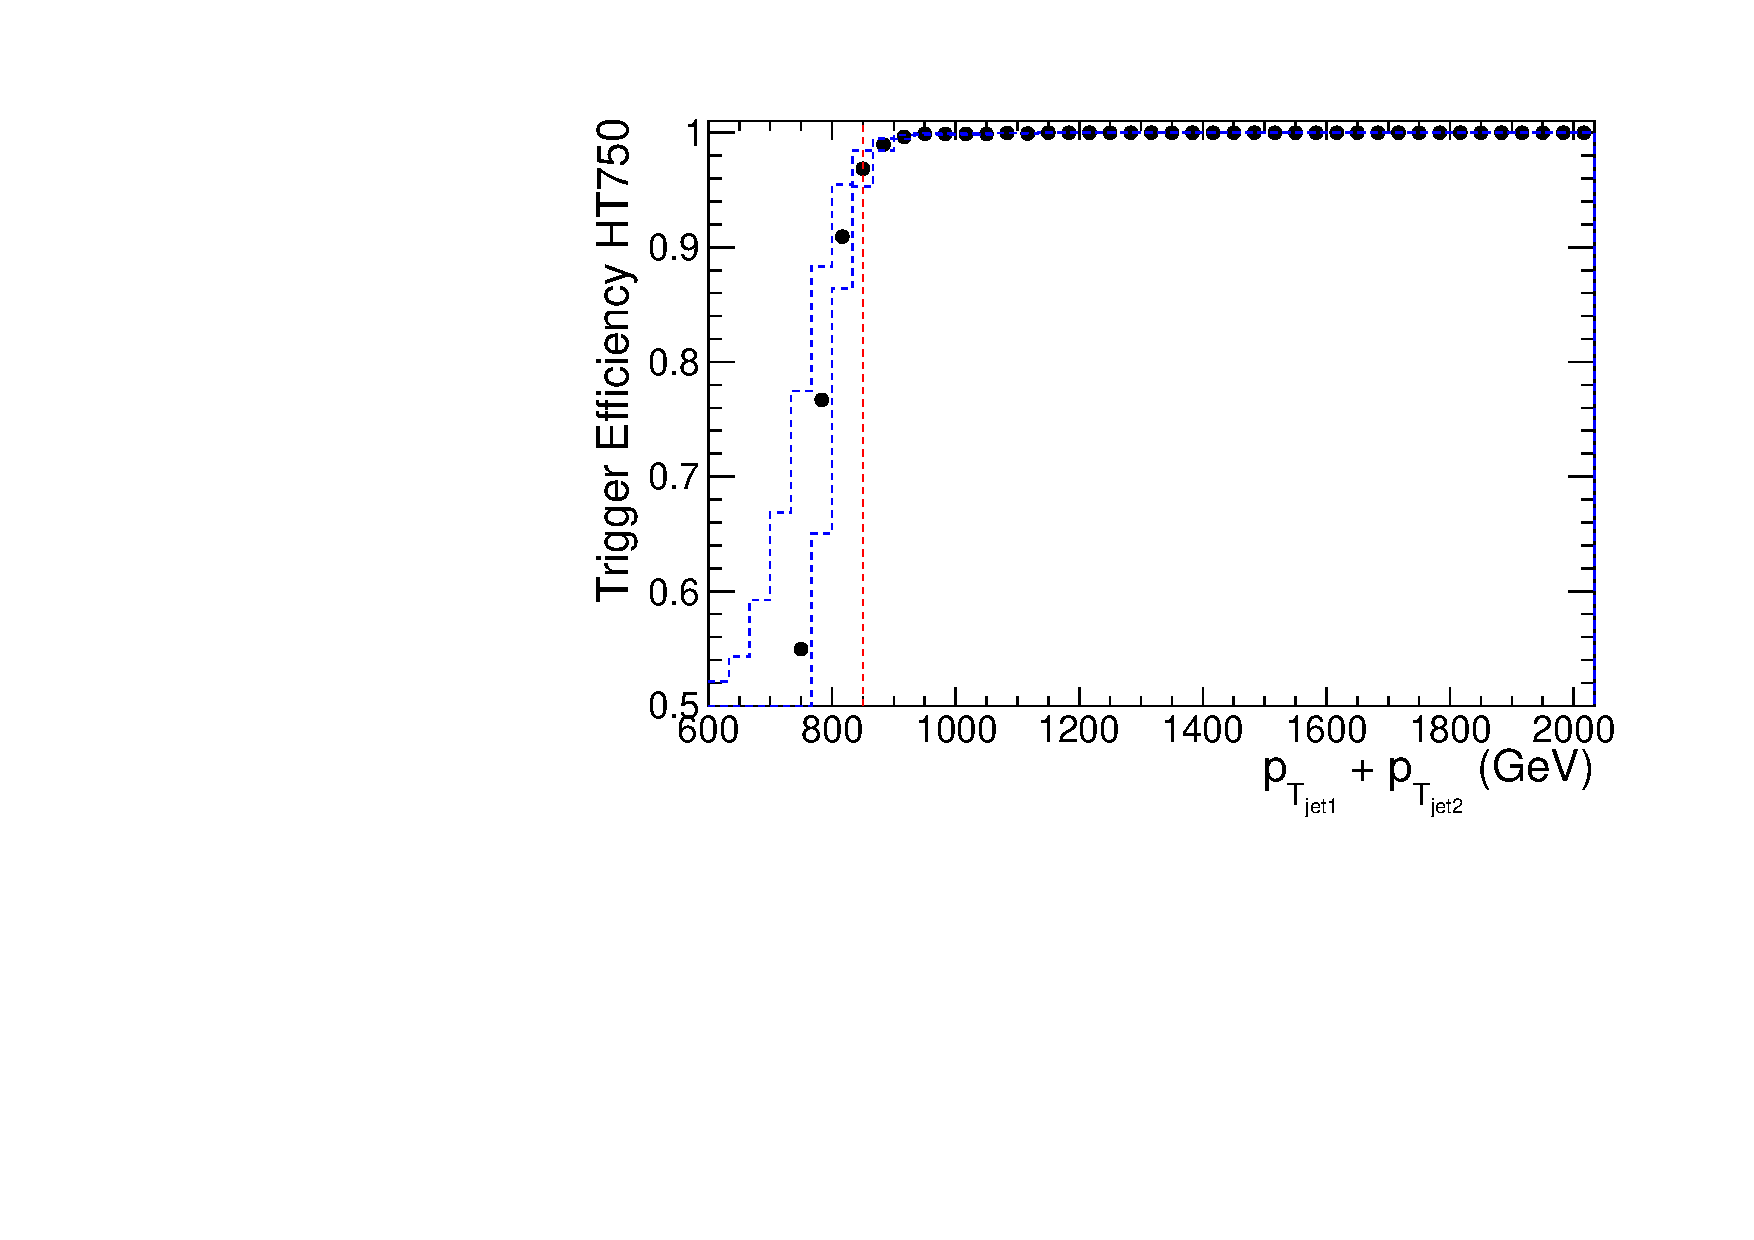
\includegraphics[width=0.7\textwidth]{AN-14-049/figs/Trigger_Comparison_Htdijet_dataonly_withsyst}
\caption{
Trigger efficiency systematic variation. 
}
\label{figs:bsteffsys}
\end{center}
\end{figure}


\begin{figure}[htcb]
\begin{center}
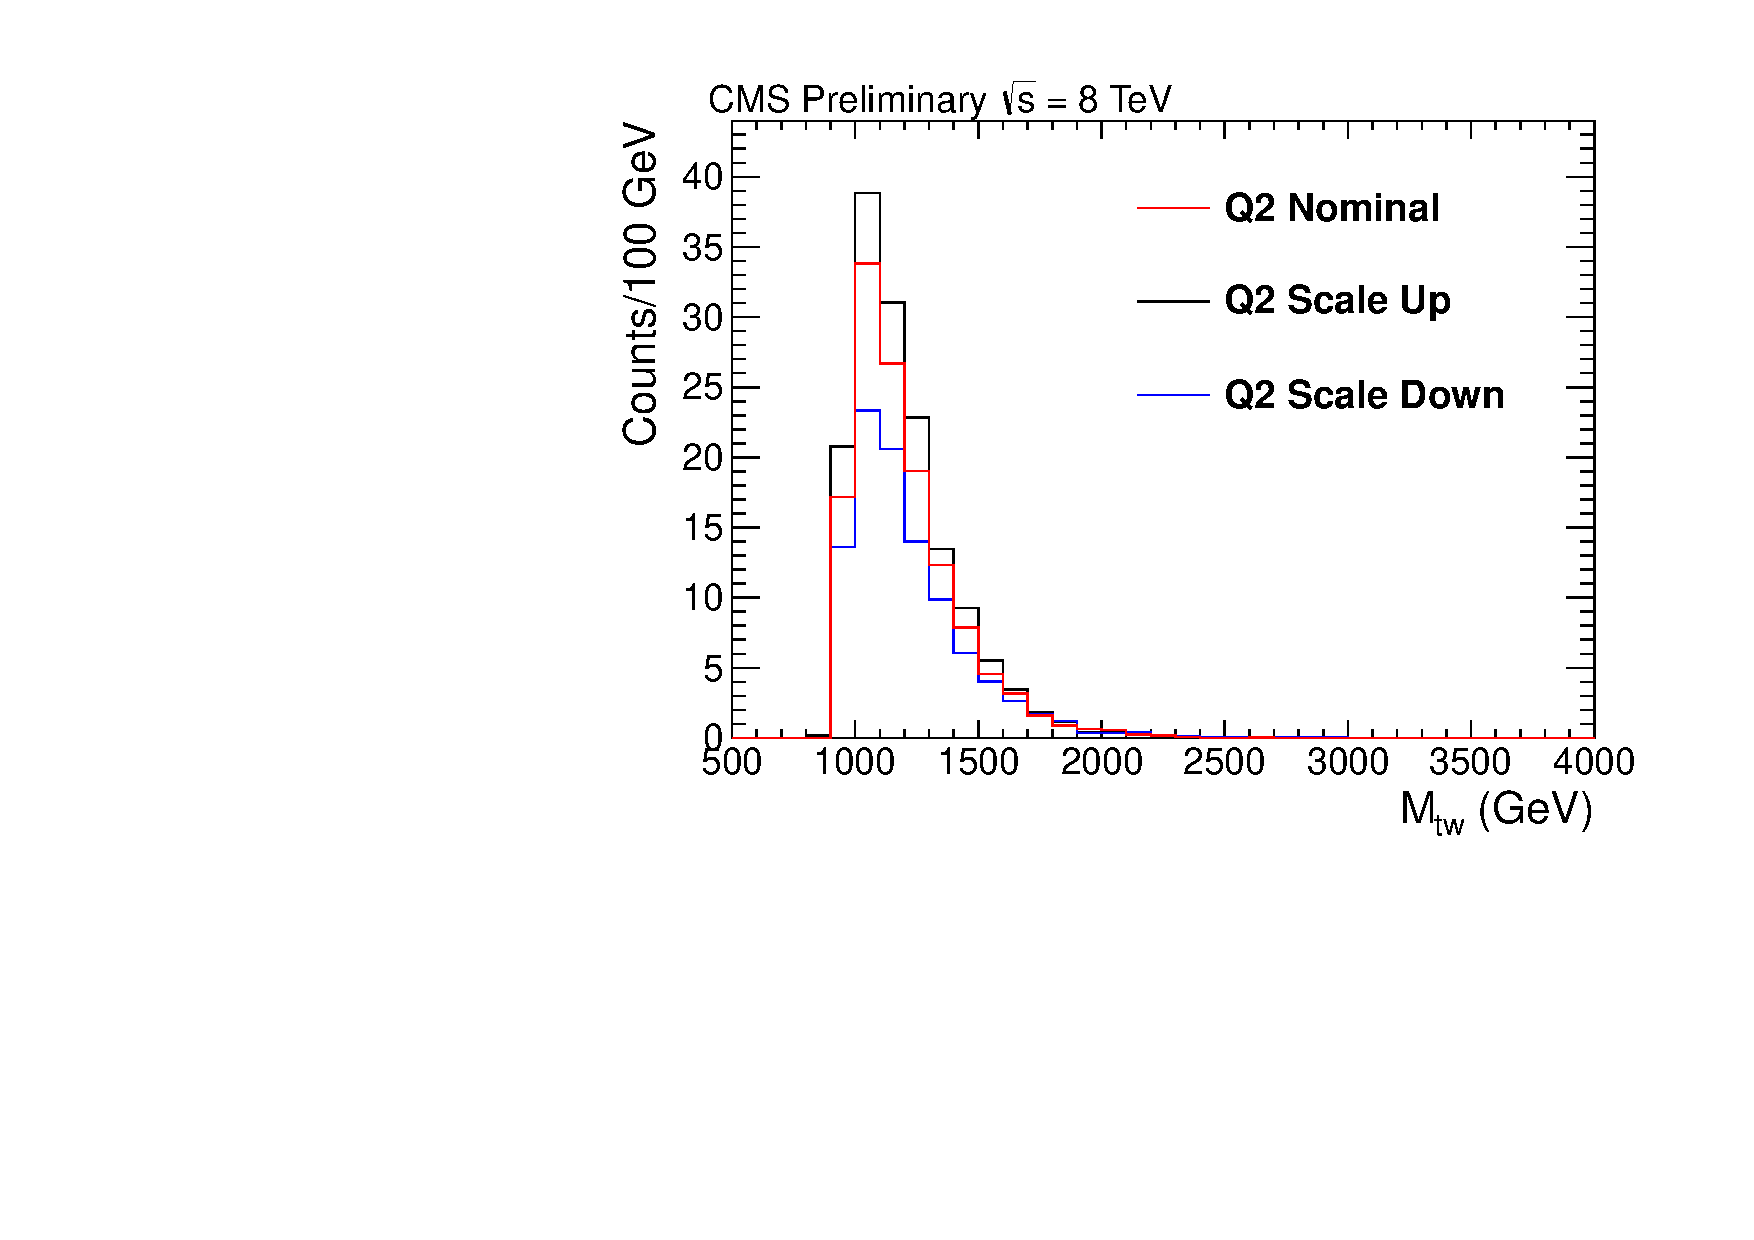
\includegraphics[width=0.7\textwidth]{AN-14-049/figs/TTbar_Q2Scale}
\caption{
$\mathrm{Q^2}$ systematic variation for $\ttbar$ MC 
}
\label{figs:bsq2scale}
\end{center}
\end{figure}


\subsection{Normalization Uncertainties}
As mentioned in Section \ref{sec:bsttbarsideband}, the uncertainty on the overall normalization scale factor used for $\ttbar$ is extracted from data and is 22\%.   

We must apply a 13\% uncertainty on the top tagging scale factor described in Section \ref{sec:subjetSF} 
to signal MC events due to uncertainty in the difference in subjet efficiency from data to MC.

The cross-section uncertainty of 20\%,15\%,30\% applies single-top quark background tW,t,and s channels respectively are applied.

We also include a 2.6\% uncertainty in the luminosity for the signal MC \cite{CMS-PAS-LUM-13-001}. 


\clearpage
\subsection{Uncertainties Related to the QCD Background Estimate}
We use the result of the fit to the top-mistagging rate (see Section \ref{sec:bsbackgroundEstimation}) to weight 
pre top-tagged events in order to create the QCD background estimate.  Uncertainties in
the fitting algorithm and statistical uncertainties in the sideband
are taken into account (see figure \ref{figs:bstagrateetafit}).
Statistical uncertainties in the pre b tagged signal region are also
taken into account.

\subsubsection{Choice of the Functional Form for the Average Top-Mistagging Rate}
\label{sec:bschoiceoffit}
The functional form used is a bifurcated polynomial.
However there is a systematic uncertainty associated with this choice.
The uncertainties due to this effect are taken into account by
studying alternative functional forms seen in figure
\ref{figs:bsBKGFITCOMP}.  The background estimation from these
alternative fits are seen in figure \ref{figs:bsBKGCOMP}.  The
uncertainty due to the choice of fit is taken as the Mean Squared
Error of these alternative backgrounds bin by bin and can be seen in
figure \ref{figs:bsBKGERR}.  

\subsubsection{Top Candidate Mass Correction}
\label{sec:bsmascorrerror}
The correction of the top candidate mass is detailed in section \ref{sec:bsmodmass}.  The uncertainty on this procedure is taken as one half of the correction 
and is shown in Figures \ref{figs:bsmodmass} and \ref{figs:bsdatatmass}.   

\subsubsection{Two-Dimensional  vs. Three-Dimensional Parameterization of the Average Top-Mistagging Rate}
\label{sec:bsparamerrors1}
Additionally, we place an uncertainty on the inability of the
background estimate to capture all kinematic correlations through the
parameterization of the top-mistagging rate in $\pt$ and $\eta$.
This uncertainty is calculated by investigating a parameterization in
$\pt$ $\eta$ and $\mathrm{M_{tW}}$.  We define $\mathrm{P_i}$ as the top-mistagging
rate described in Section \ref{sec:bsbackgroundEstimation} in one
$\eta$ bin and $\mathrm{P_{ij}}$ as the top-mistagging rate if parameterized
with $\mathrm{M_{tW}}$ as well.  $\mathrm{P_{ij}}$ can be seen in
figure \ref{figs:bssb2deta}.  Each bin in $\mathrm{P_i}$ can be thought of as a
column average over all $\mathrm{M_{tW}}$ bins per $\pt$ bin.  If $\mathrm{P_{ij}}$ a
function of $\mathrm{M_{tW}}$ (index $\mathrm{j}$) is not constant, then averaging over
$\mathrm{P_{ij}}$ over $\mathrm{j}$ while projecting onto $\mathrm{M_{tW}}$ axis to obtain the
QCD background estimate can result in a bias.  
%For more in-depth discussion on this effect, please see Section \ref{sec:bsqcdpunc}.

We assess the approximate size of the uncertainty due to our choice of
parameterization by explicitly comparing the three-dimensional and
two-dimensional background estimates in the sideband.  Using these two
parameterizations, the uncertainty in the $\mathrm{M_{tW}}$ distribution due to
parameterization is approximately $\mathrm{\displaystyle\sum\limits_{j=0}^n
m_{ij}}$($\mathrm{P_{ij}-P_i}$) where $\mathrm{m_{ij}}$ refers to the number of pretag
events for a bin in $\pt$ and $\mathrm{M_{tW}}$.  Fig. \ref{figs:bsPARAMERROR}
shows the uncertainty due to this effect.  The addition of a dimension to the top-mistagging rate parameterization 
leads to lower statistical power.  The additional uncertainty from including $\mathrm{M_{tW}}$ in the top-mistagging rate 
parameterization is taken into account by an additional uncertainty on the QCD shape.  For this, we use the $\pm$1$\sigma$ deviations from the 3d parameterized top-mistagging rate to 
extract the $\mathrm{M_{tW}}$ shape instead of the nominal value.  Additionally, the uncertainty due to the 2d parameterization is subtracted from this shape in quadrature due to the fact that this is already included as an uncertainty.  
The uncertainty due to this can be seen in figure \ref{figs:bsPARAMERRORstat}.

These uncertainties are
taken in quadrature to produce an overall uncertainty in the data
derived background estimate that is applied in a shape based manner in
the limit-setting macro. 
%\begin{sidewaystable}
%\begin{center}
%\bf{Rate Effects of Systematic Uncertainties}\\
%\scalebox{0.75}{
%\begin{tabular}{|c||c|c|c|c|c|c|c|c|c|c|c|}
%\hline
%\end{tabular}
%}
%\end{center}
%\caption{Rate effects of the systematic uncertainties as extracted from Theta.  The numbers listed under sample specify $\bs$ signal MC mass.}
%\label{table:bsnuisance}
%\end{sidewaystable}

\begin{figure}[htcb]
\begin{center}
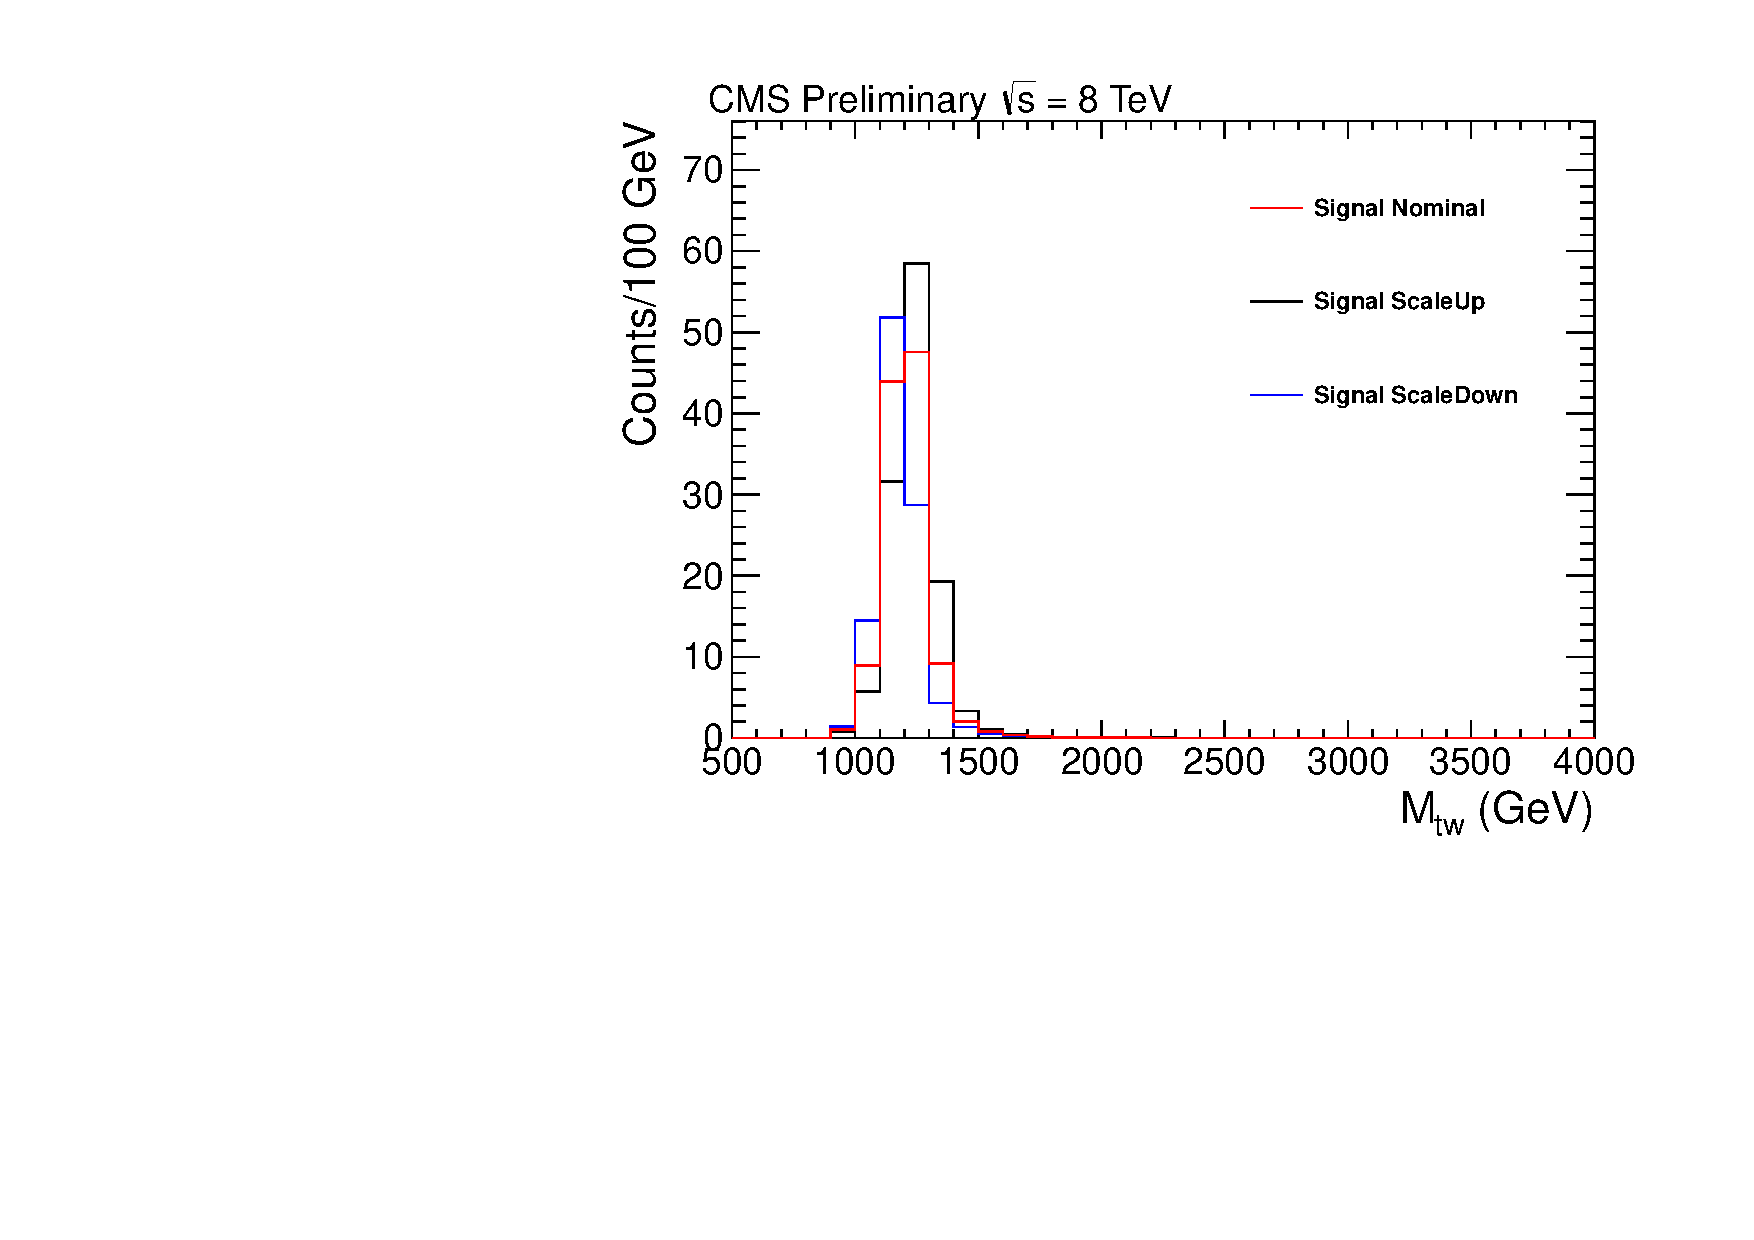
\includegraphics[width=0.4\textwidth]{AN-14-049/figs/Signal_M1200_PtScaling}
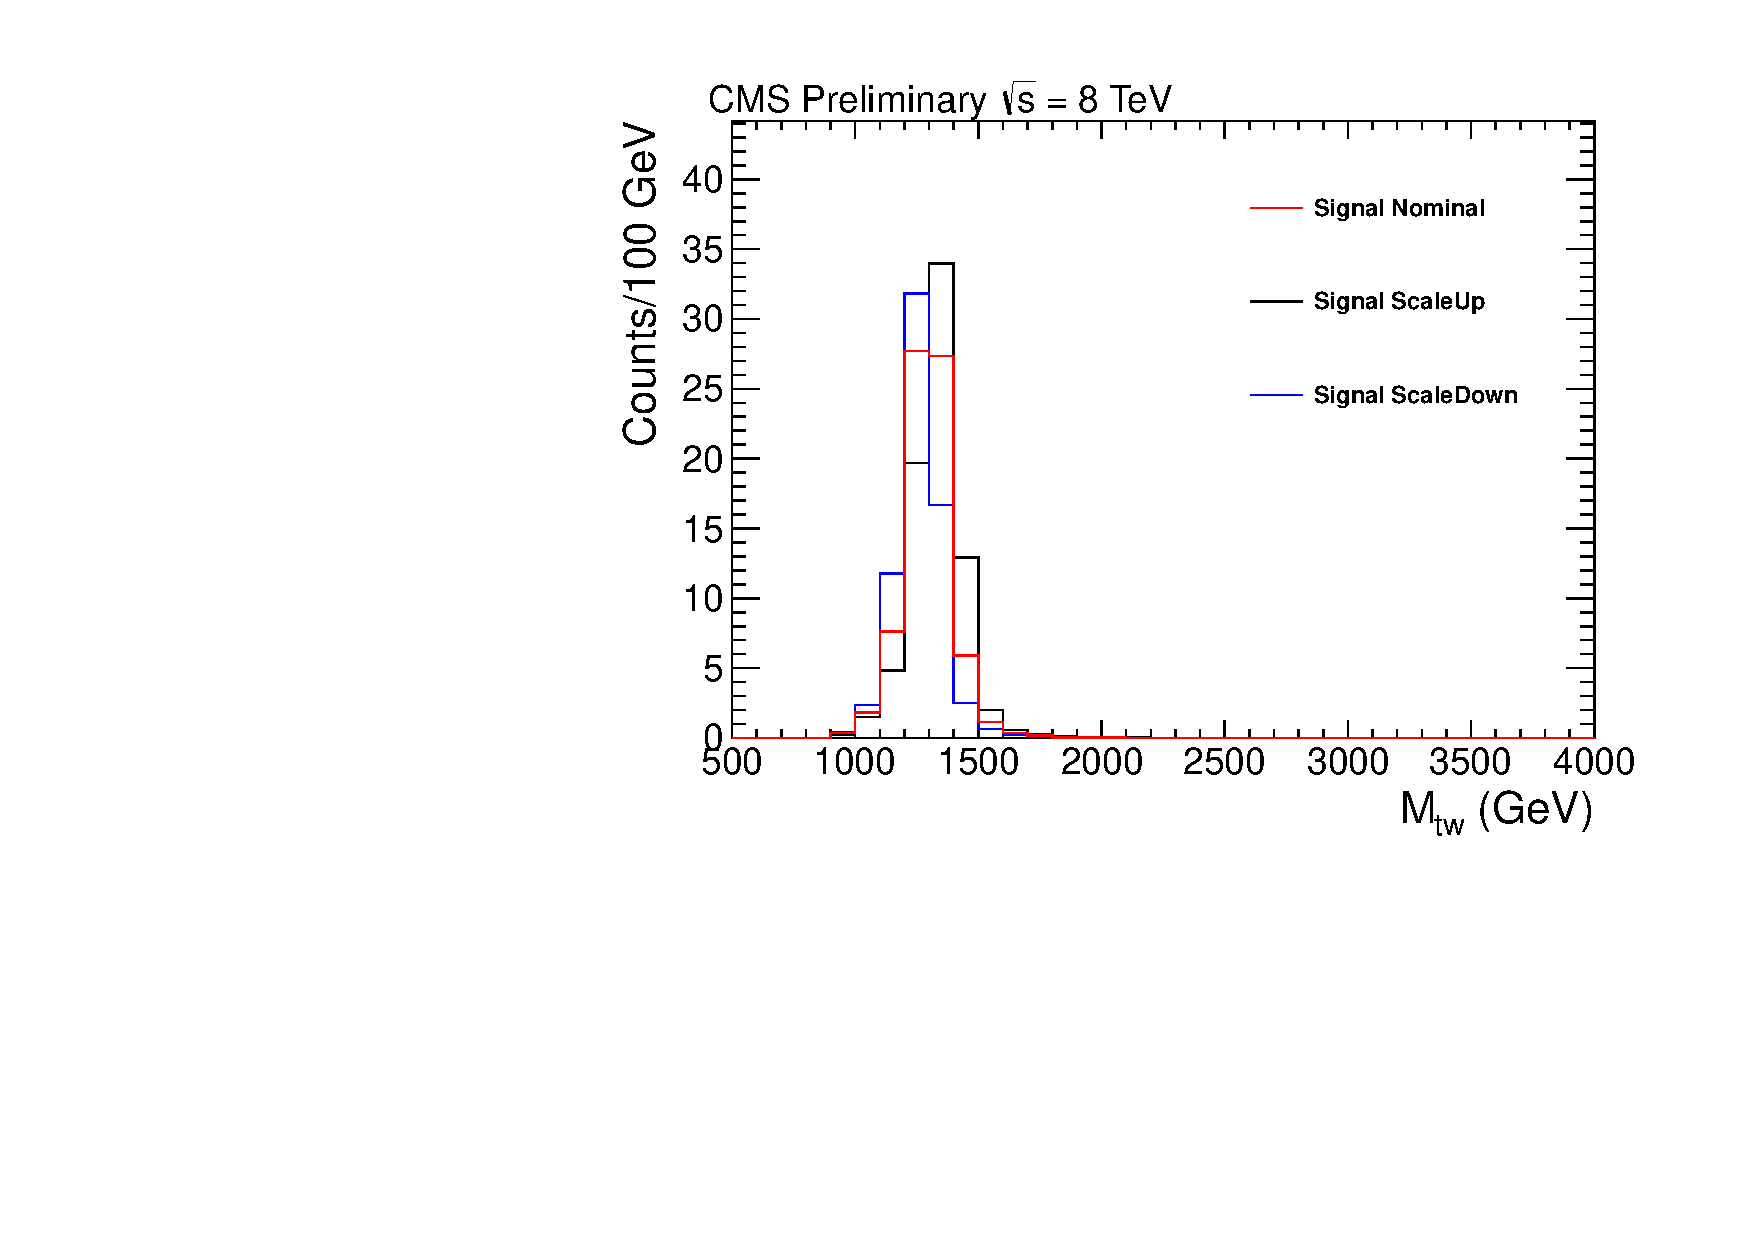
\includegraphics[width=0.4\textwidth]{AN-14-049/figs/Signal_M1300_PtScaling}
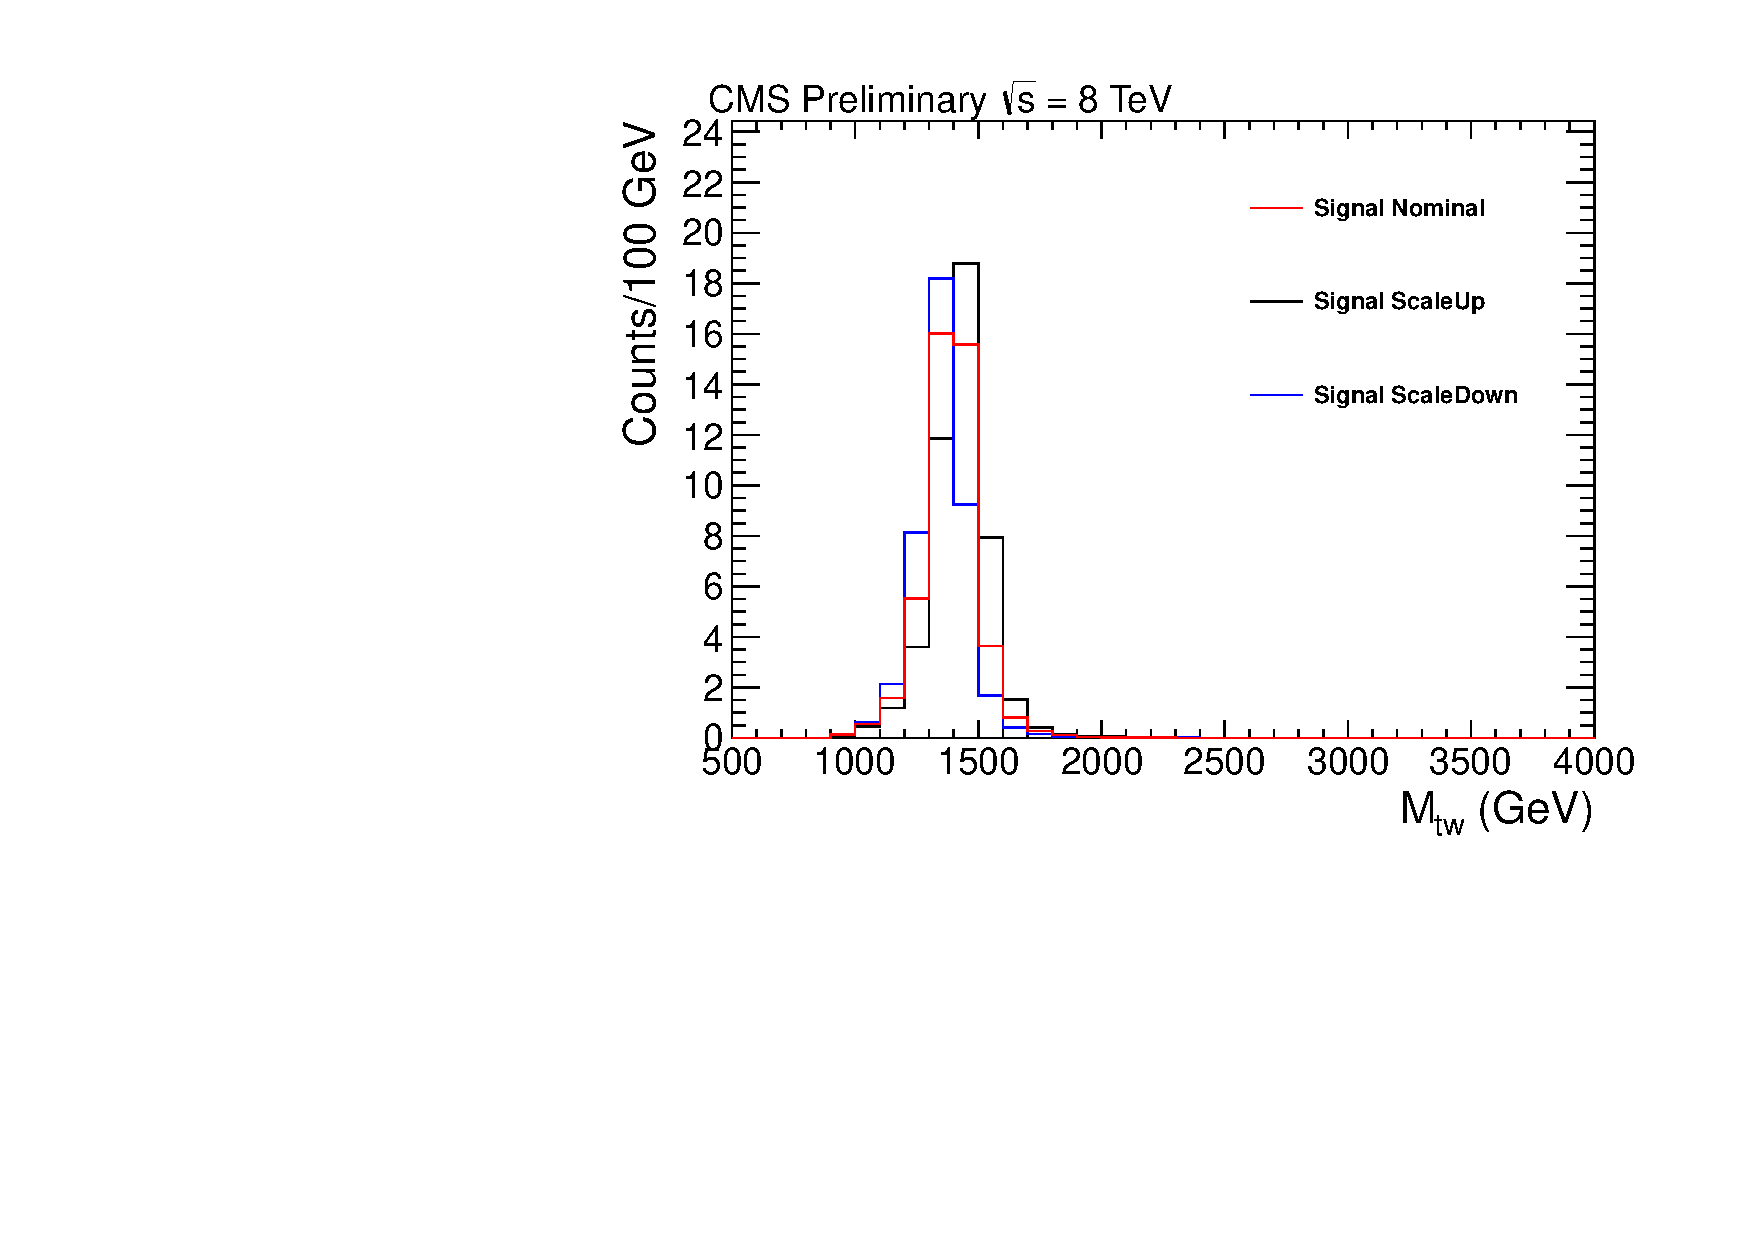
\includegraphics[width=0.4\textwidth]{AN-14-049/figs/Signal_M1400_PtScaling}
\caption{
Jet Energy Scale systematic variation for right-handed $\bs$  MC at the following mass points
(a) $\mathrm{M_{\bs}}$ = 1200$~\GeV$ 
(b) $\mathrm{M_{\bs}}$ = 1300$~\GeV$
(c) $\mathrm{M_{\bs}}$ = 1400$~\GeV$ 
}
\label{figs:bssignalJES}
\end{center}
\end{figure}

\begin{figure}[htcb]
\begin{center}
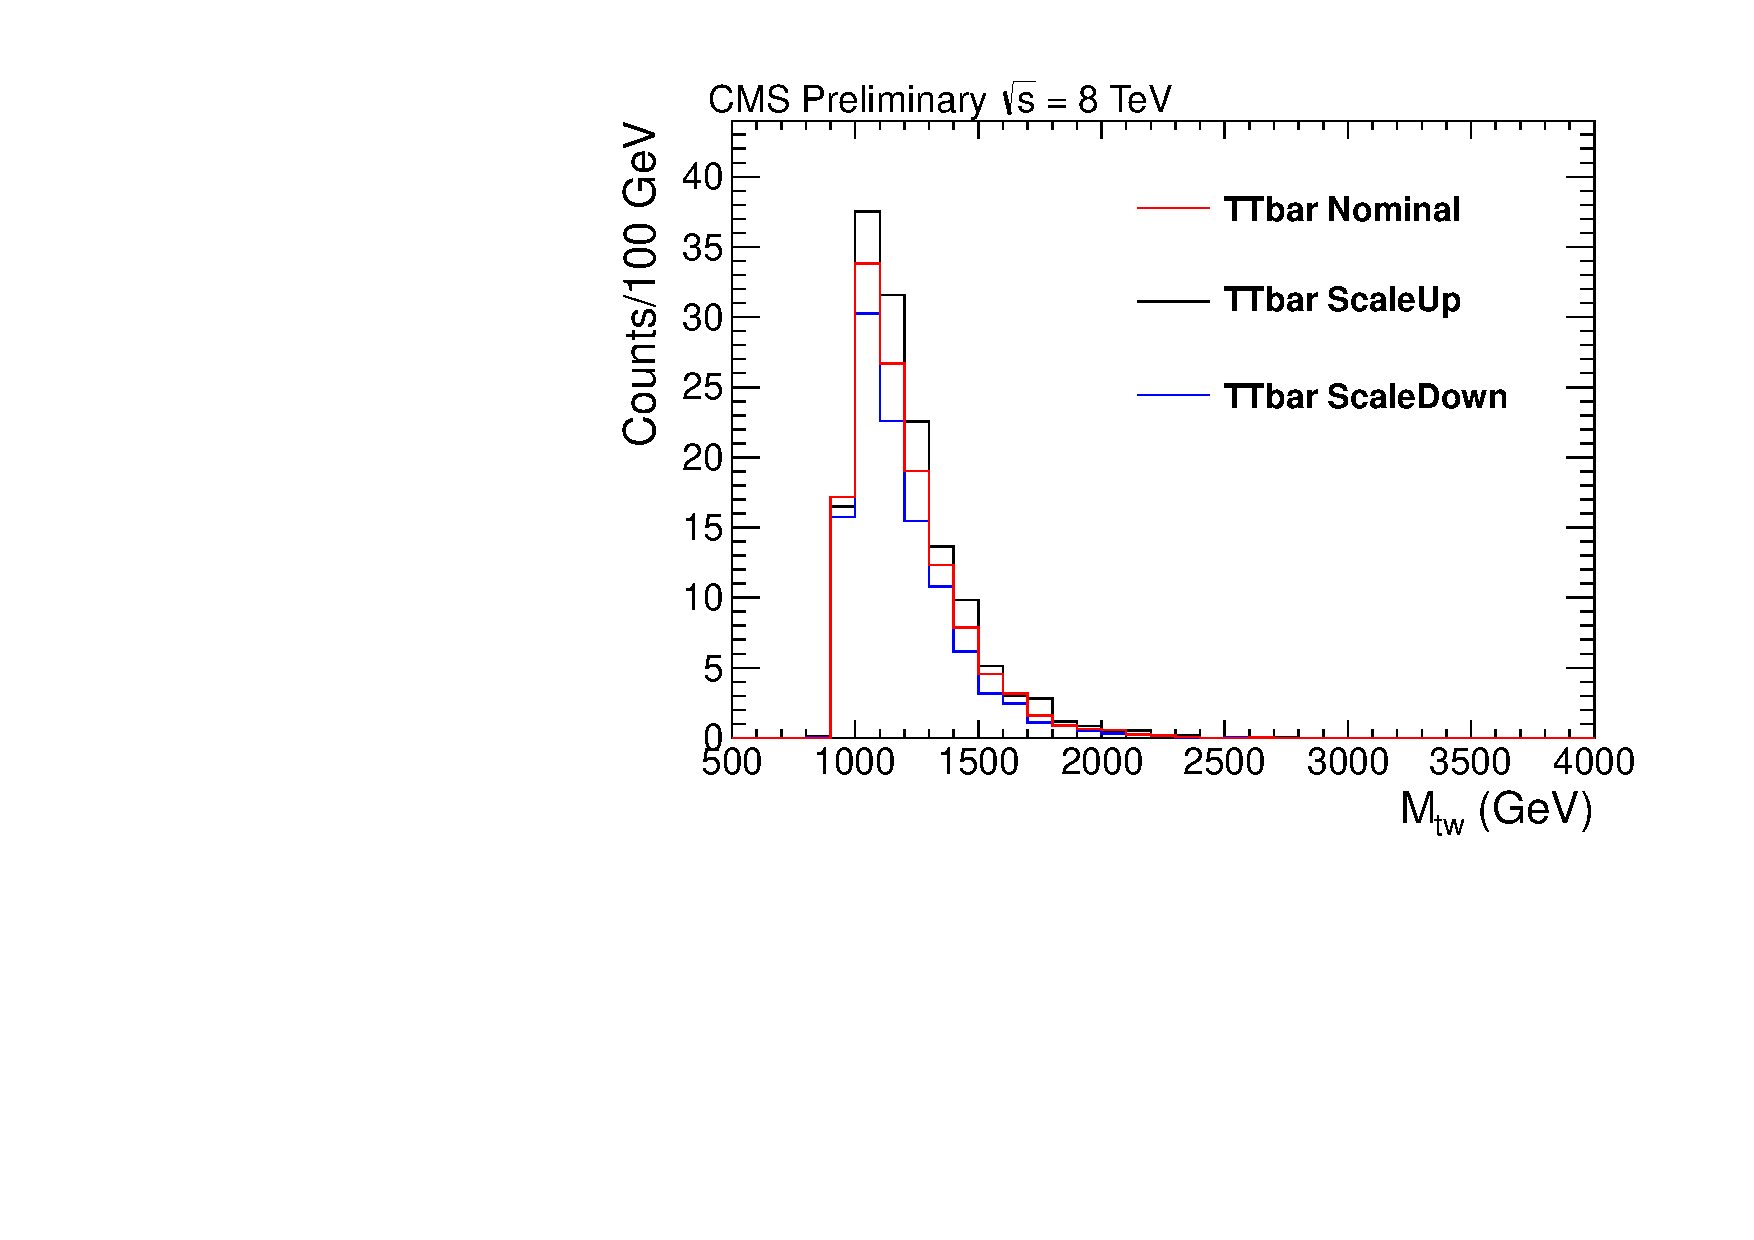
\includegraphics[width=0.7\textwidth]{AN-14-049/figs/TTbar_PtScaling}
\caption{Jet Energy Scale systematic variation for $\ttbar$ MC}
\label{figs:bsttbarJES}
\end{center}
\end{figure}

\begin{figure}[htcb]
\begin{center}
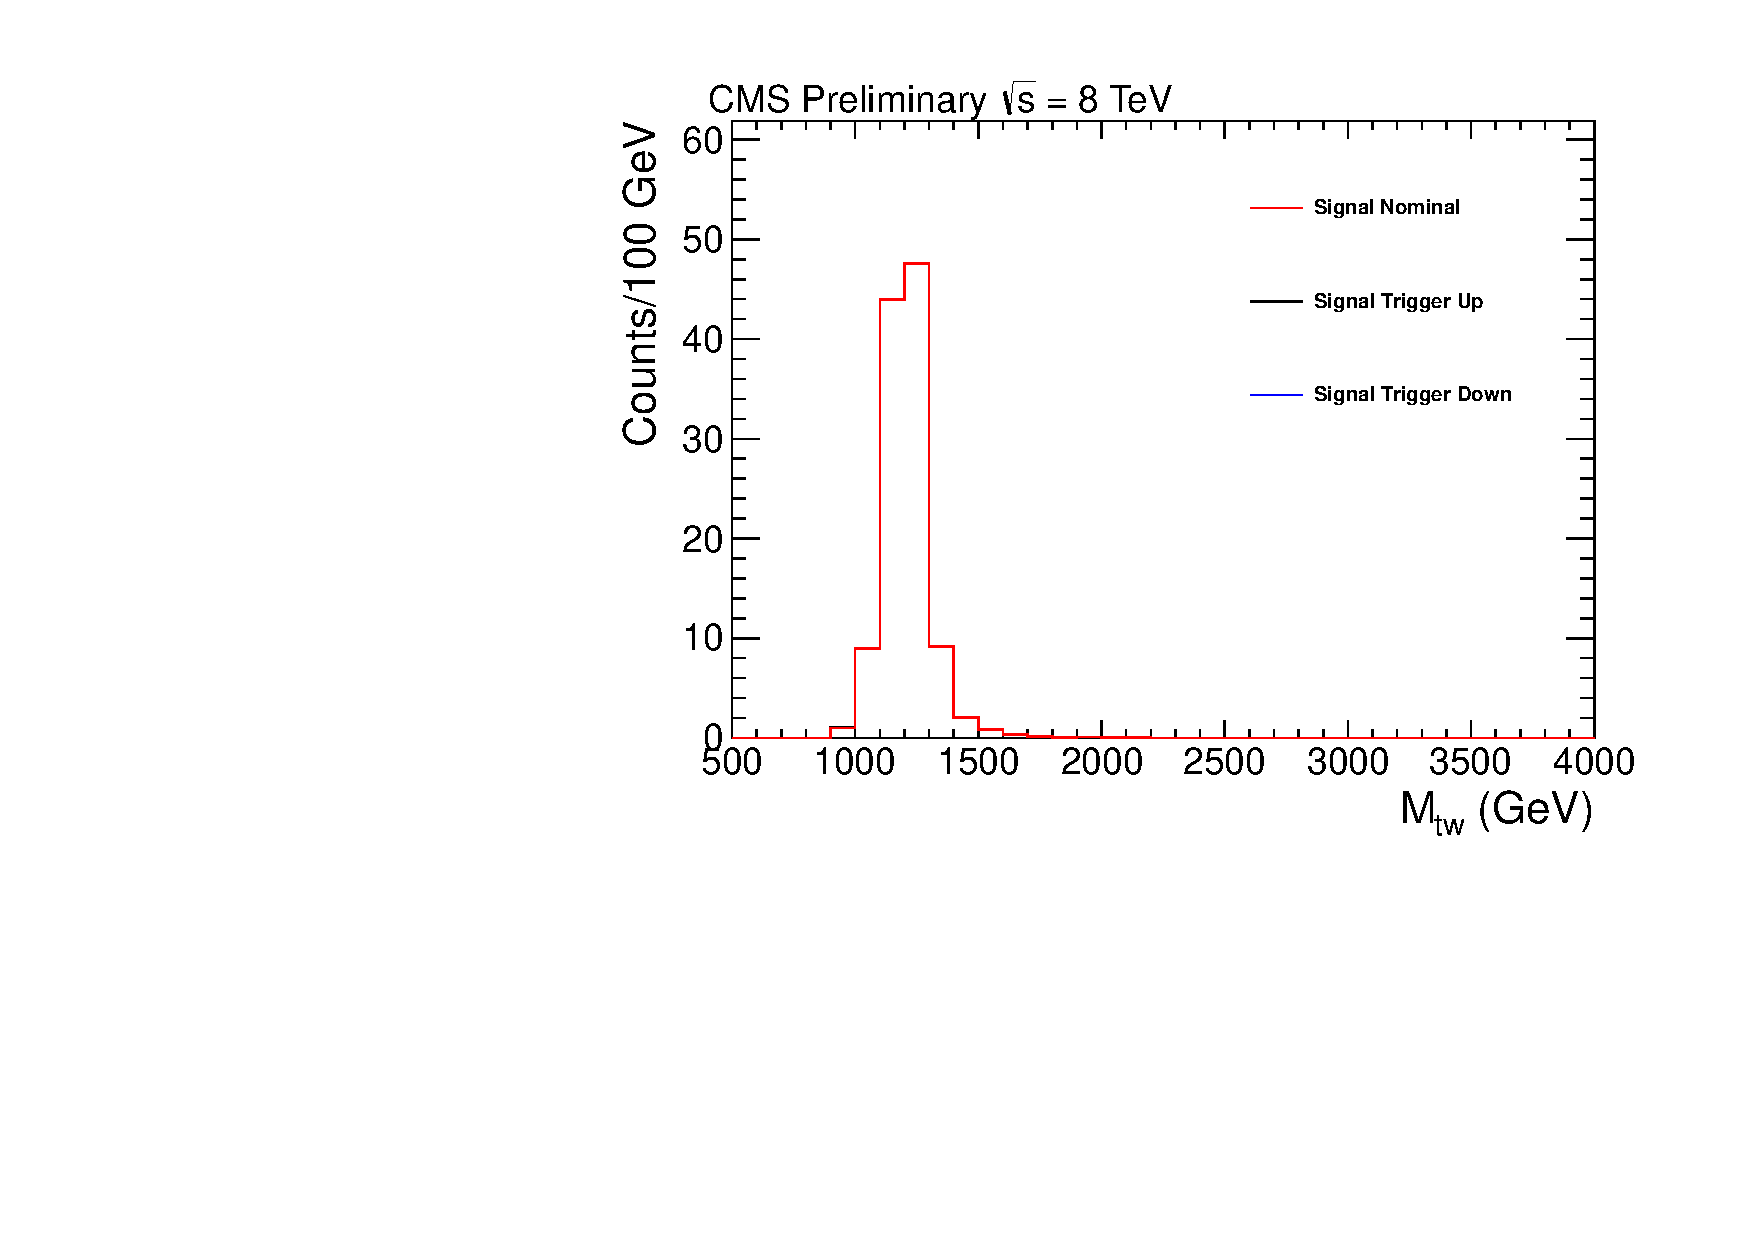
\includegraphics[width=0.45\textwidth]{AN-14-049/figs/Signal_M1200_TriggerWeighting}
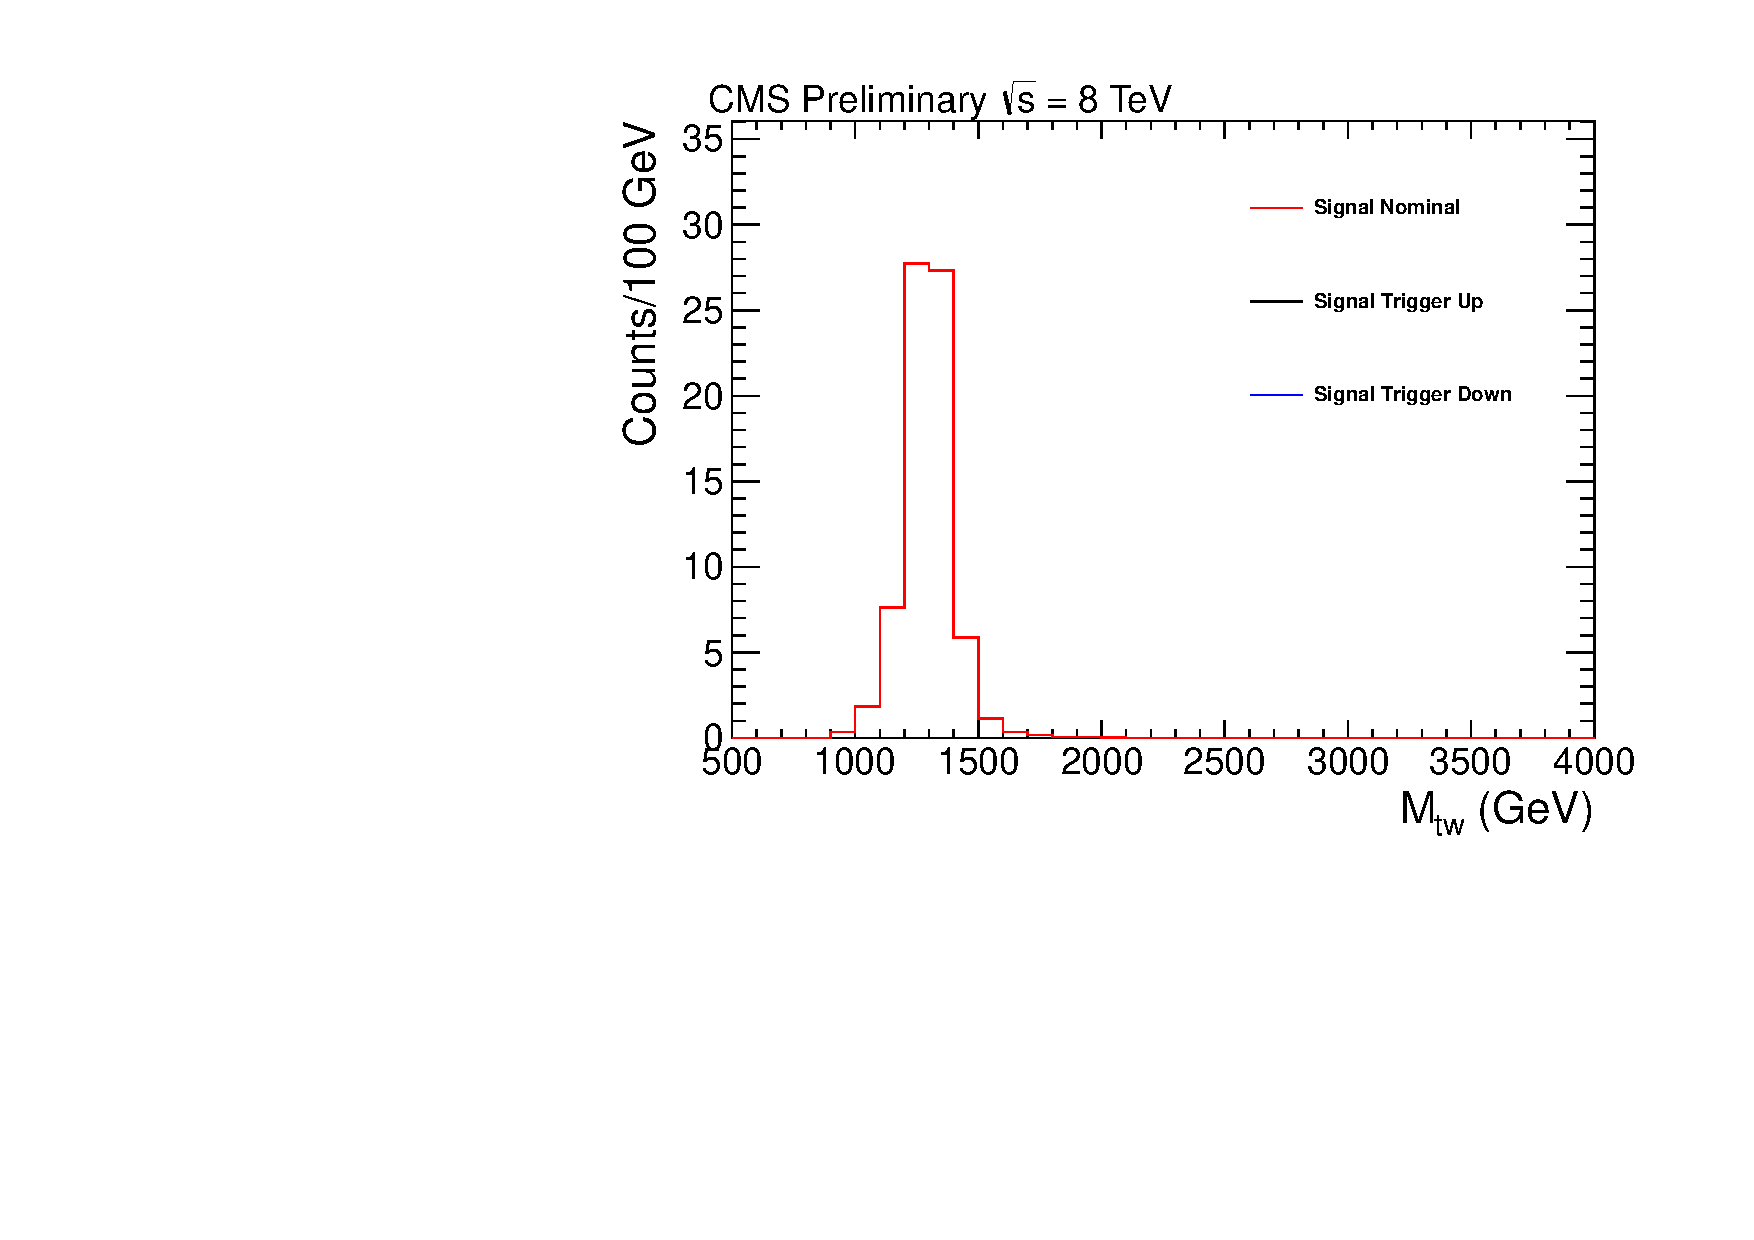
\includegraphics[width=0.45\textwidth]{AN-14-049/figs/Signal_M1300_TriggerWeighting}
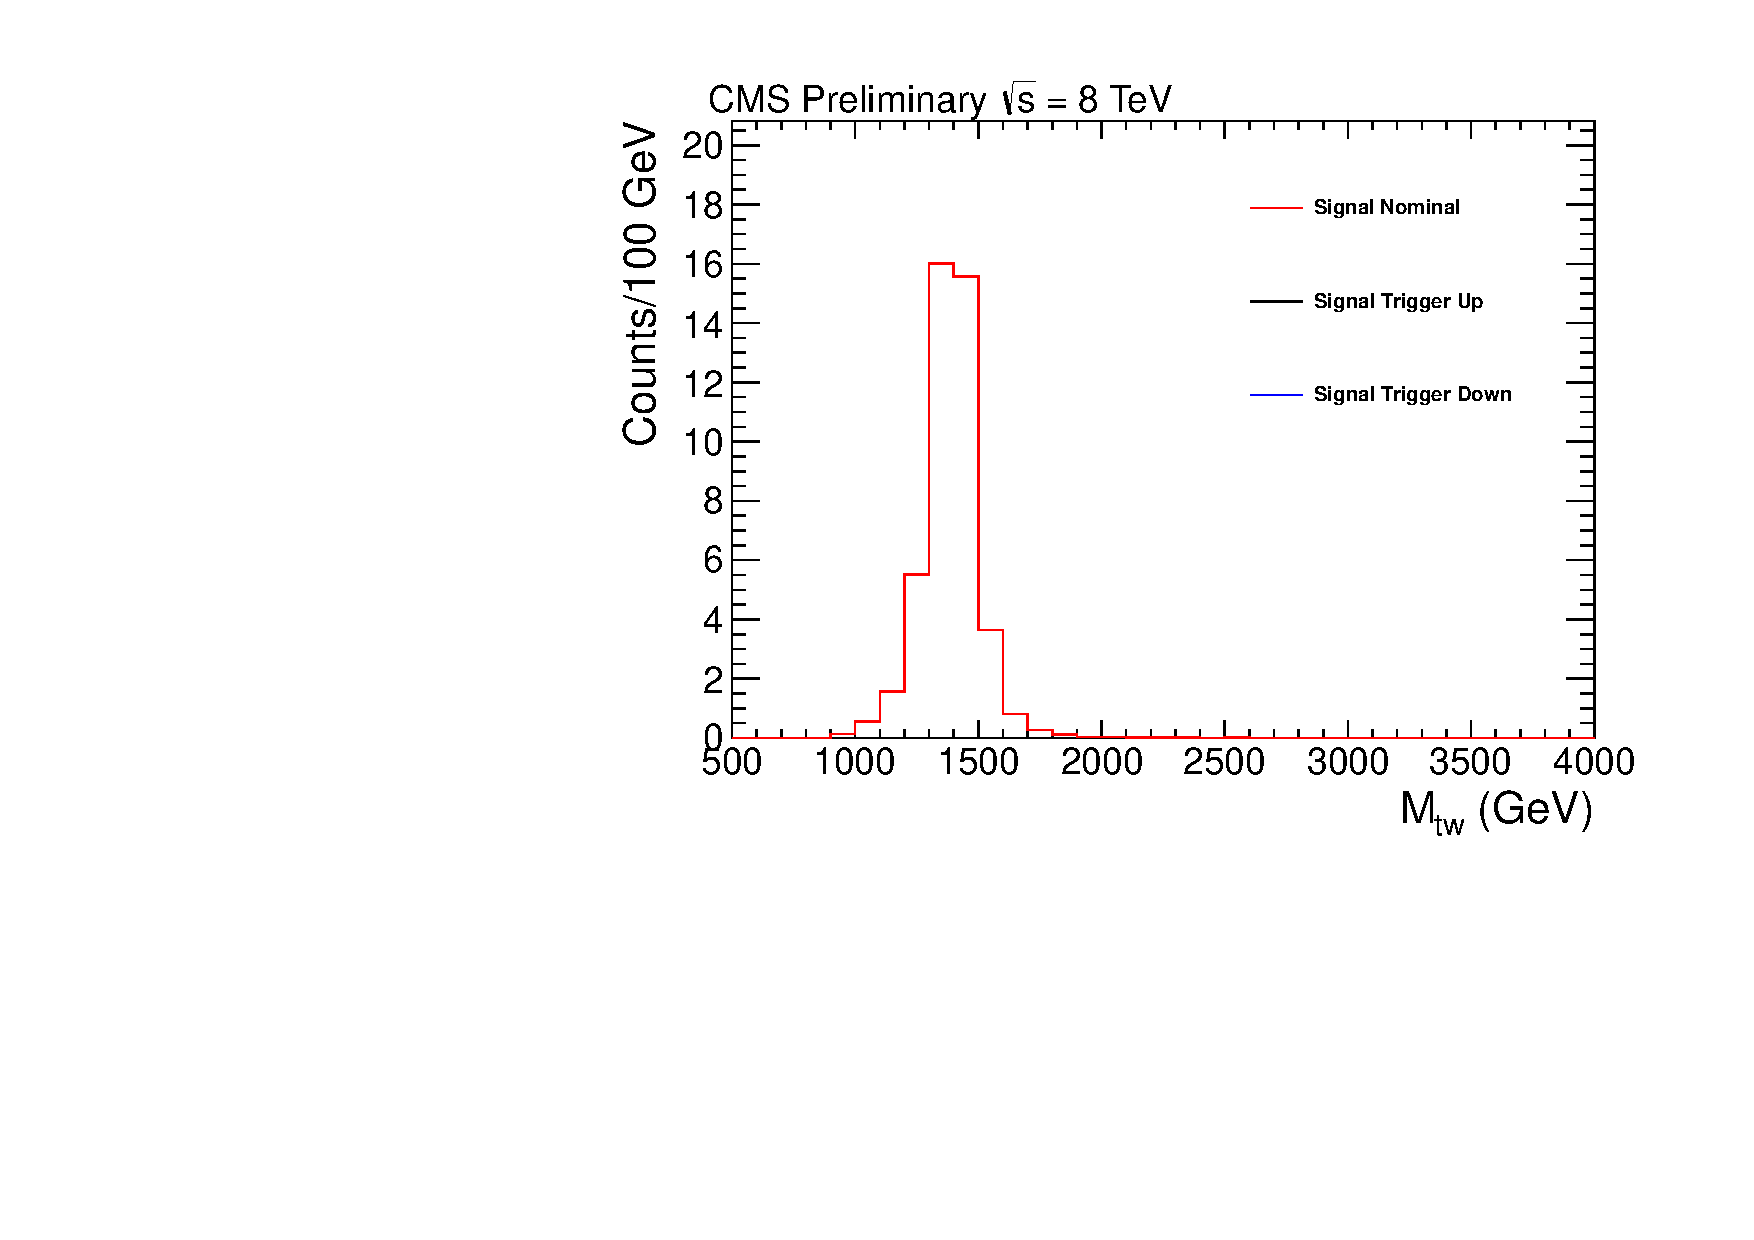
\includegraphics[width=0.45\textwidth]{AN-14-049/figs/Signal_M1400_TriggerWeighting}
\caption{
Trigger Weighting systematic variation for right-handed $\bs$  MC at the following mass points
(a) $\mathrm{M_{\bs}}$ = 1200$~\GeV$ 
(b) $\mathrm{M_{\bs}}$ = 1300$~\GeV$
(c) $\mathrm{M_{\bs}}$ = 1400$~\GeV$ 
}
\label{figs:bssignaltrig}
\end{center}
\end{figure}

\begin{figure}[htcb]
\begin{center}
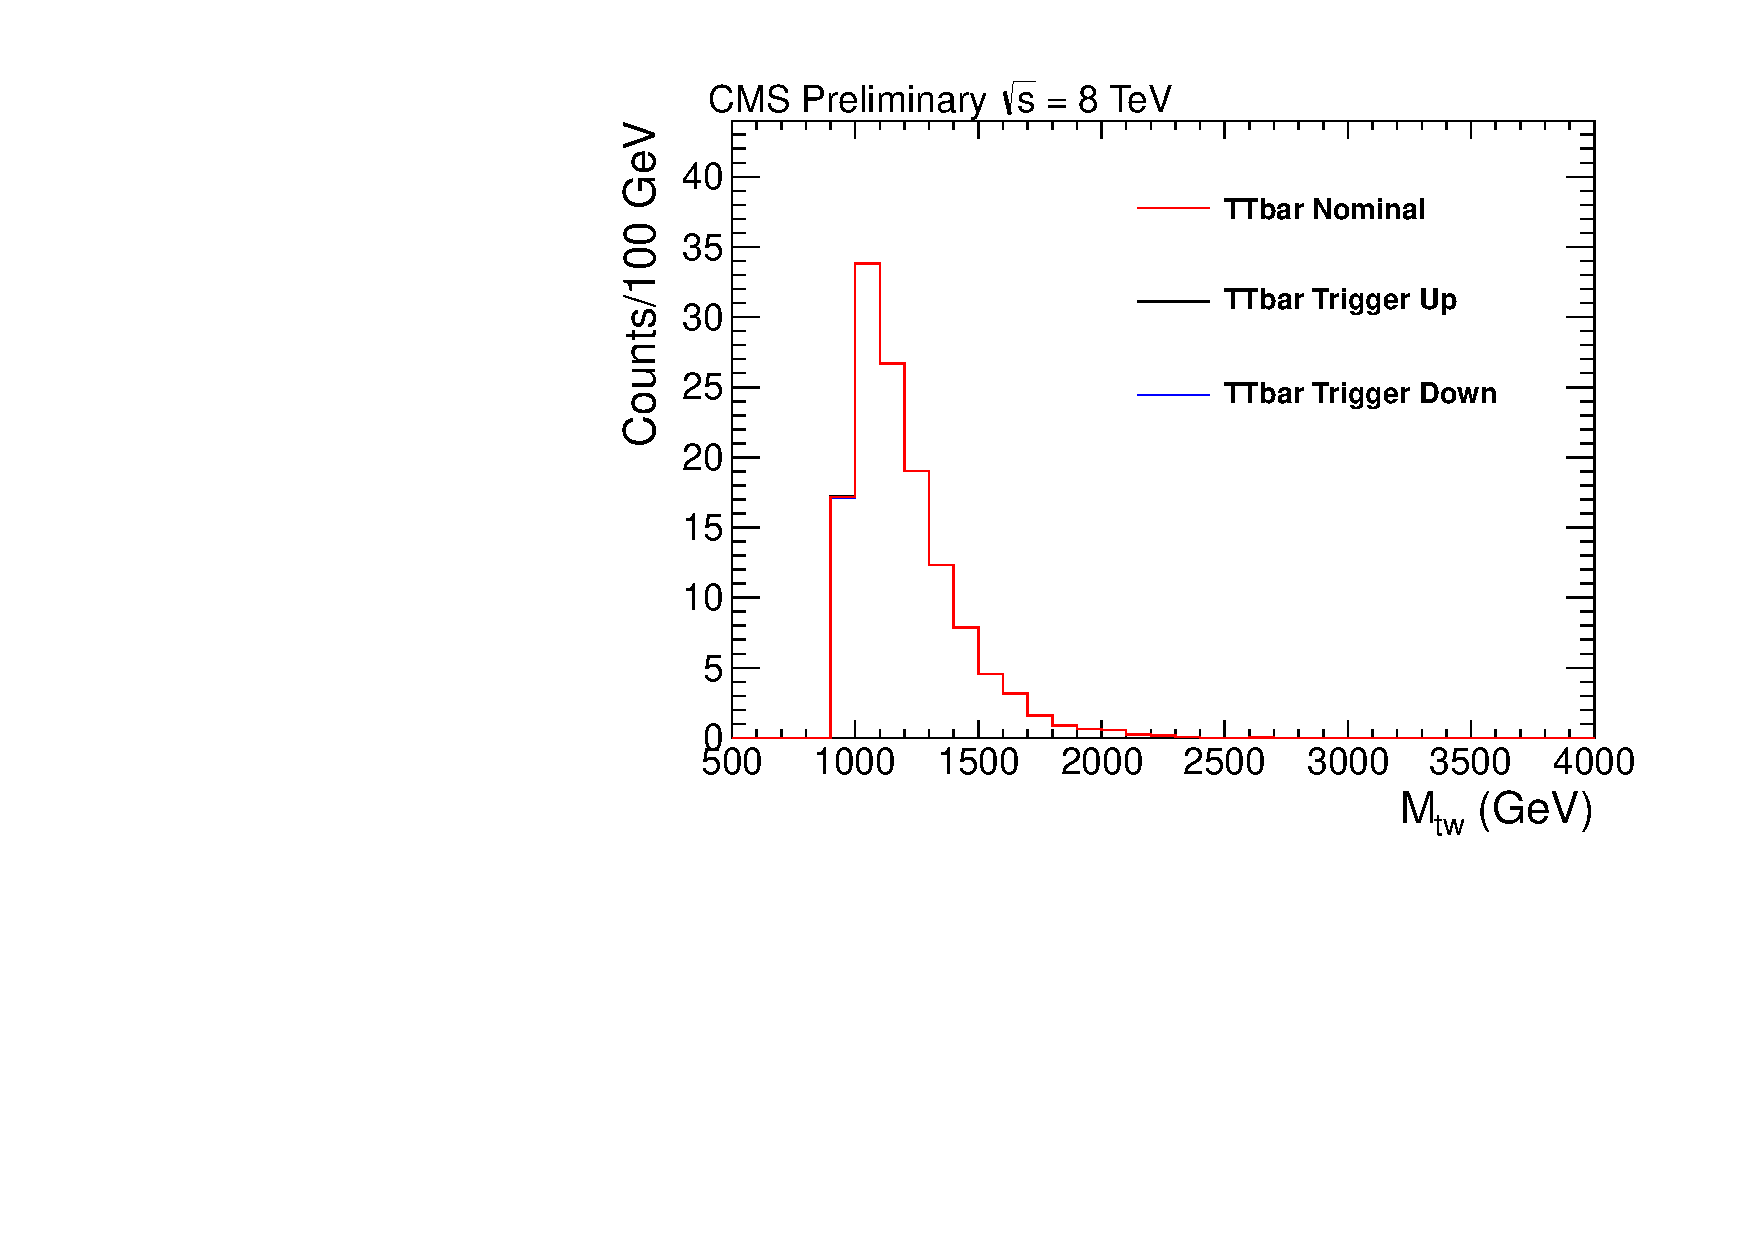
\includegraphics[width=0.7\textwidth]{AN-14-049/figs/TTbar_TriggerWeighting}
\caption{Trigger Weighting systematic variation for $\ttbar$ MC}
\label{figs:bsttbartrig}
\end{center}
\end{figure}


\begin{figure}[htcb]
\begin{center}
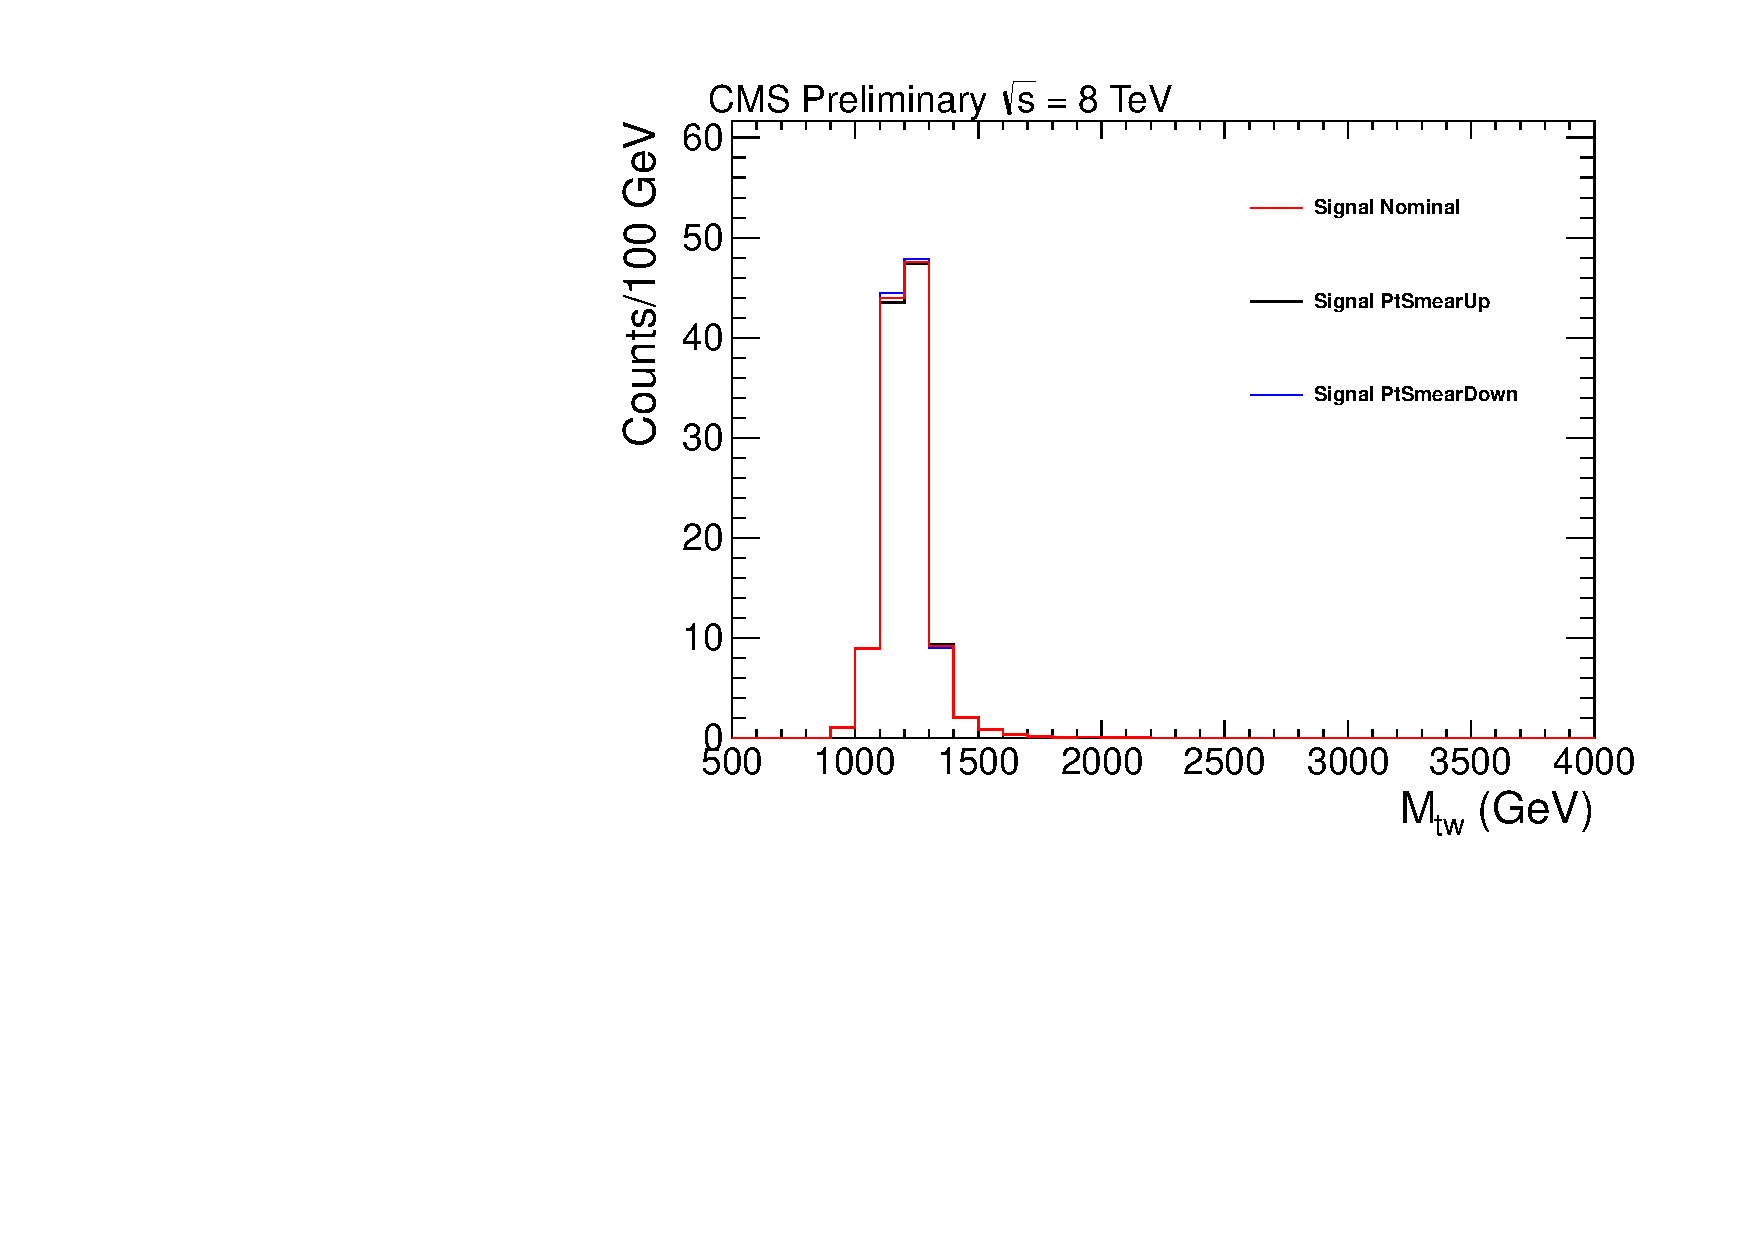
\includegraphics[width=0.45\textwidth]{AN-14-049/figs/Signal_M1200_PtSmearing}
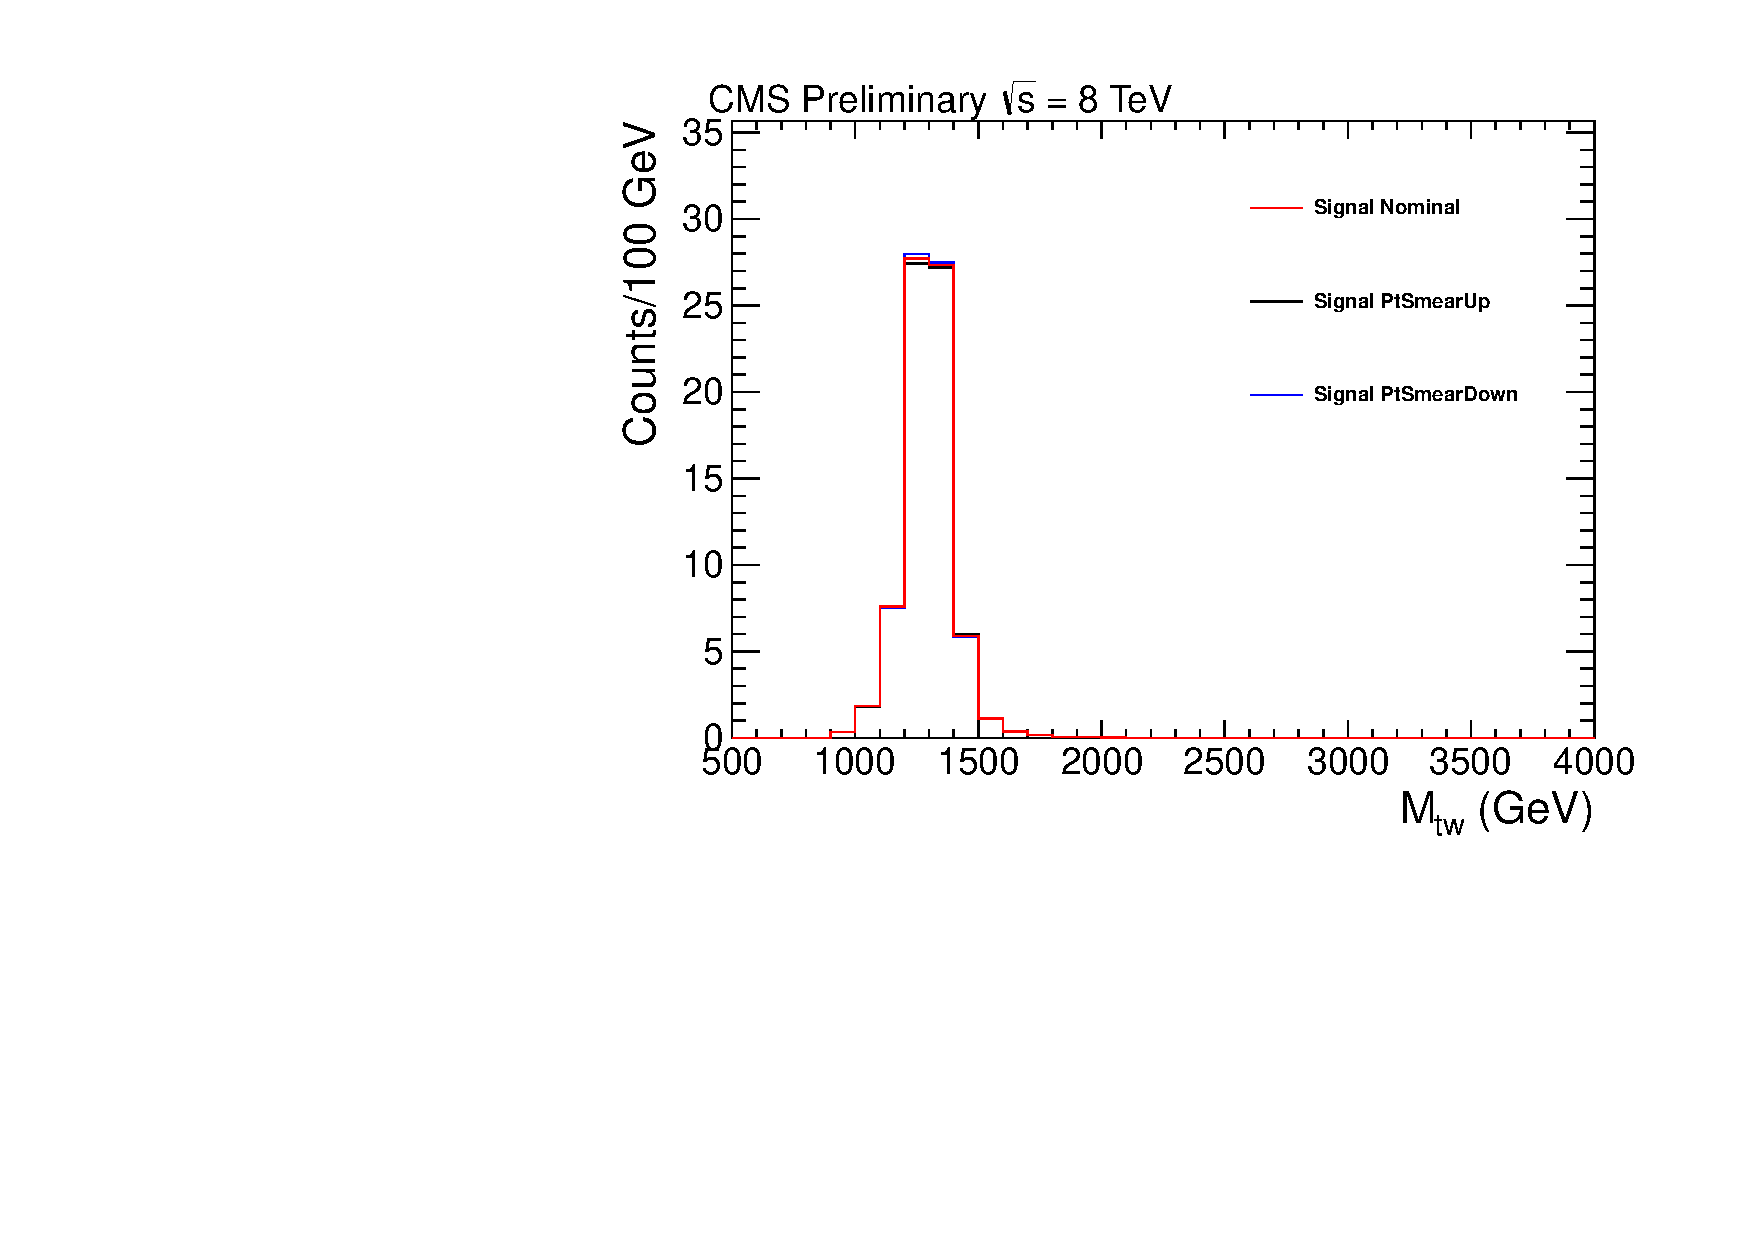
\includegraphics[width=0.45\textwidth]{AN-14-049/figs/Signal_M1300_PtSmearing}
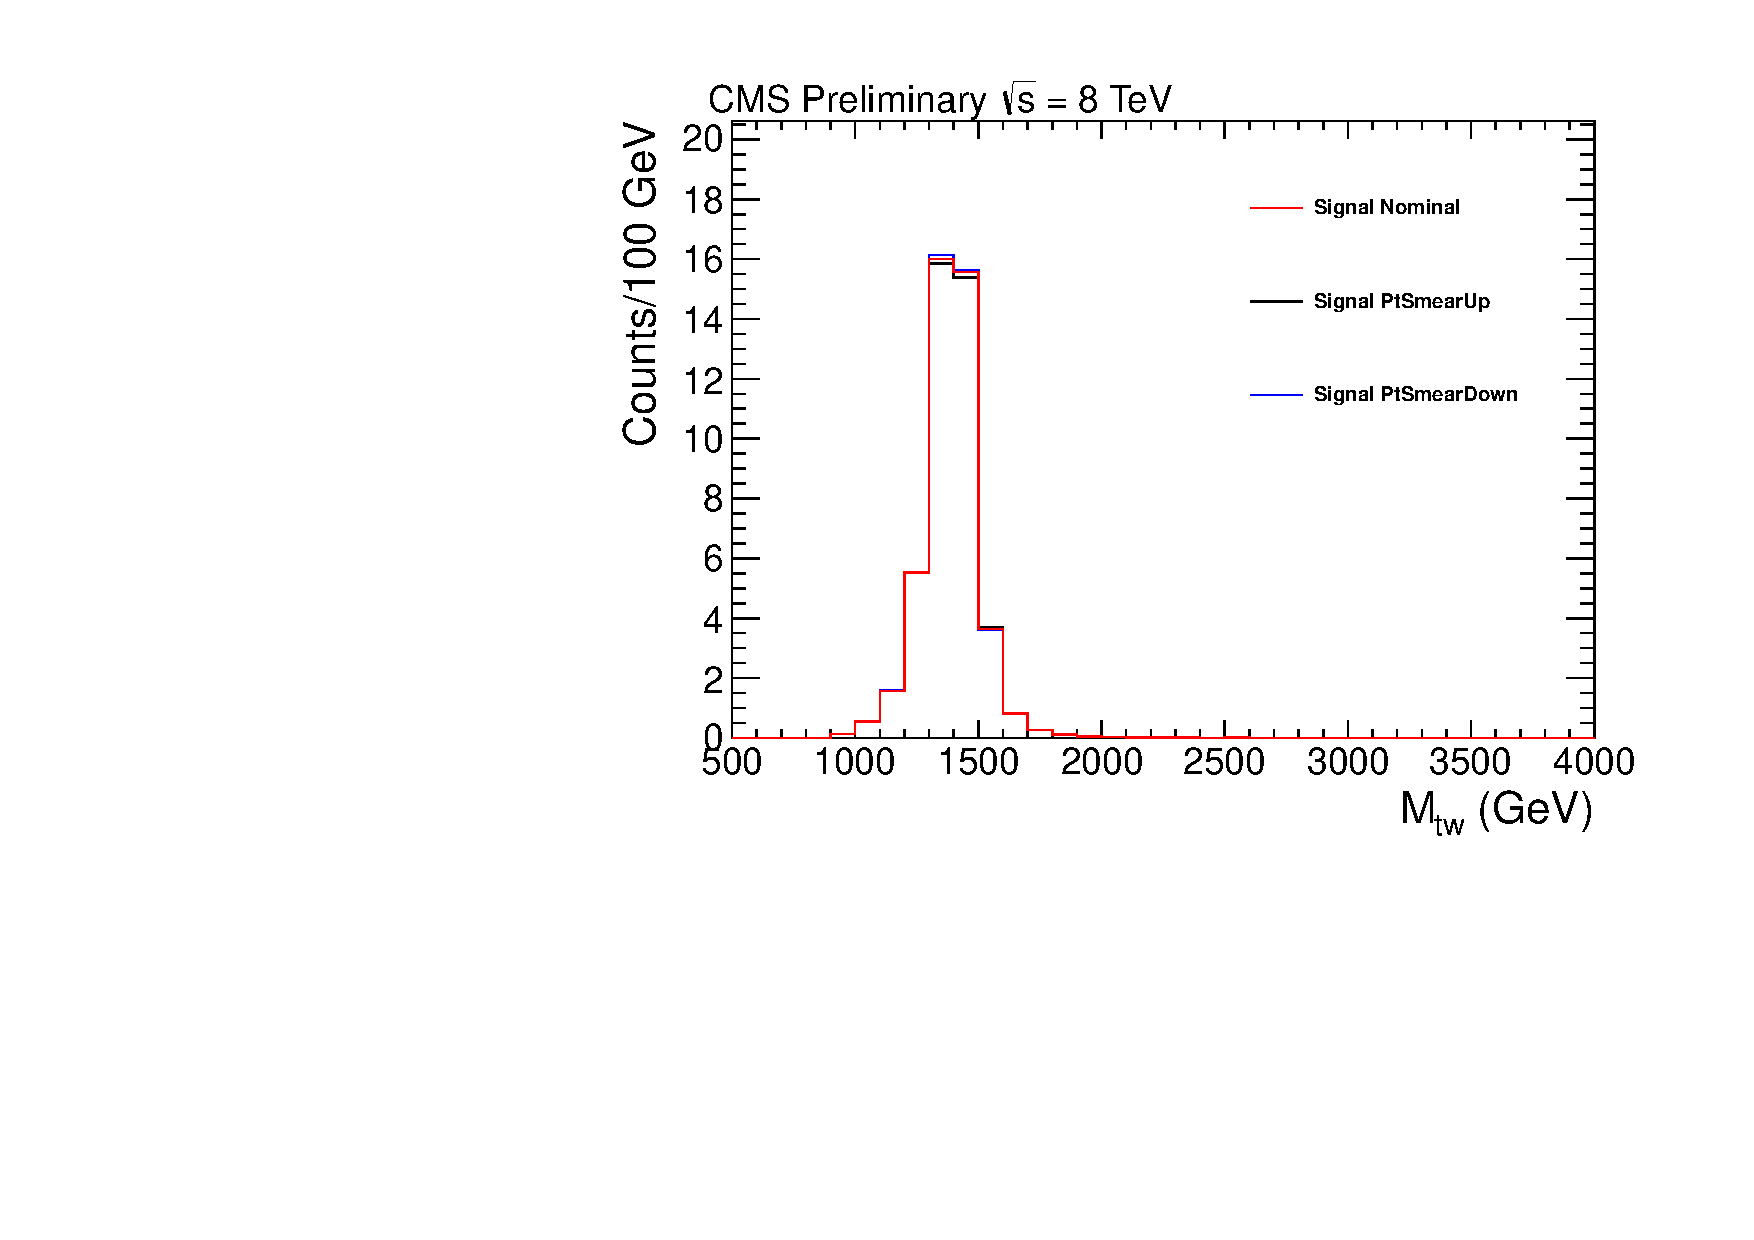
\includegraphics[width=0.45\textwidth]{AN-14-049/figs/Signal_M1400_PtSmearing}
\caption{
Jet Energy Resolution systematic variation for right-handed $\bs$  MC at the following mass points
(a) $\mathrm{M_{\bs}}$ = 1200$~\GeV$ 
(b) $\mathrm{M_{\bs}}$ = 1300$~\GeV$
(c) $\mathrm{M_{\bs}}$ = 1400$~\GeV$ 
}
\label{figs:bssignalJER}
\end{center}
\end{figure}

\begin{figure}[htcb]
\begin{center}
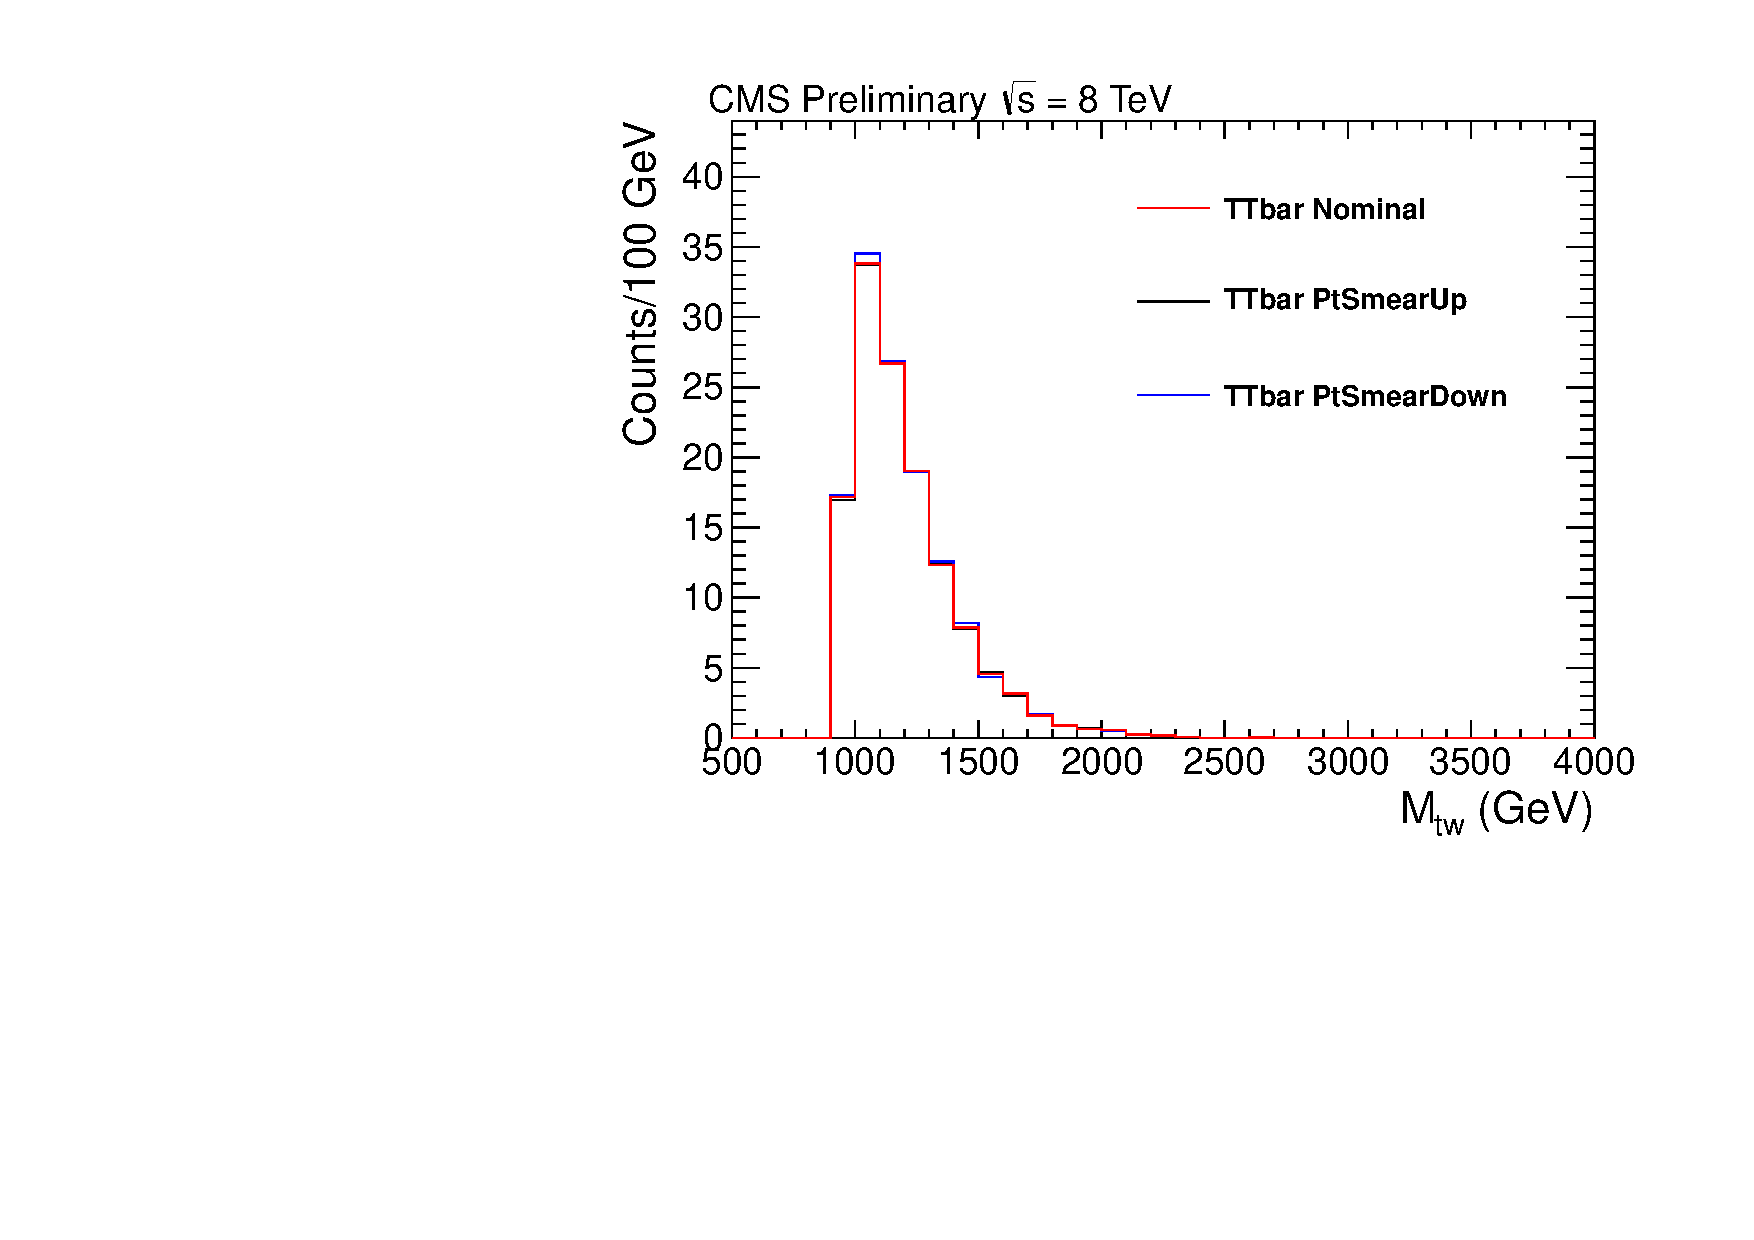
\includegraphics[width=0.7\textwidth]{AN-14-049/figs/TTbar_PtSmearing}
\caption{Jet Energy Resolution systematic variation for $\ttbar$ MC}
\label{figs:bsttbarJER}
\end{center}
\end{figure}

\begin{figure}[htcb]
\begin{center}
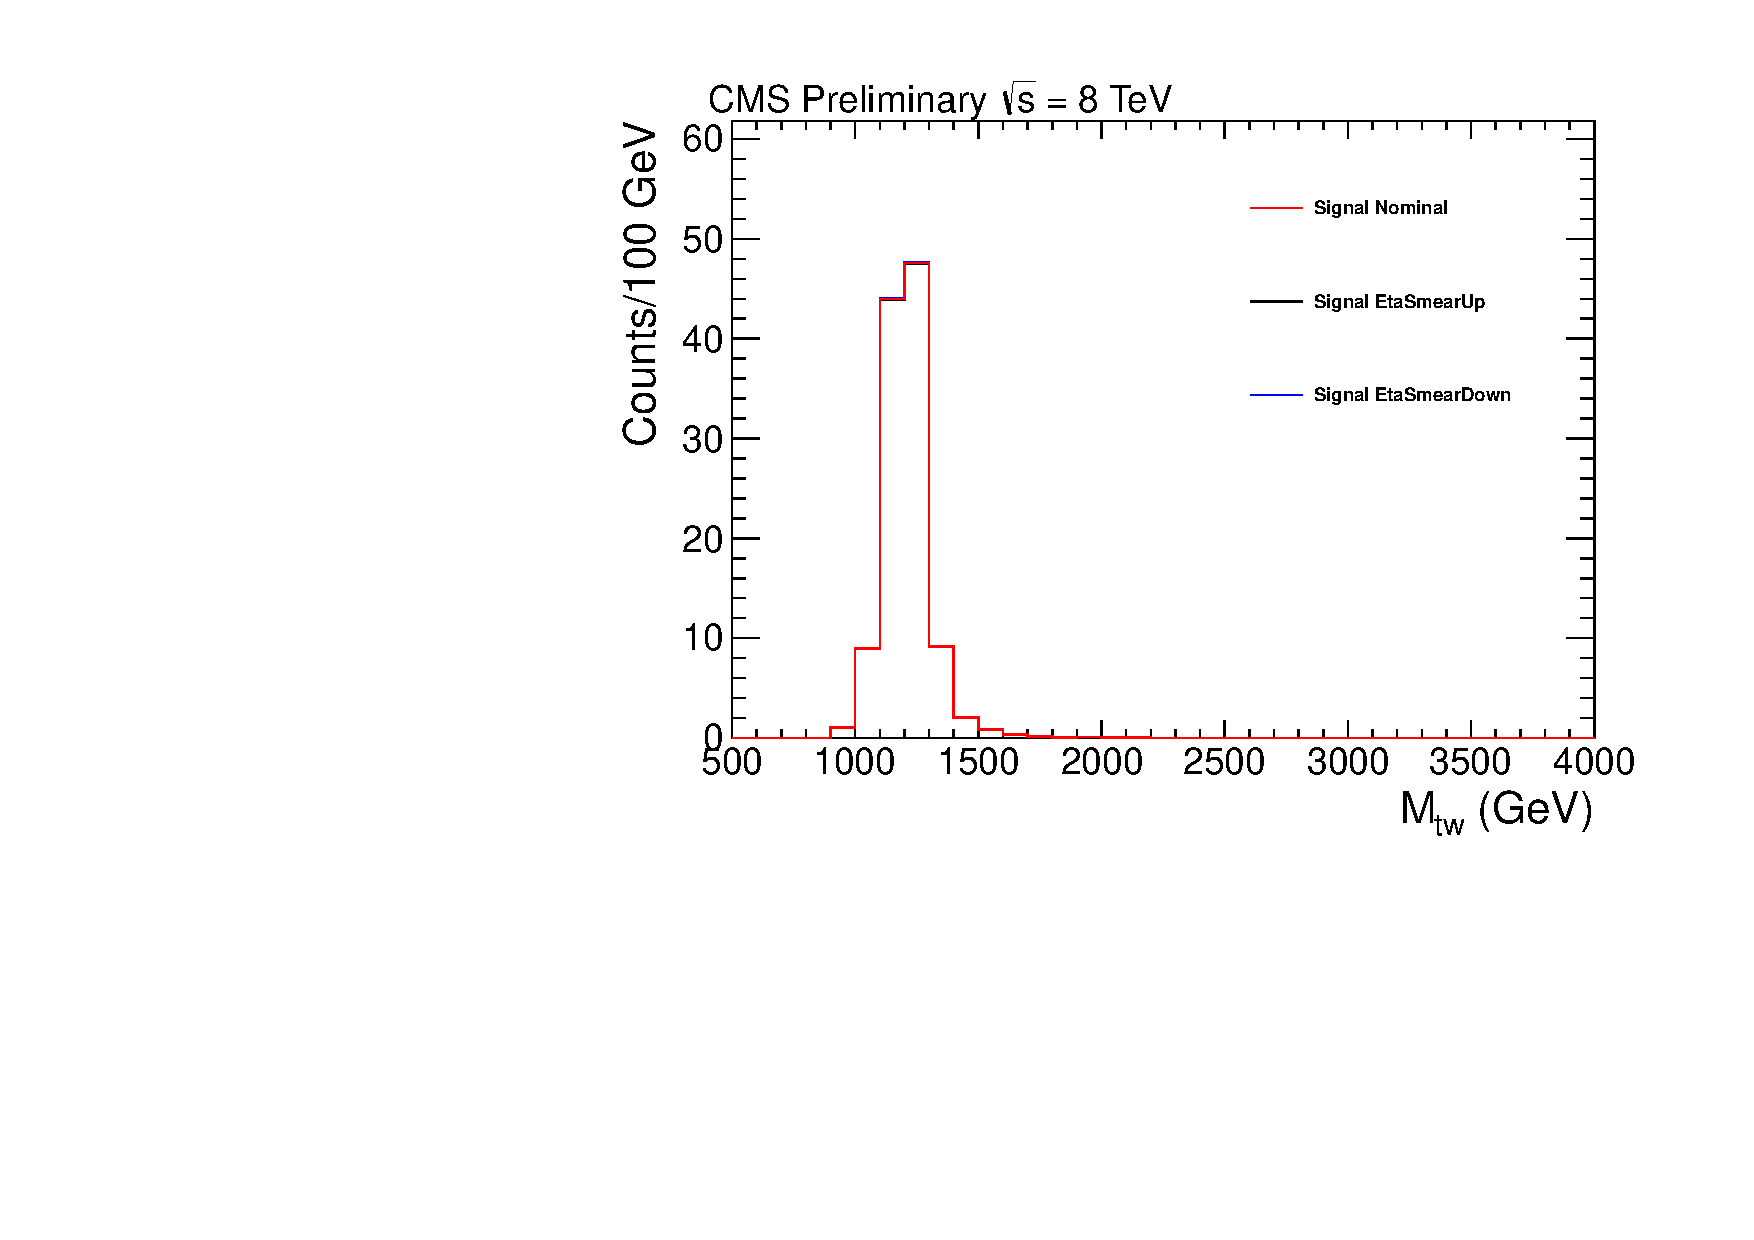
\includegraphics[width=0.45\textwidth]{AN-14-049/figs/Signal_M1200_EtaScaling}
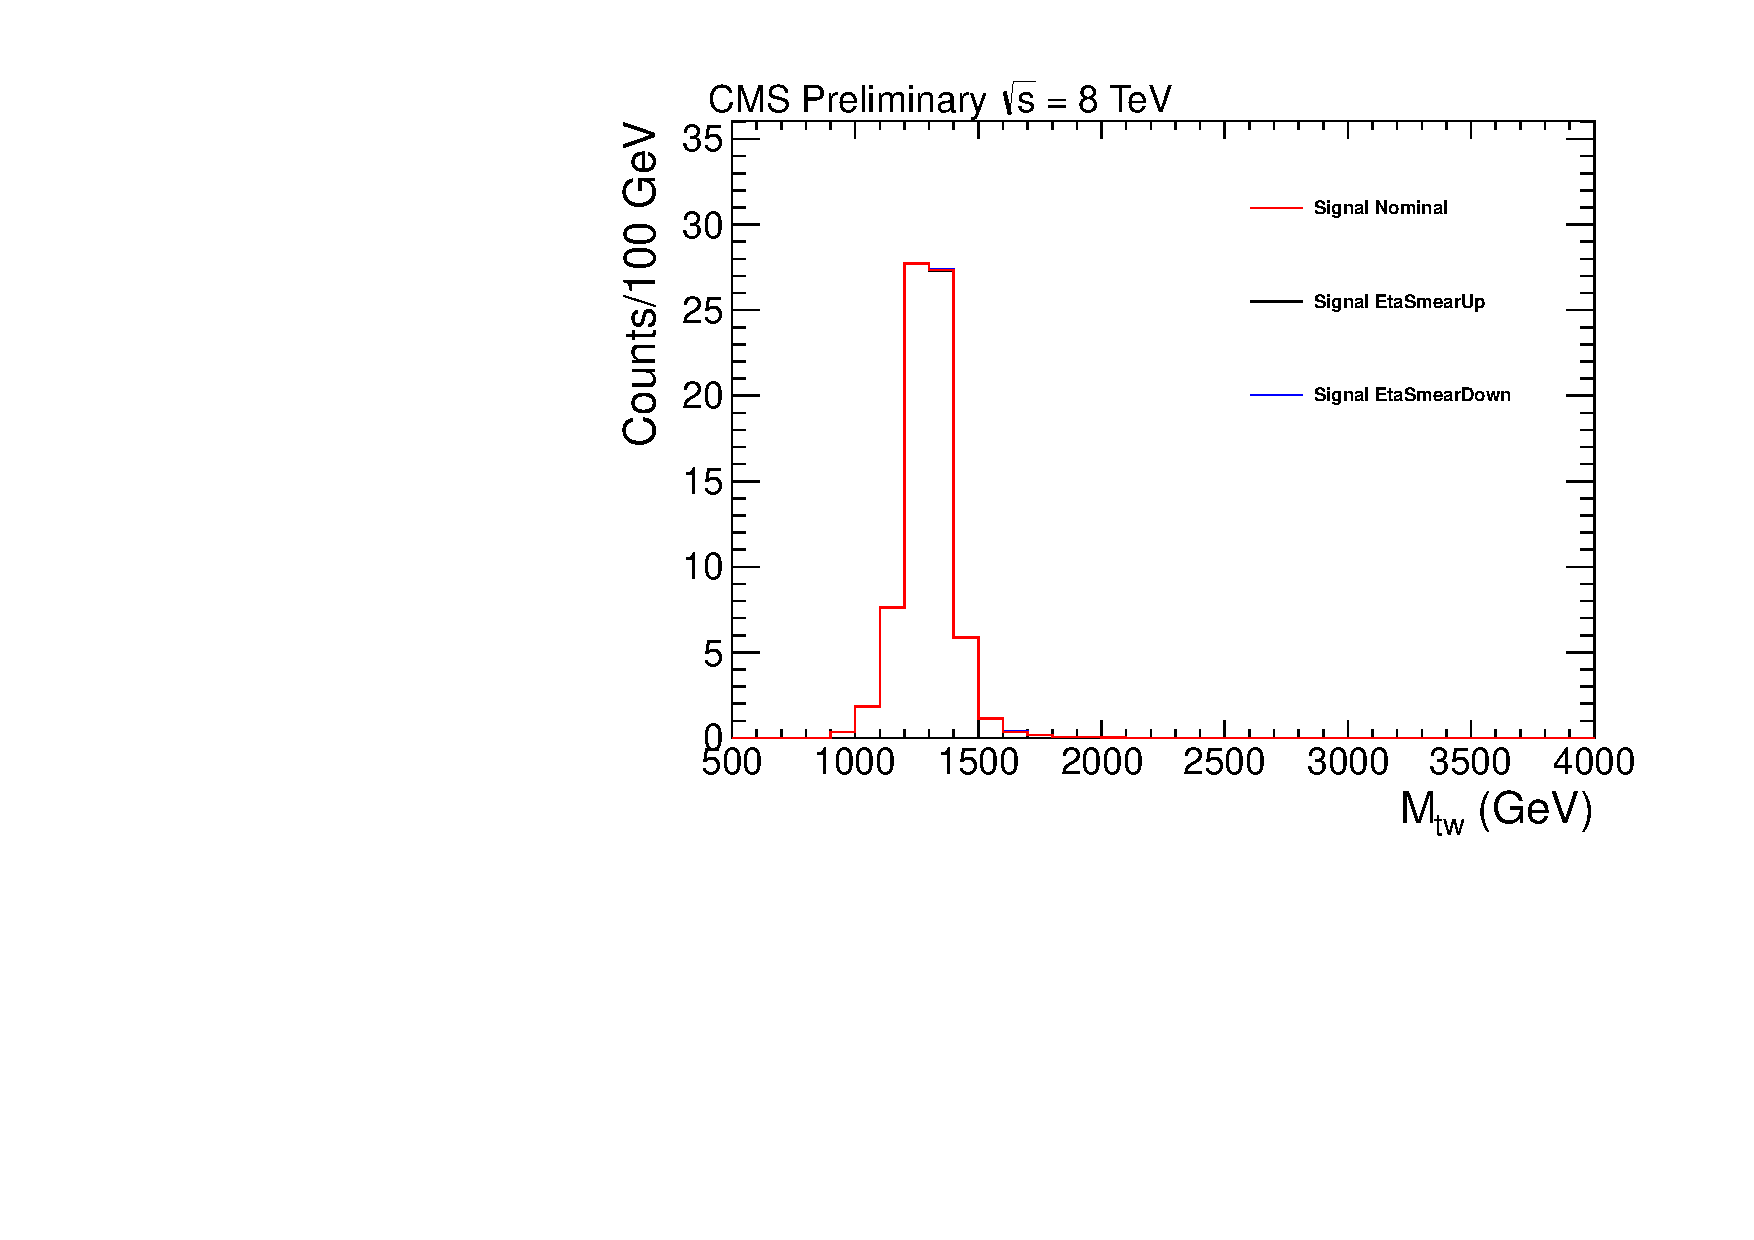
\includegraphics[width=0.45\textwidth]{AN-14-049/figs/Signal_M1300_EtaScaling}
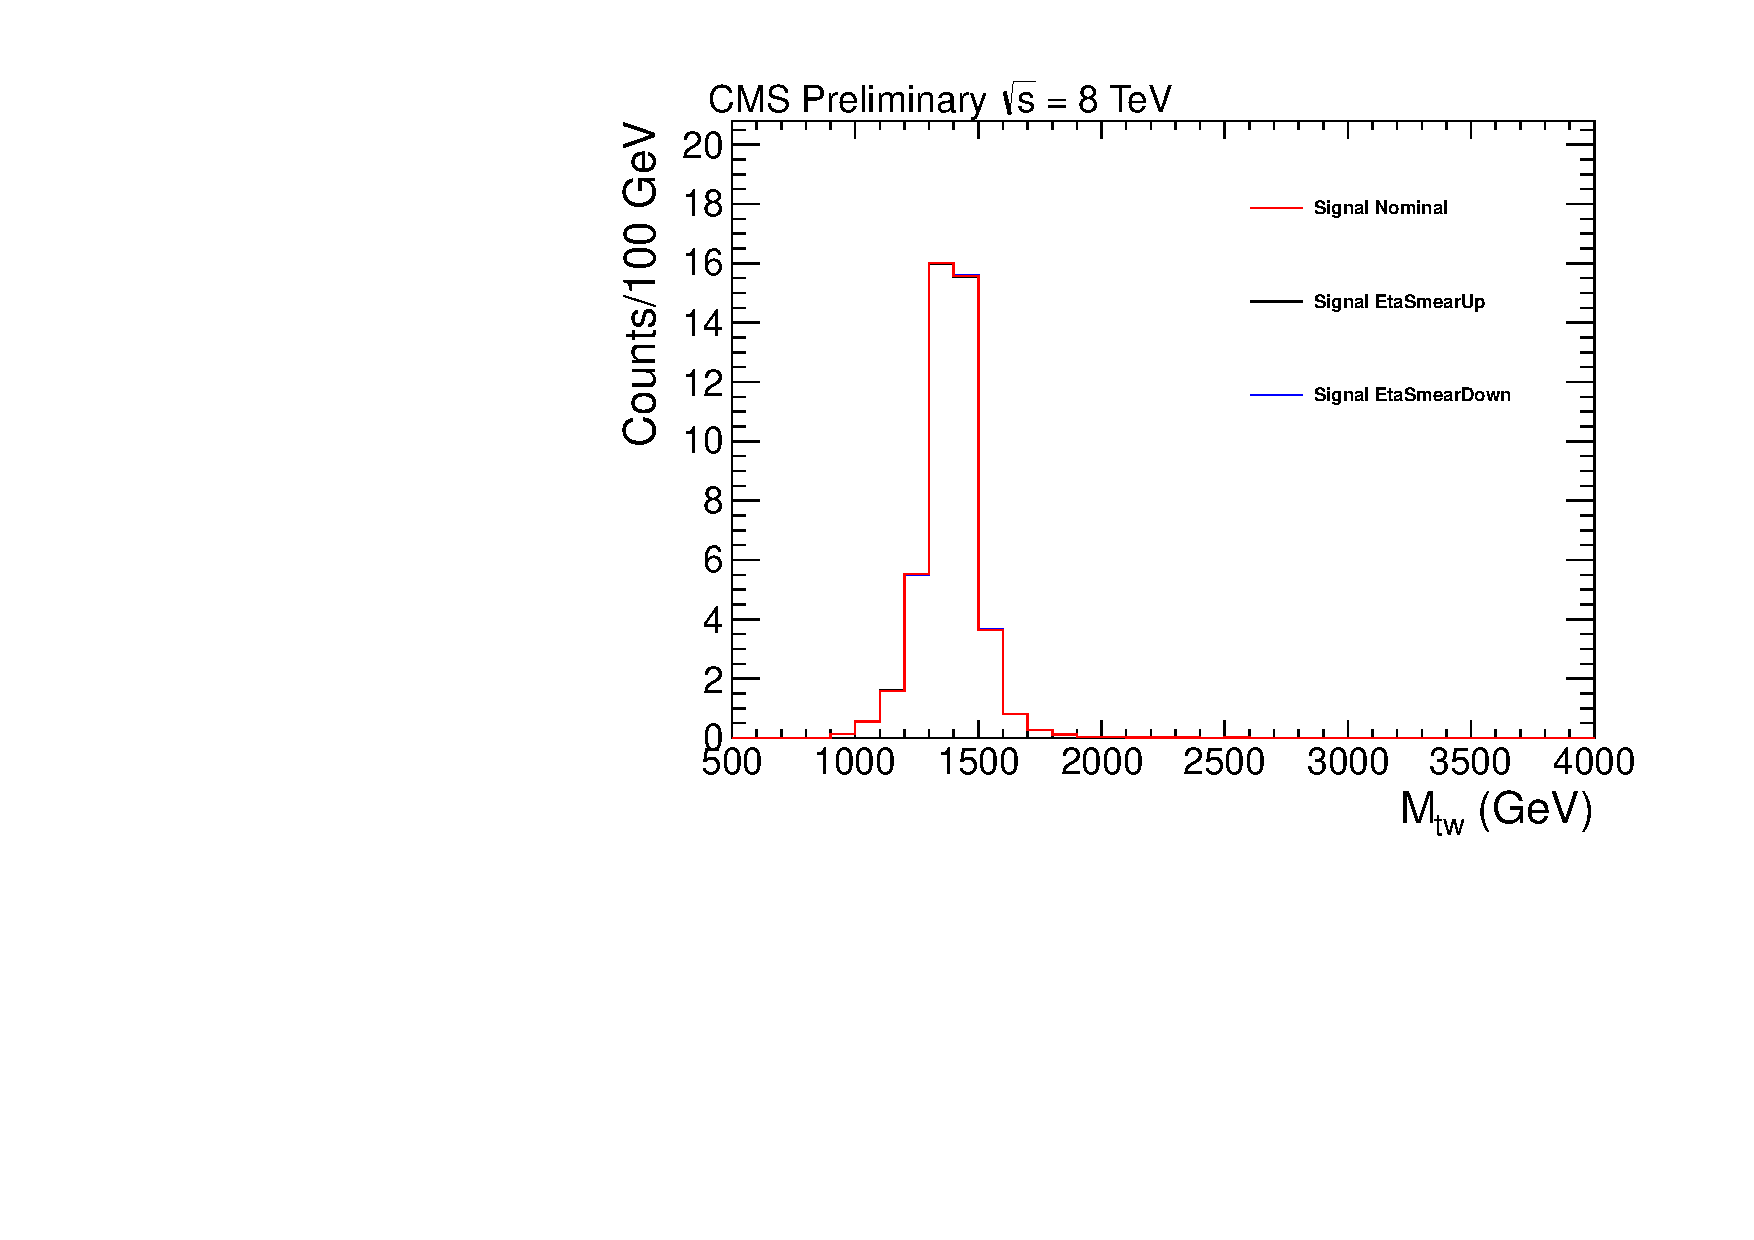
\includegraphics[width=0.45\textwidth]{AN-14-049/figs/Signal_M1400_EtaScaling}
\caption{
Jet Angular Resolution systematic variation for right-handed $\bs$  MC at the following mass points
(a) $\mathrm{M_{\bs}}$ = 1200$~\GeV$ 
(b) $\mathrm{M_{\bs}}$ = 1300$~\GeV$
(c) $\mathrm{M_{\bs}}$ = 1400$~\GeV$ 
}
\label{figs:bssignalJAR}
\end{center}
\end{figure}

\begin{figure}[htcb]
\begin{center}
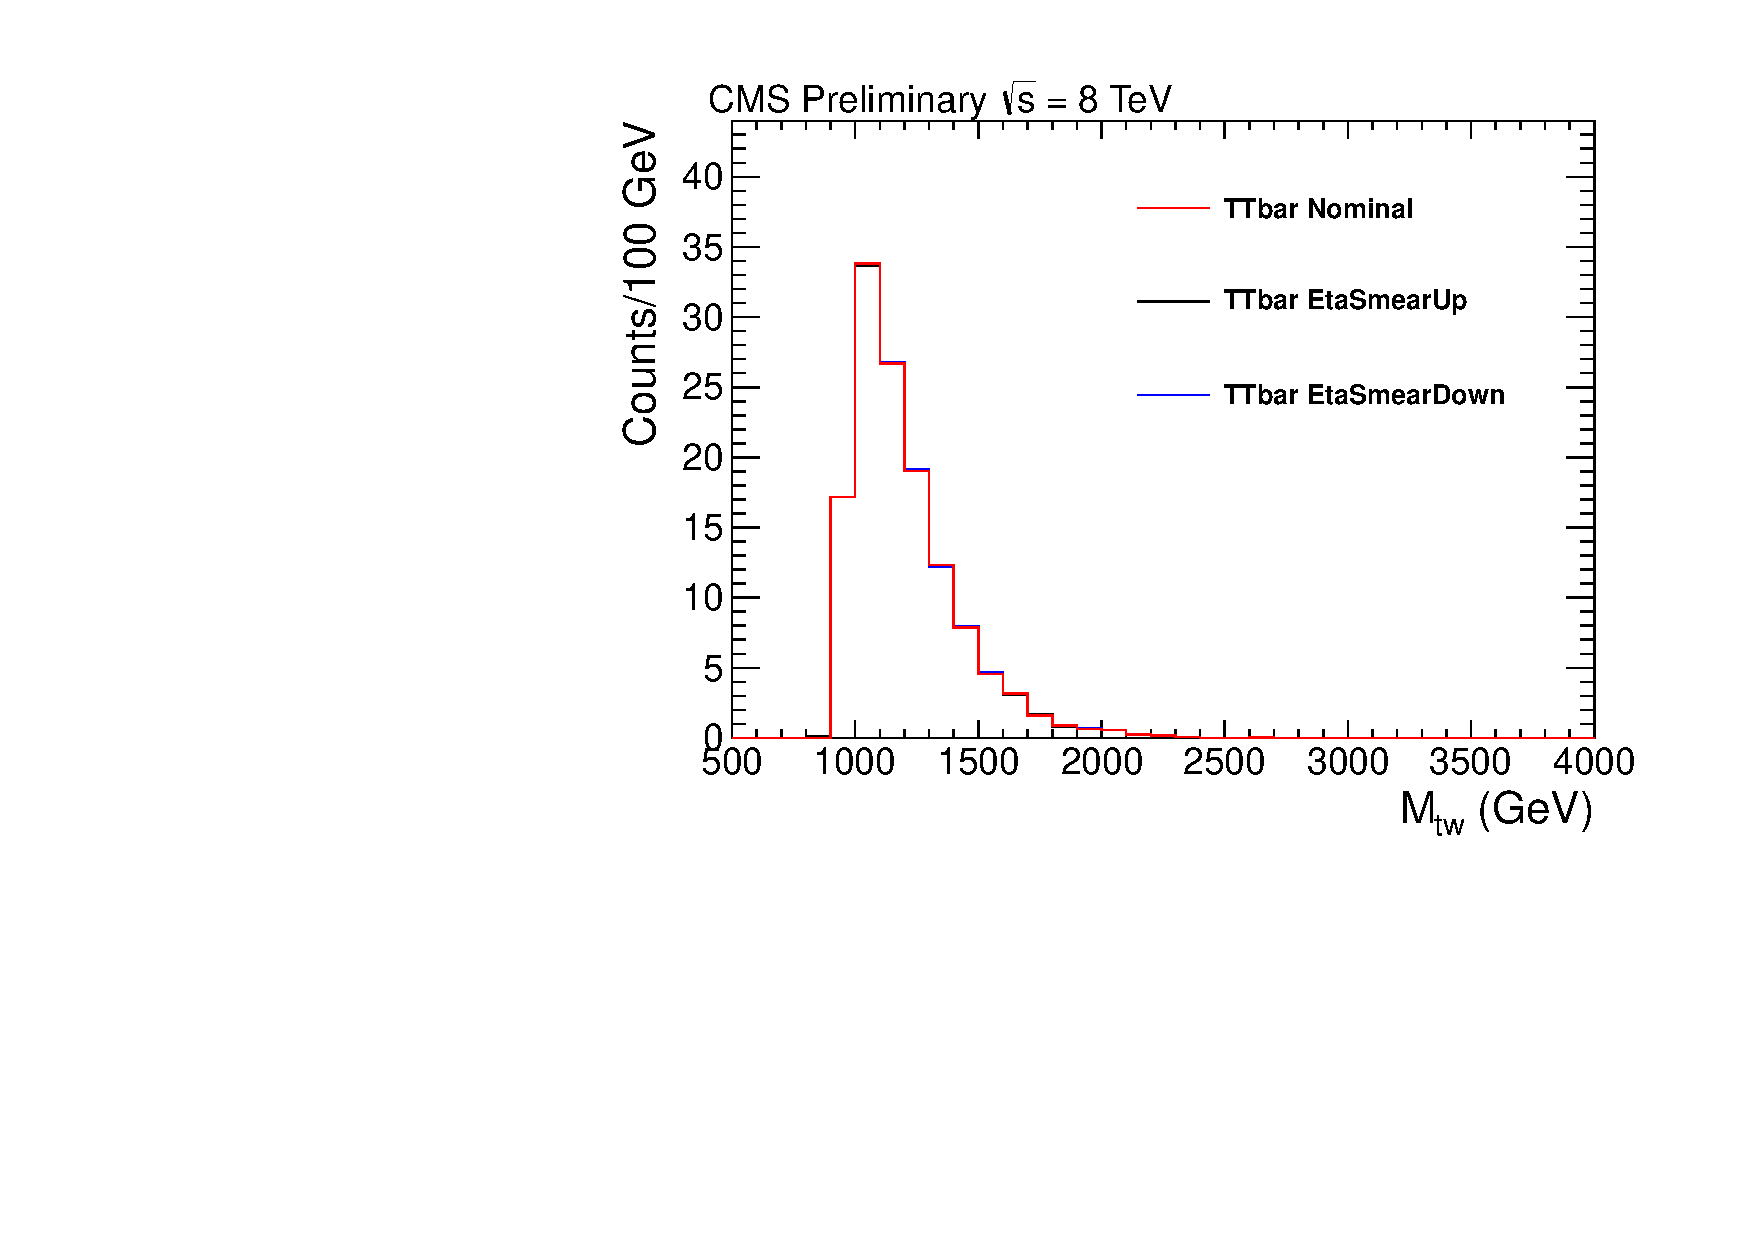
\includegraphics[width=0.7\textwidth]{AN-14-049/figs/TTbar_EtaScaling}
\caption{Jet Angular Resolution systematic variation for $\ttbar$ MC}
\label{figs:bsttbarJAR}
\end{center}
\end{figure}

\begin{figure}[htcb]
\begin{center}
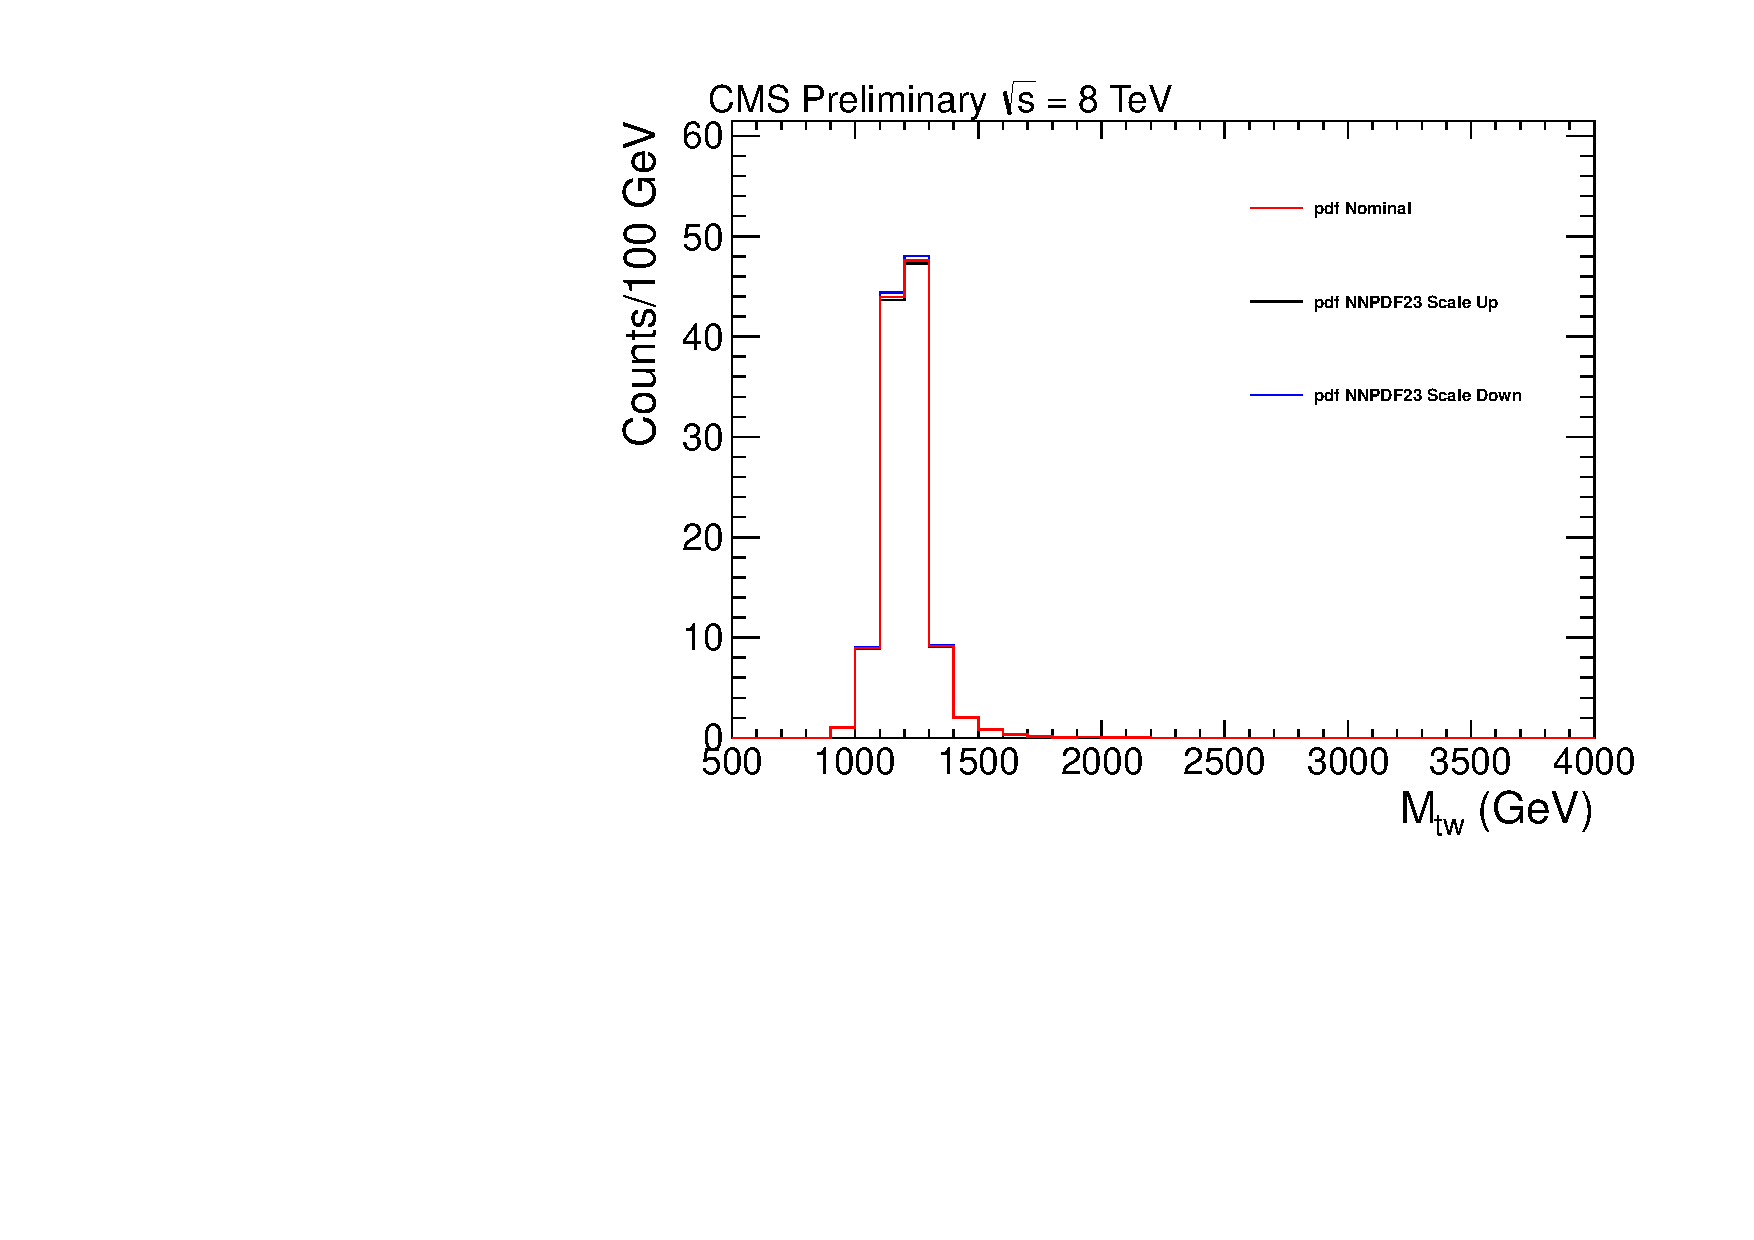
\includegraphics[width=0.45\textwidth]{AN-14-049/figs/Signal_M1200_PdfScaleNNPDF23.pdf}
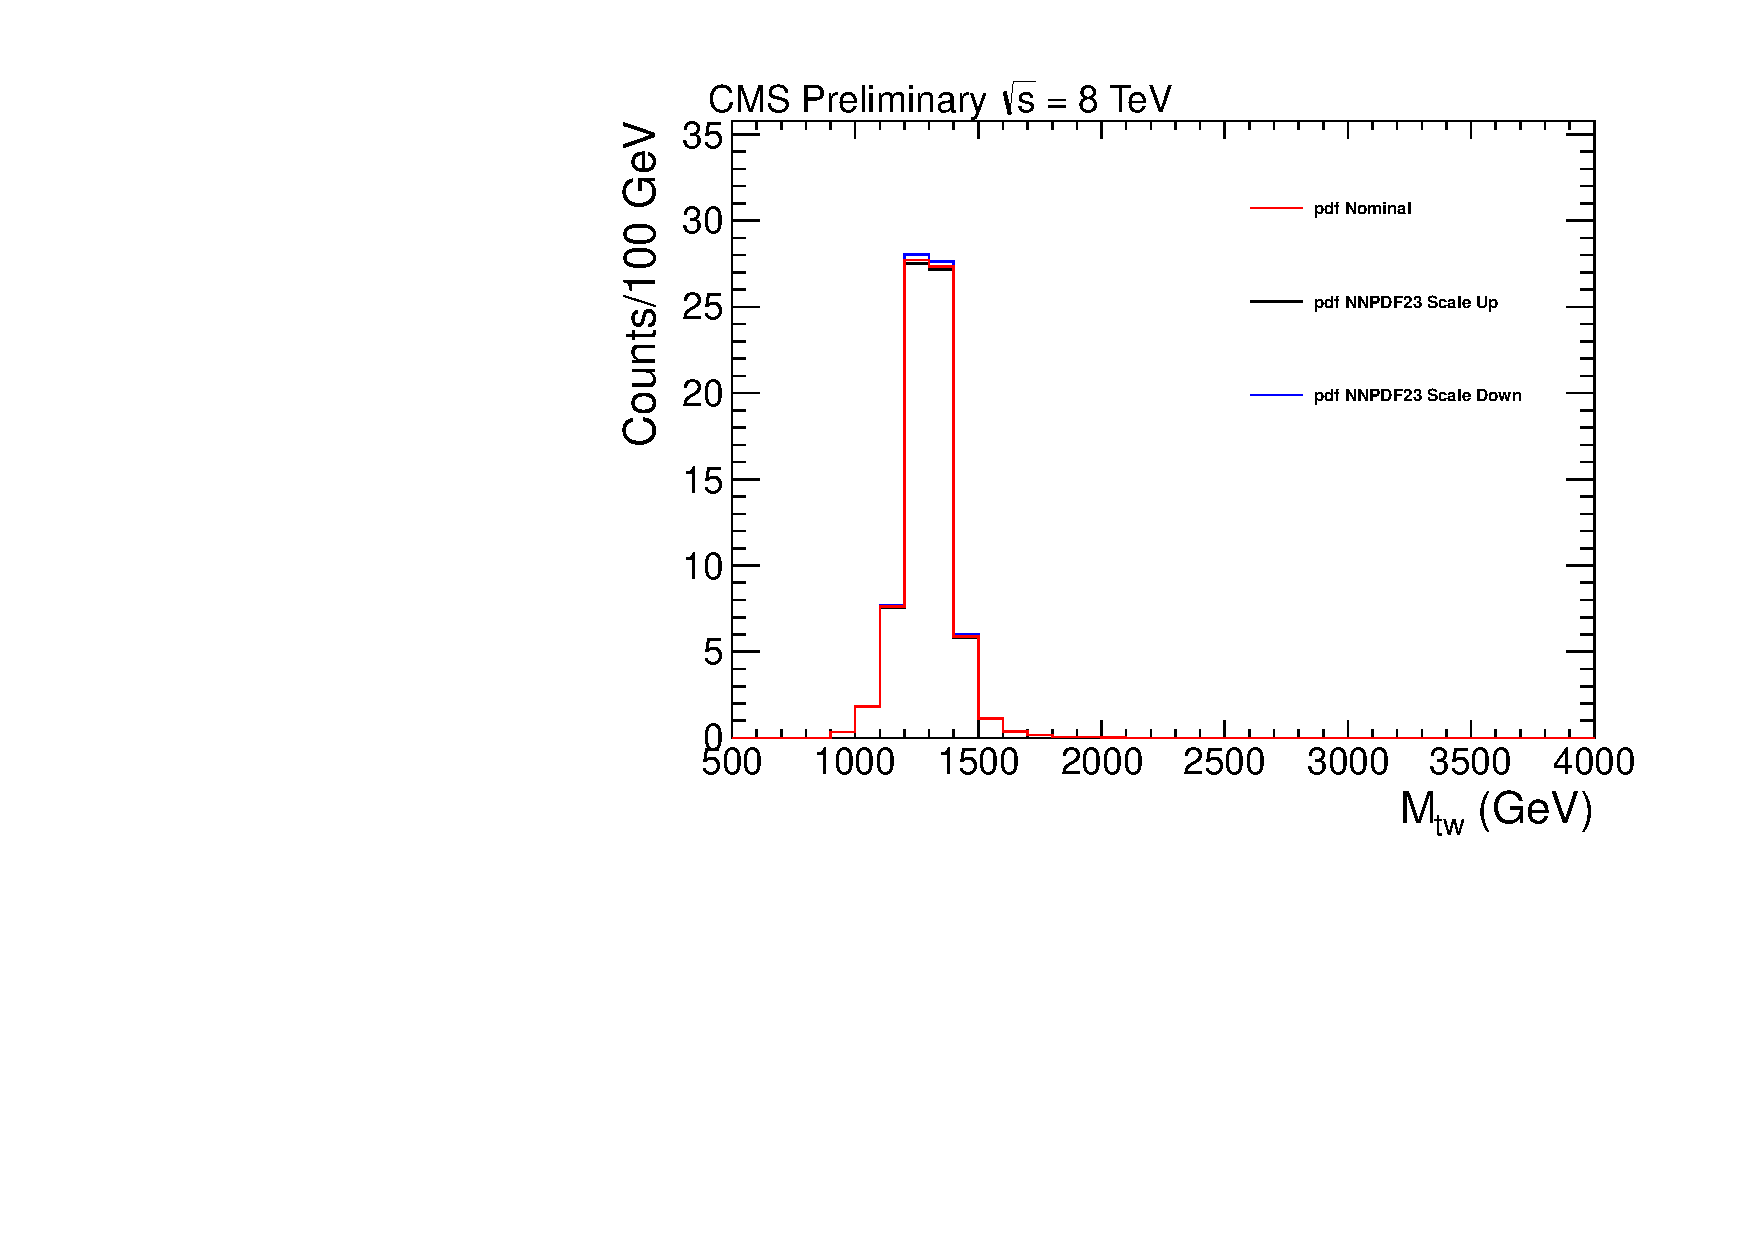
\includegraphics[width=0.45\textwidth]{AN-14-049/figs/Signal_M1300_PdfScaleNNPDF23.pdf}
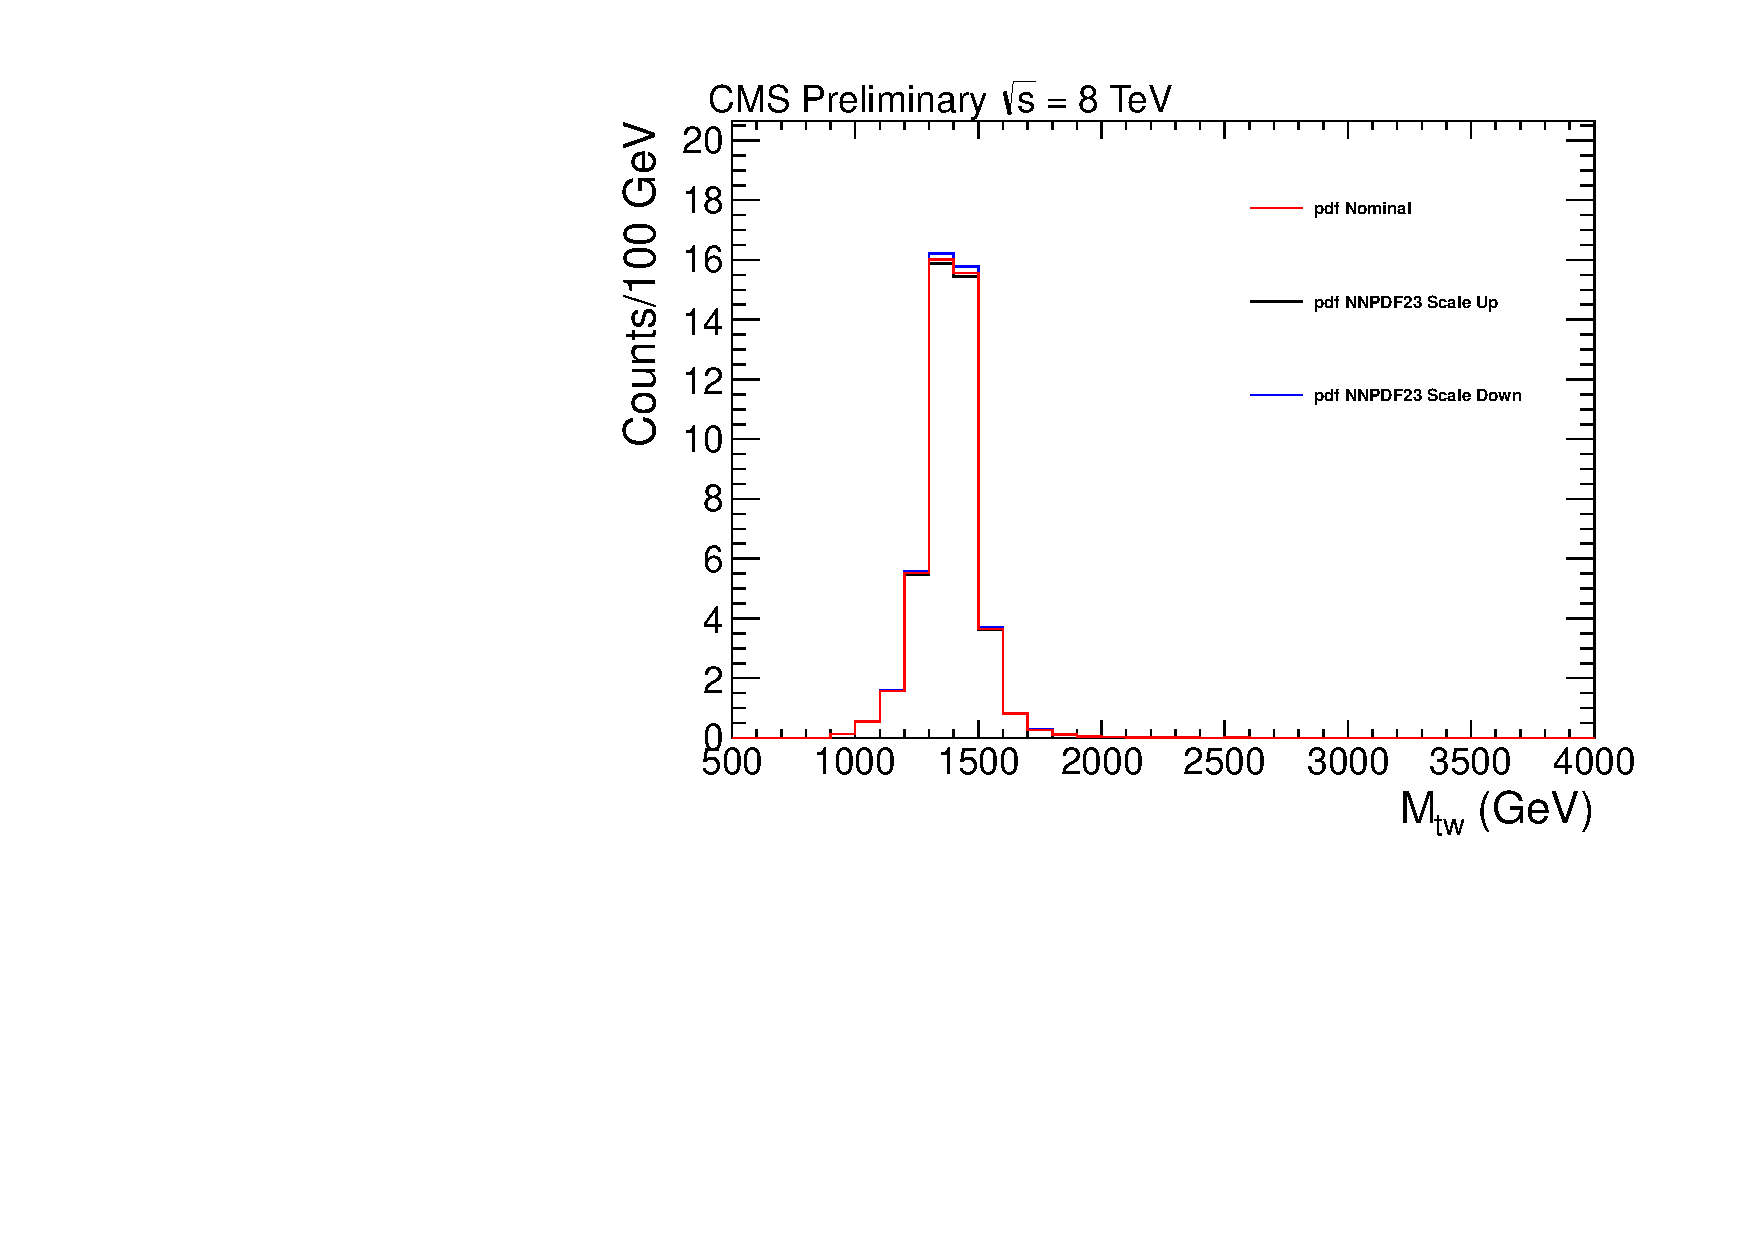
\includegraphics[width=0.45\textwidth]{AN-14-049/figs/Signal_M1400_PdfScaleNNPDF23.pdf}
\caption{
PDF systematic variation for right-handed $\bs$  MC at the following mass points
(a) $\mathrm{M_{\bs}}$ = 1200$~\GeV$ 
(b) $\mathrm{M_{\bs}}$ = 1300$~\GeV$
(c) $\mathrm{M_{\bs}}$ = 1400$~\GeV$ 
}
\label{figs:bssignalPDF}
\end{center}
\end{figure}

\begin{figure}[htcb]
\begin{center}
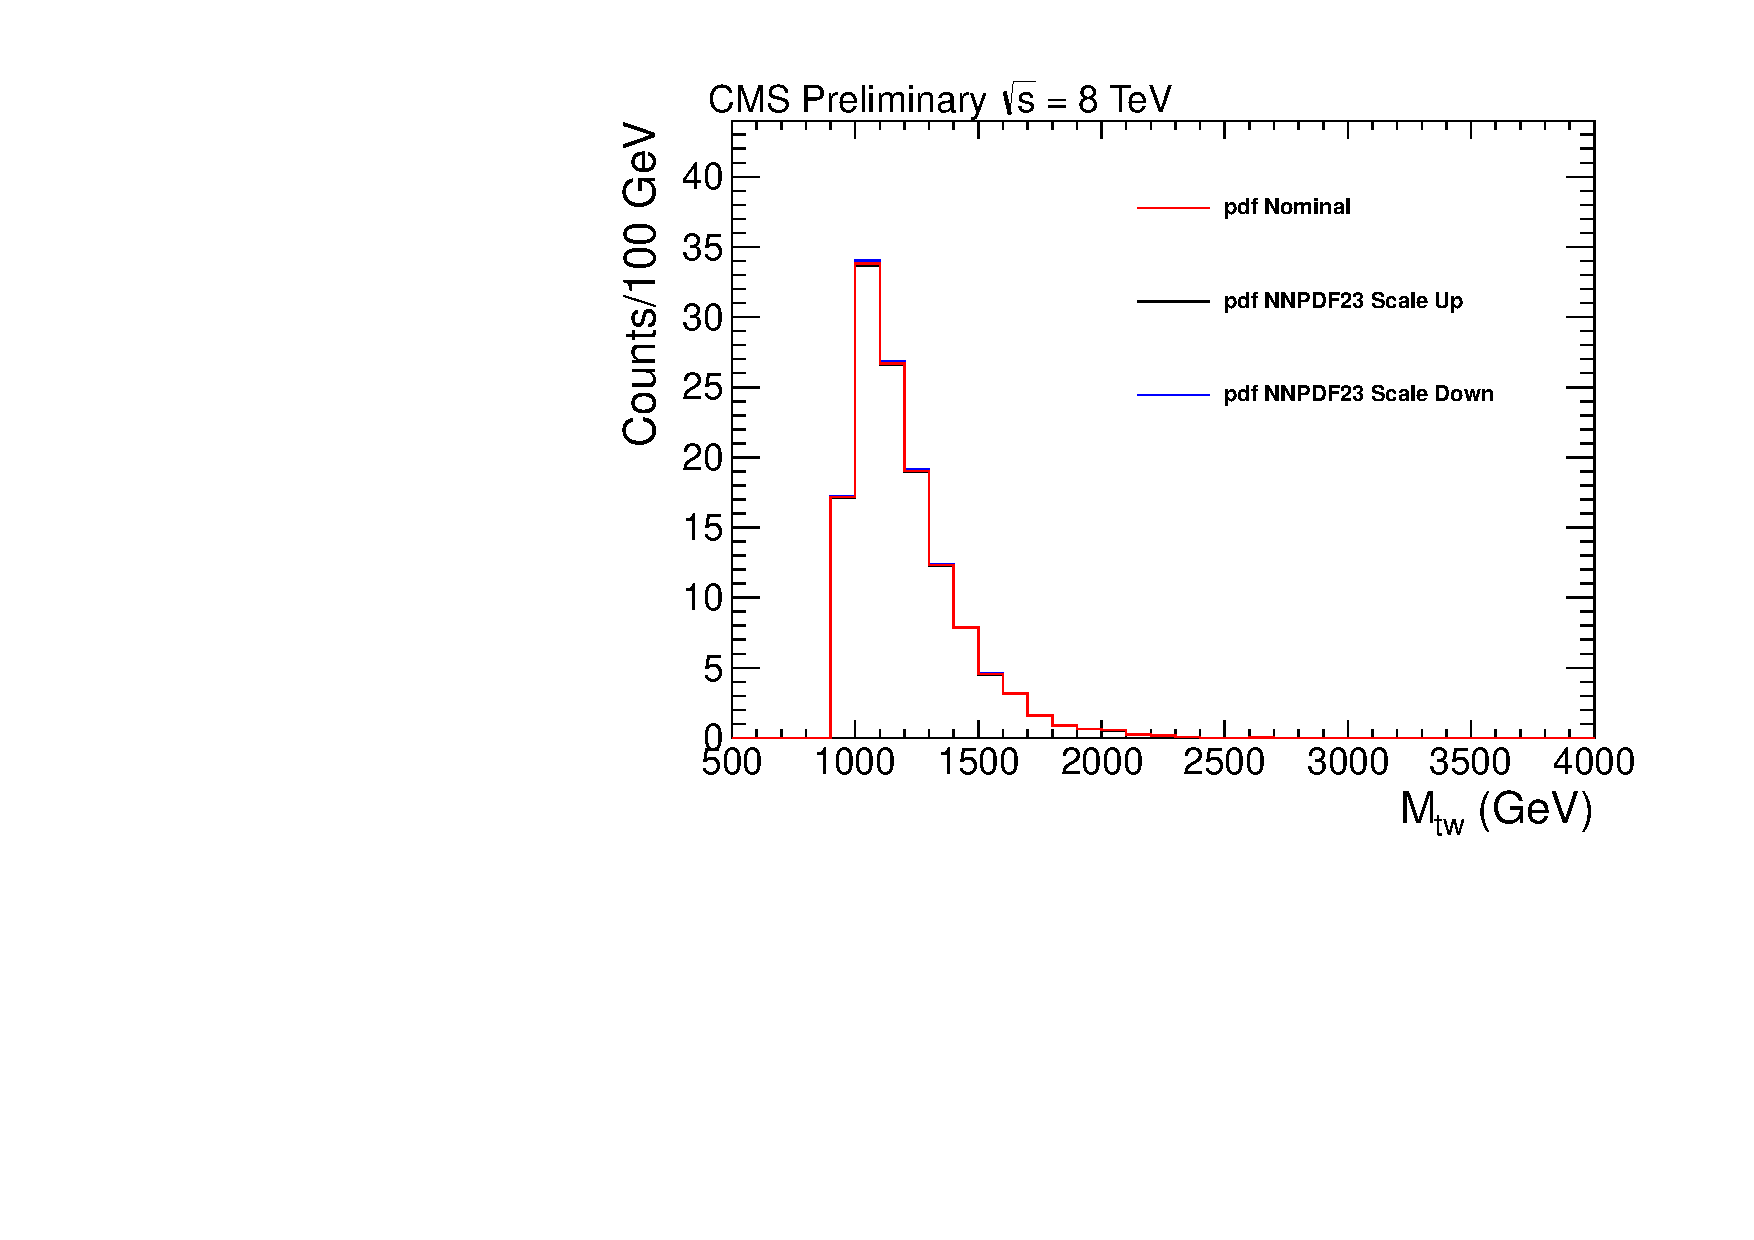
\includegraphics[width=0.7\textwidth]{AN-14-049/figs/TTbar_PdfScaleNNPDF23.pdf}
\caption{PDF systematic variation for $\ttbar$ MC}
\label{figs:bsttbarPDF}
\end{center}
\end{figure}

\begin{figure}[htcb]
\begin{center}
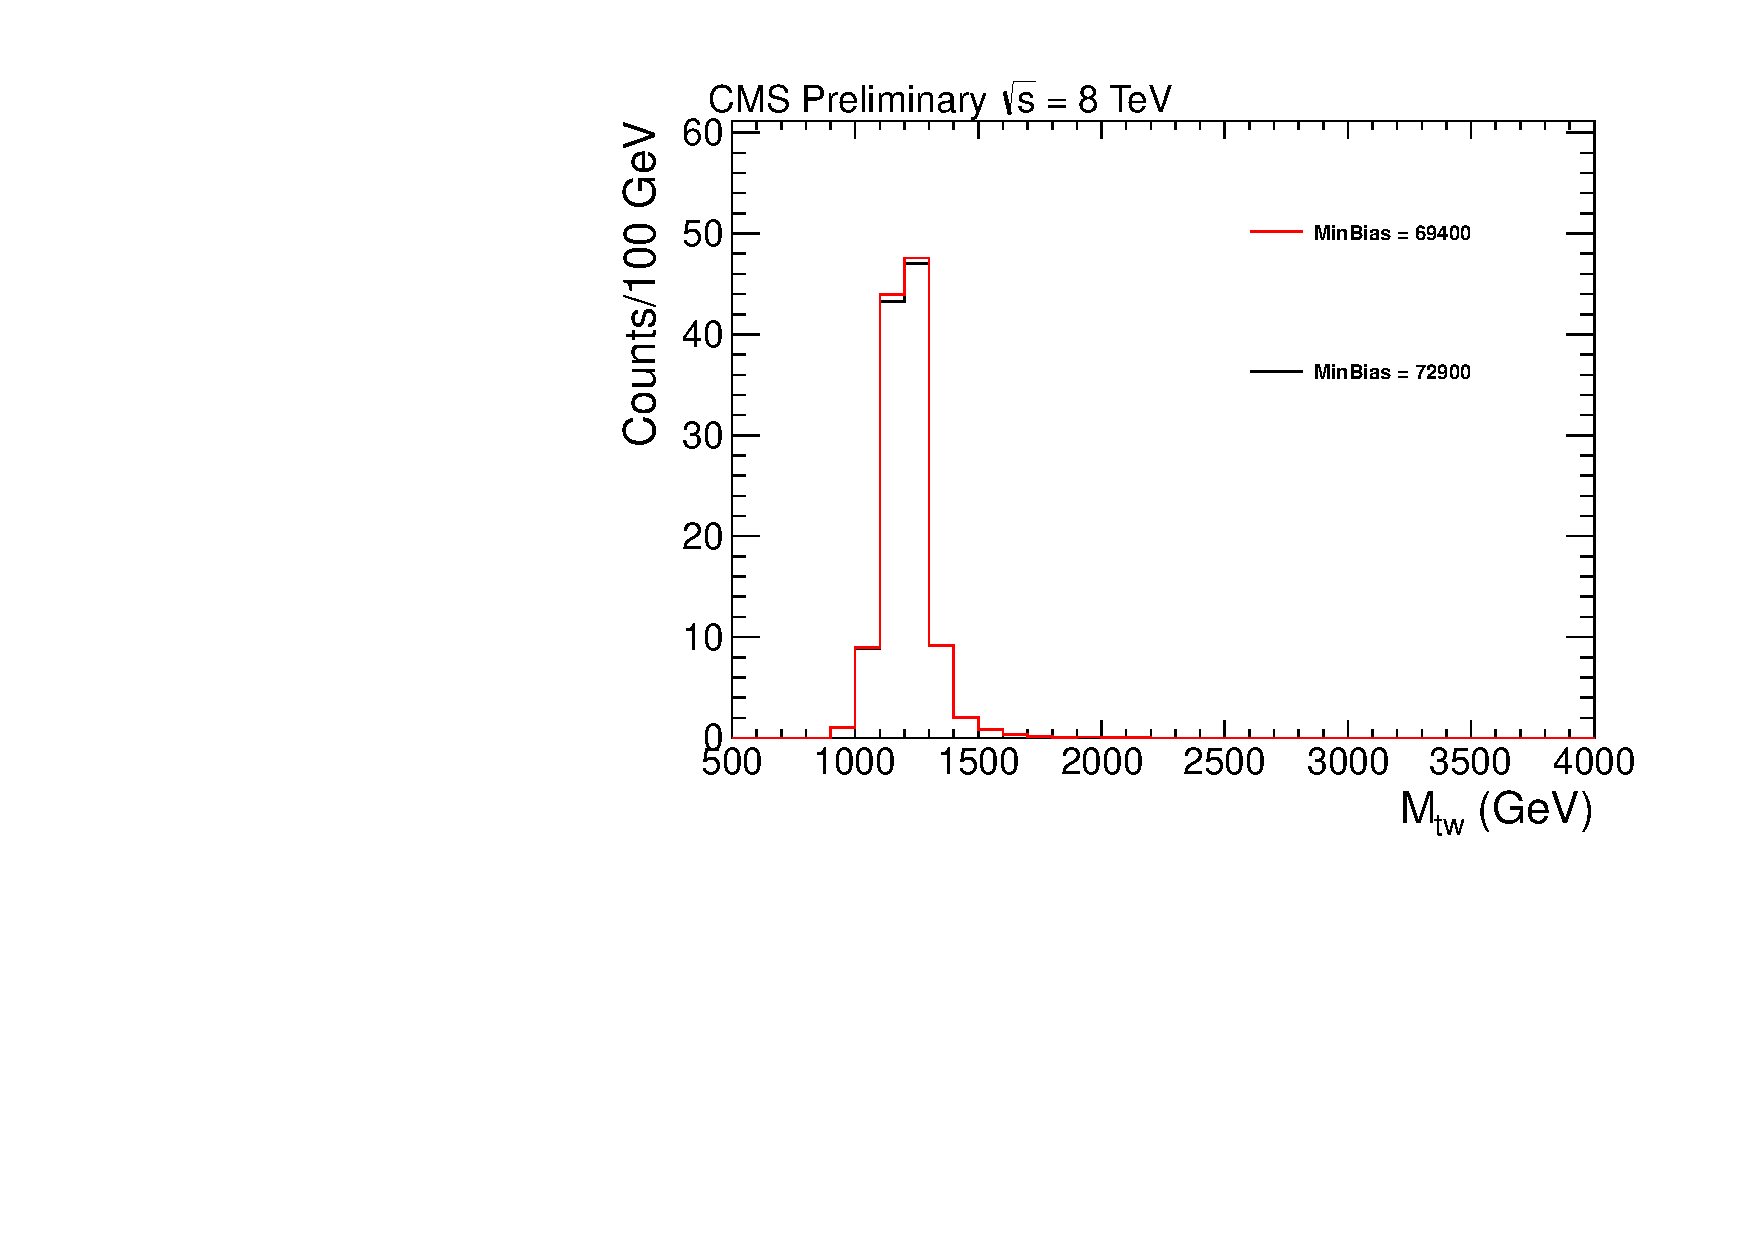
\includegraphics[width=0.45\textwidth]{AN-14-049/figs/Signal_M1200_PileupReweighting.pdf}
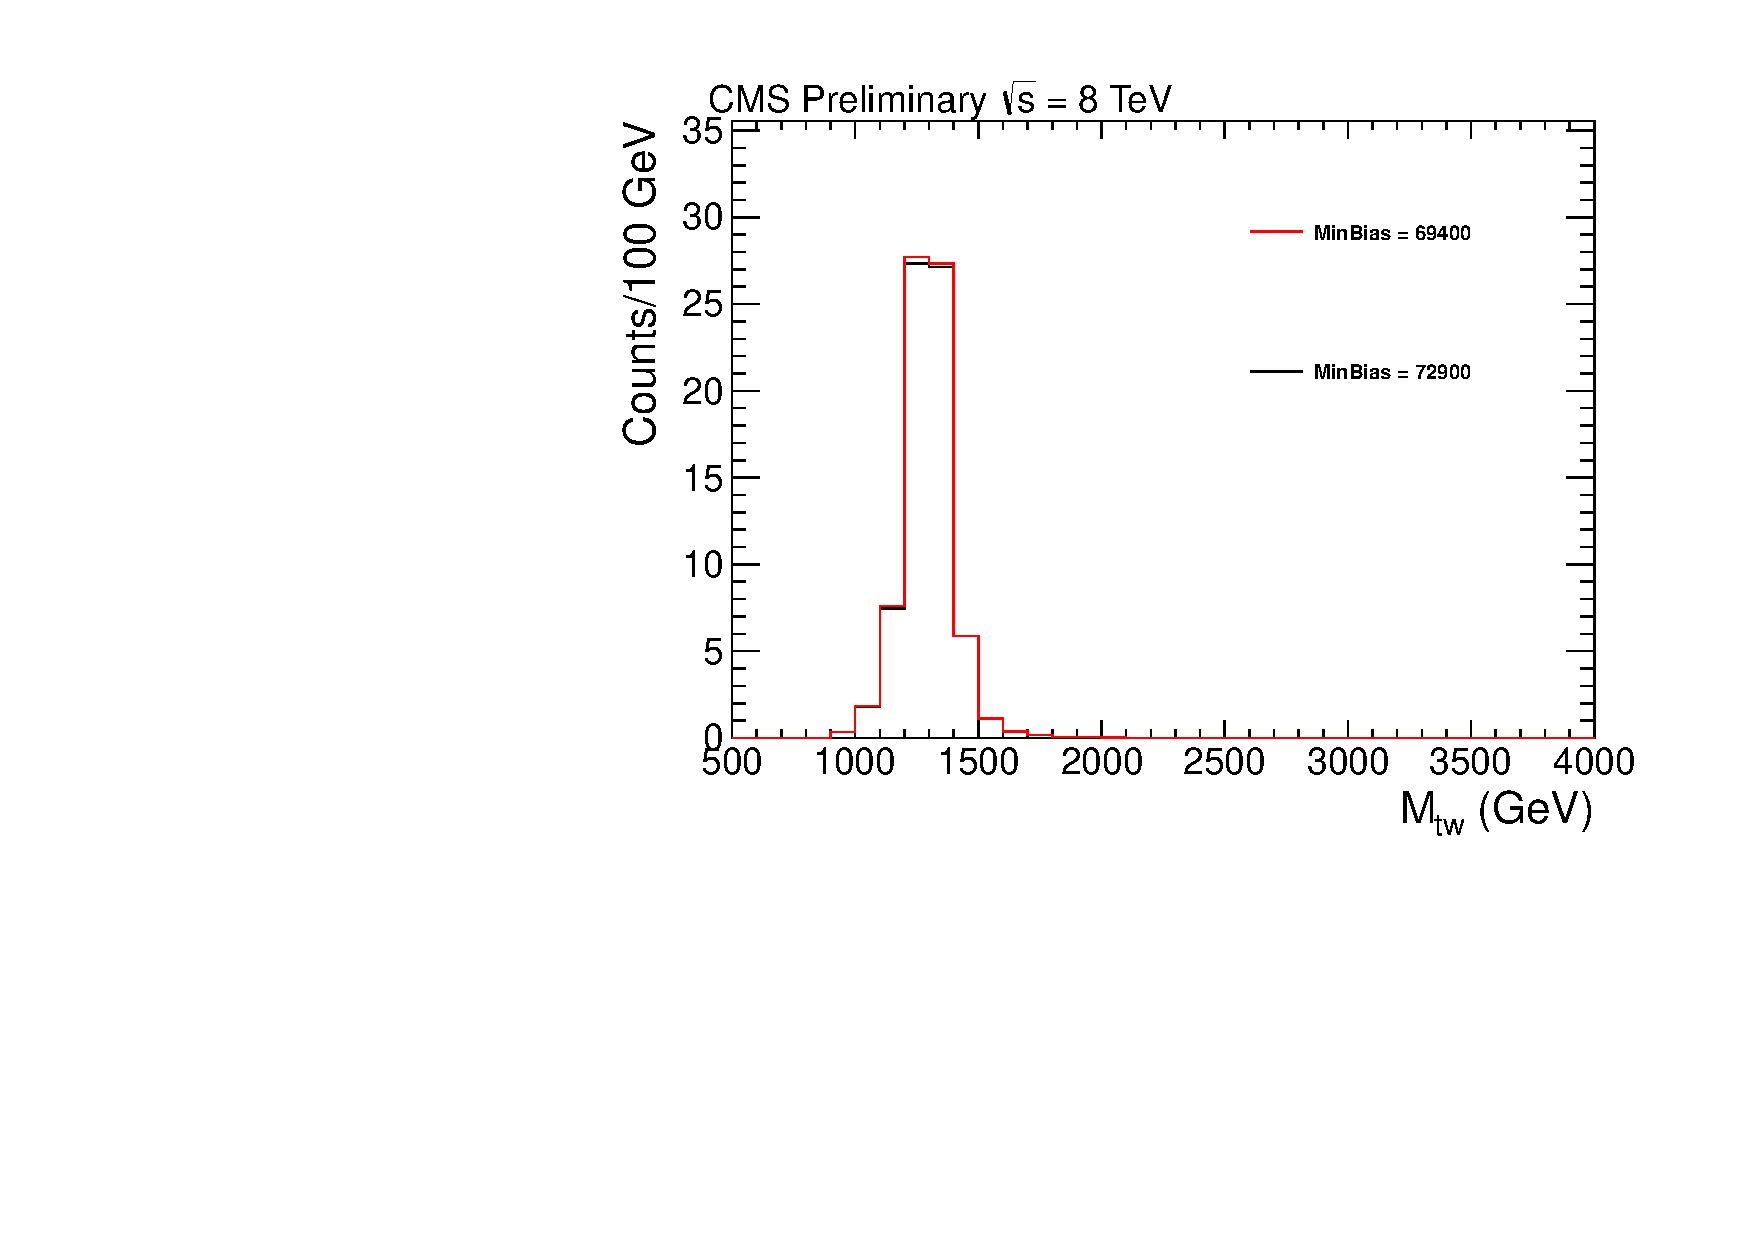
\includegraphics[width=0.45\textwidth]{AN-14-049/figs/Signal_M1300_PileupReweighting.pdf}
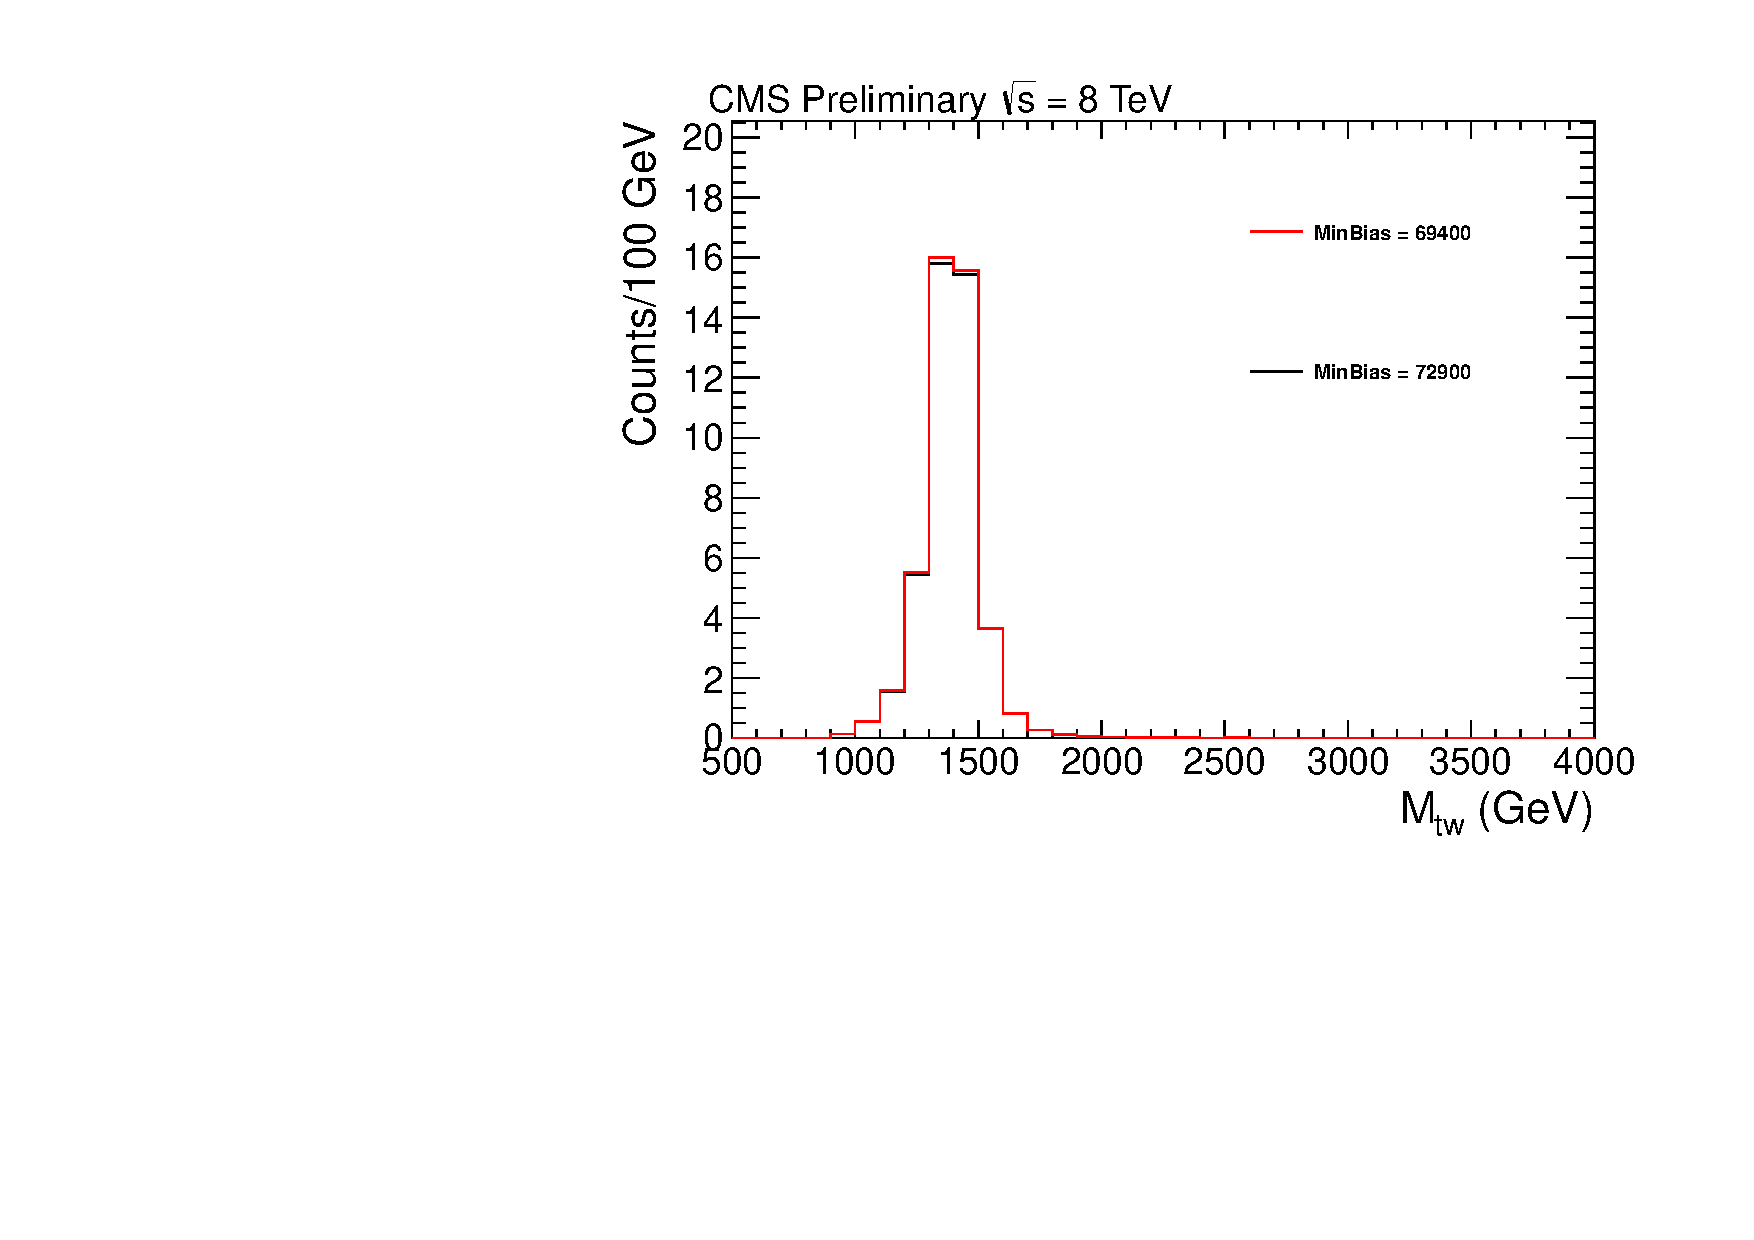
\includegraphics[width=0.45\textwidth]{AN-14-049/figs/Signal_M1400_PileupReweighting.pdf}
\caption{
Pileup systematic variation for right-handed $\bs$  MC at the following mass points
(a) $\mathrm{M_{\bs}}$ = 1200$~\GeV$ 
(b) $\mathrm{M_{\bs}}$ = 1300$~\GeV$
(c) $\mathrm{M_{\bs}}$ = 1400$~\GeV$ 
}
\label{figs:bssignalPU}
\end{center}
\end{figure}

%\begin{figure}[htcb]
%\begin{center}
%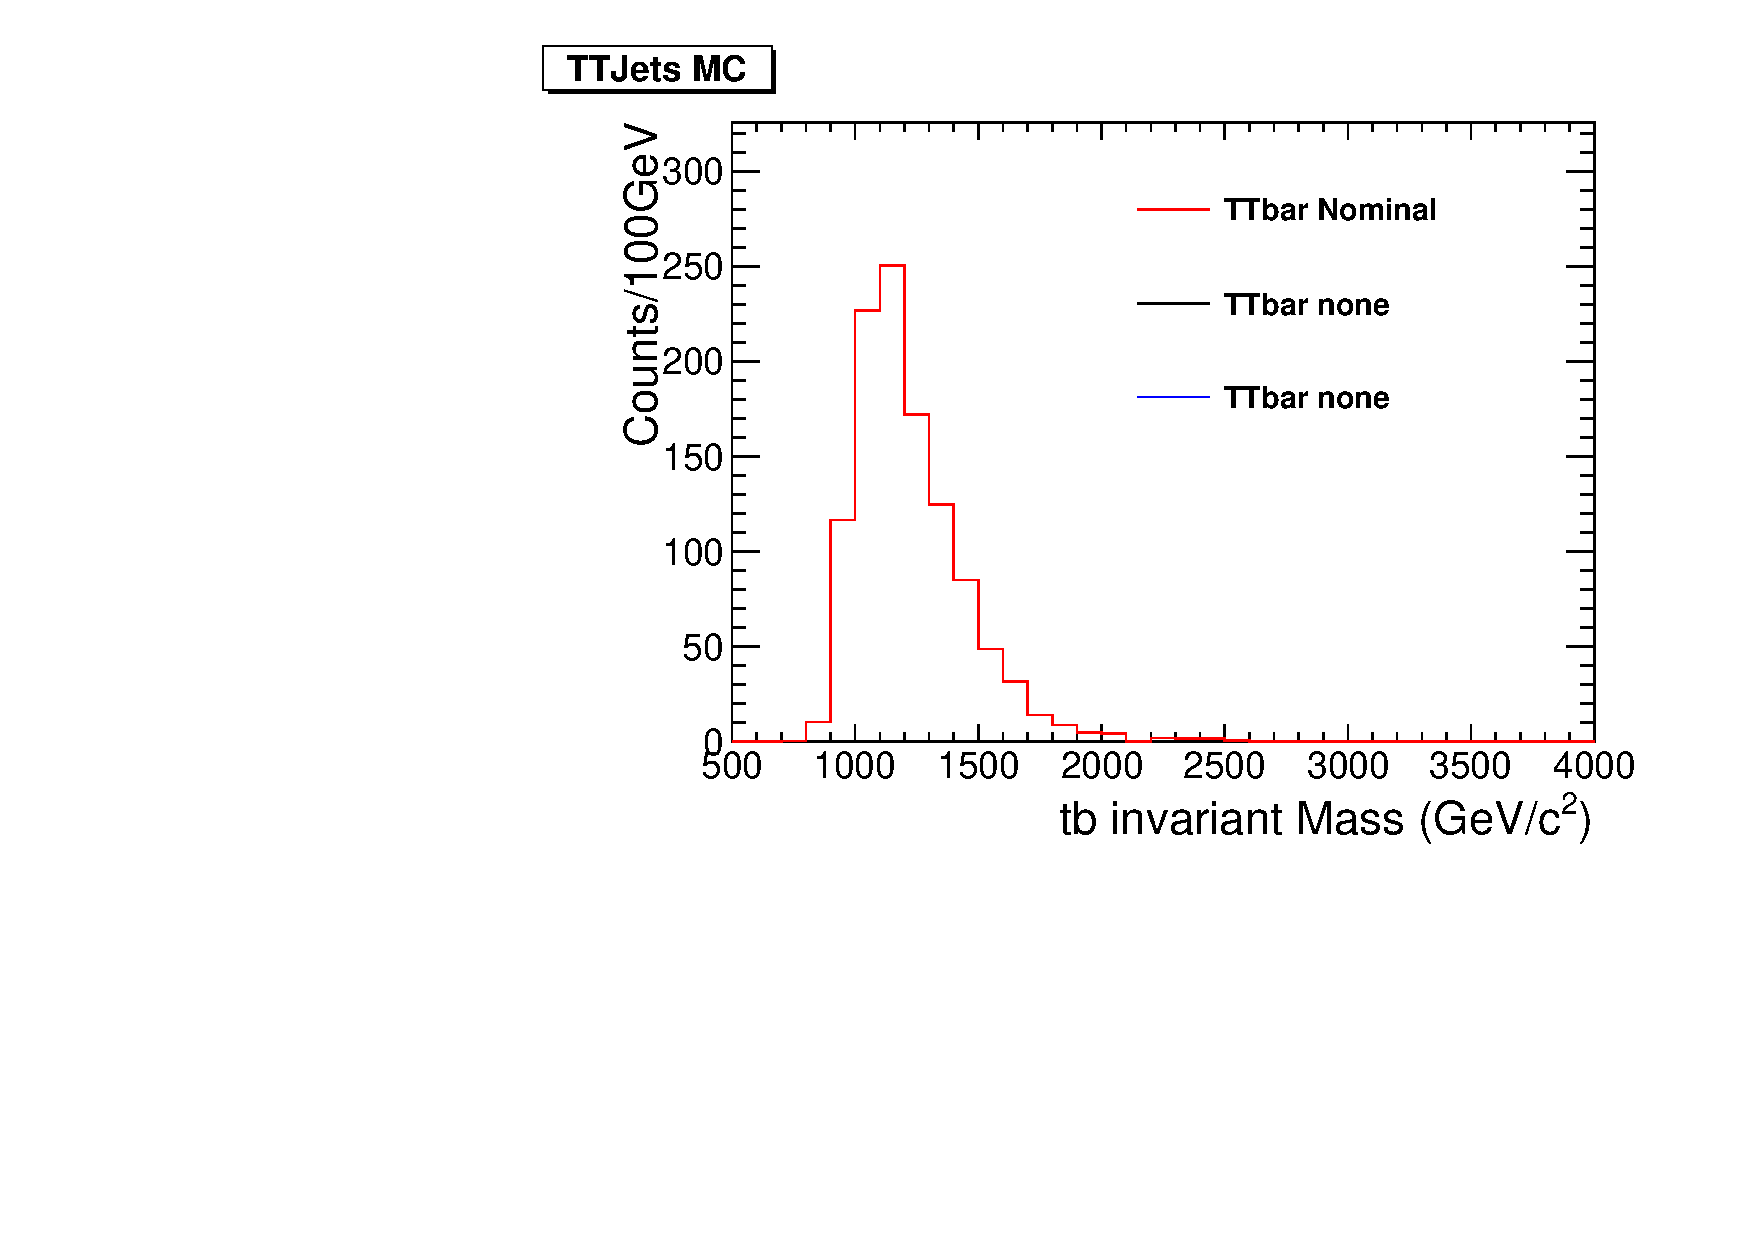
\includegraphics[width=0.7\textwidth]{AN-14-049/figs/TTbar_PileupReweighting}
%\caption{Pileup systematic variation for $\ttbar$ MC}
%\label{figs:bsttbarPU}
%\end{center}
%\end{figure}

\begin{figure}[htcb]
\begin{center}
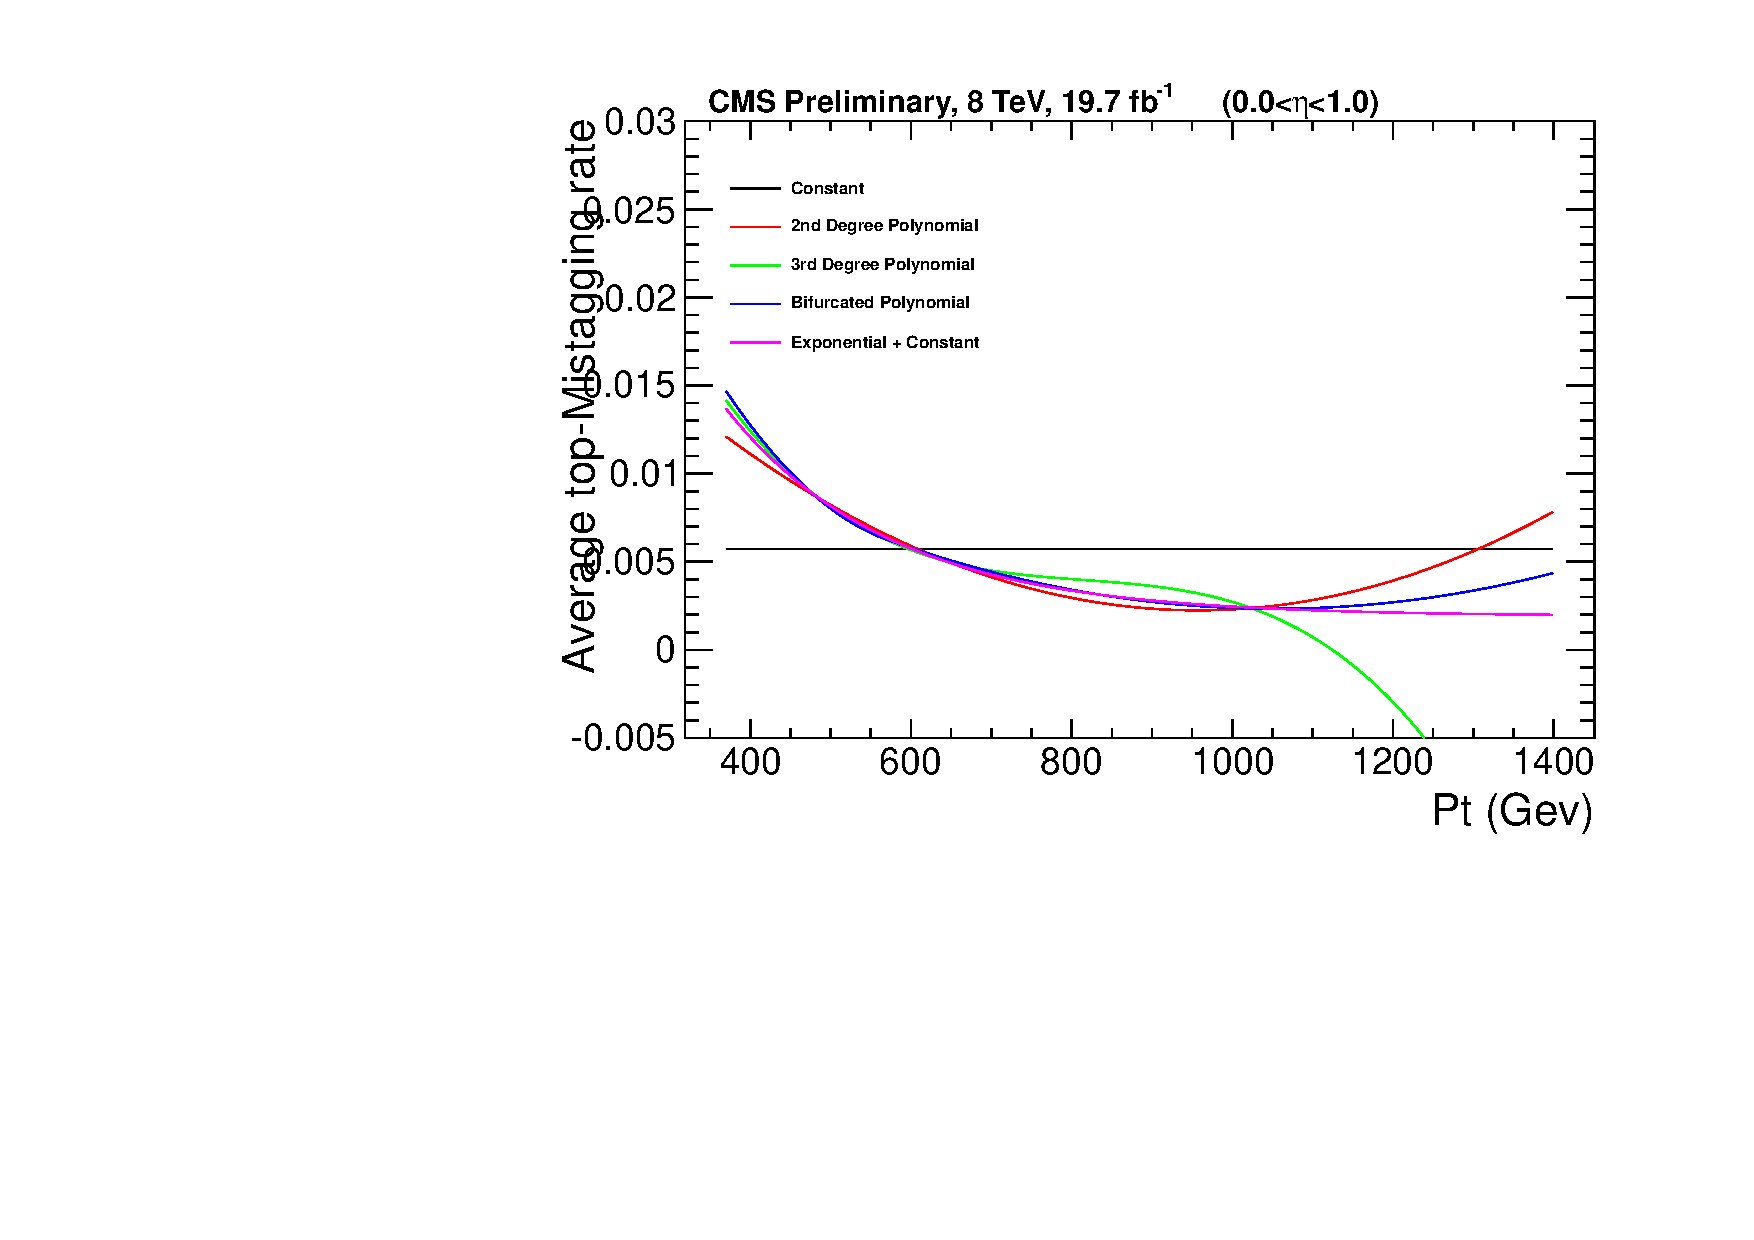
\includegraphics[width=0.7\textwidth]{AN-14-049/figs/BKGFITCOMPLOGE1.pdf}\\
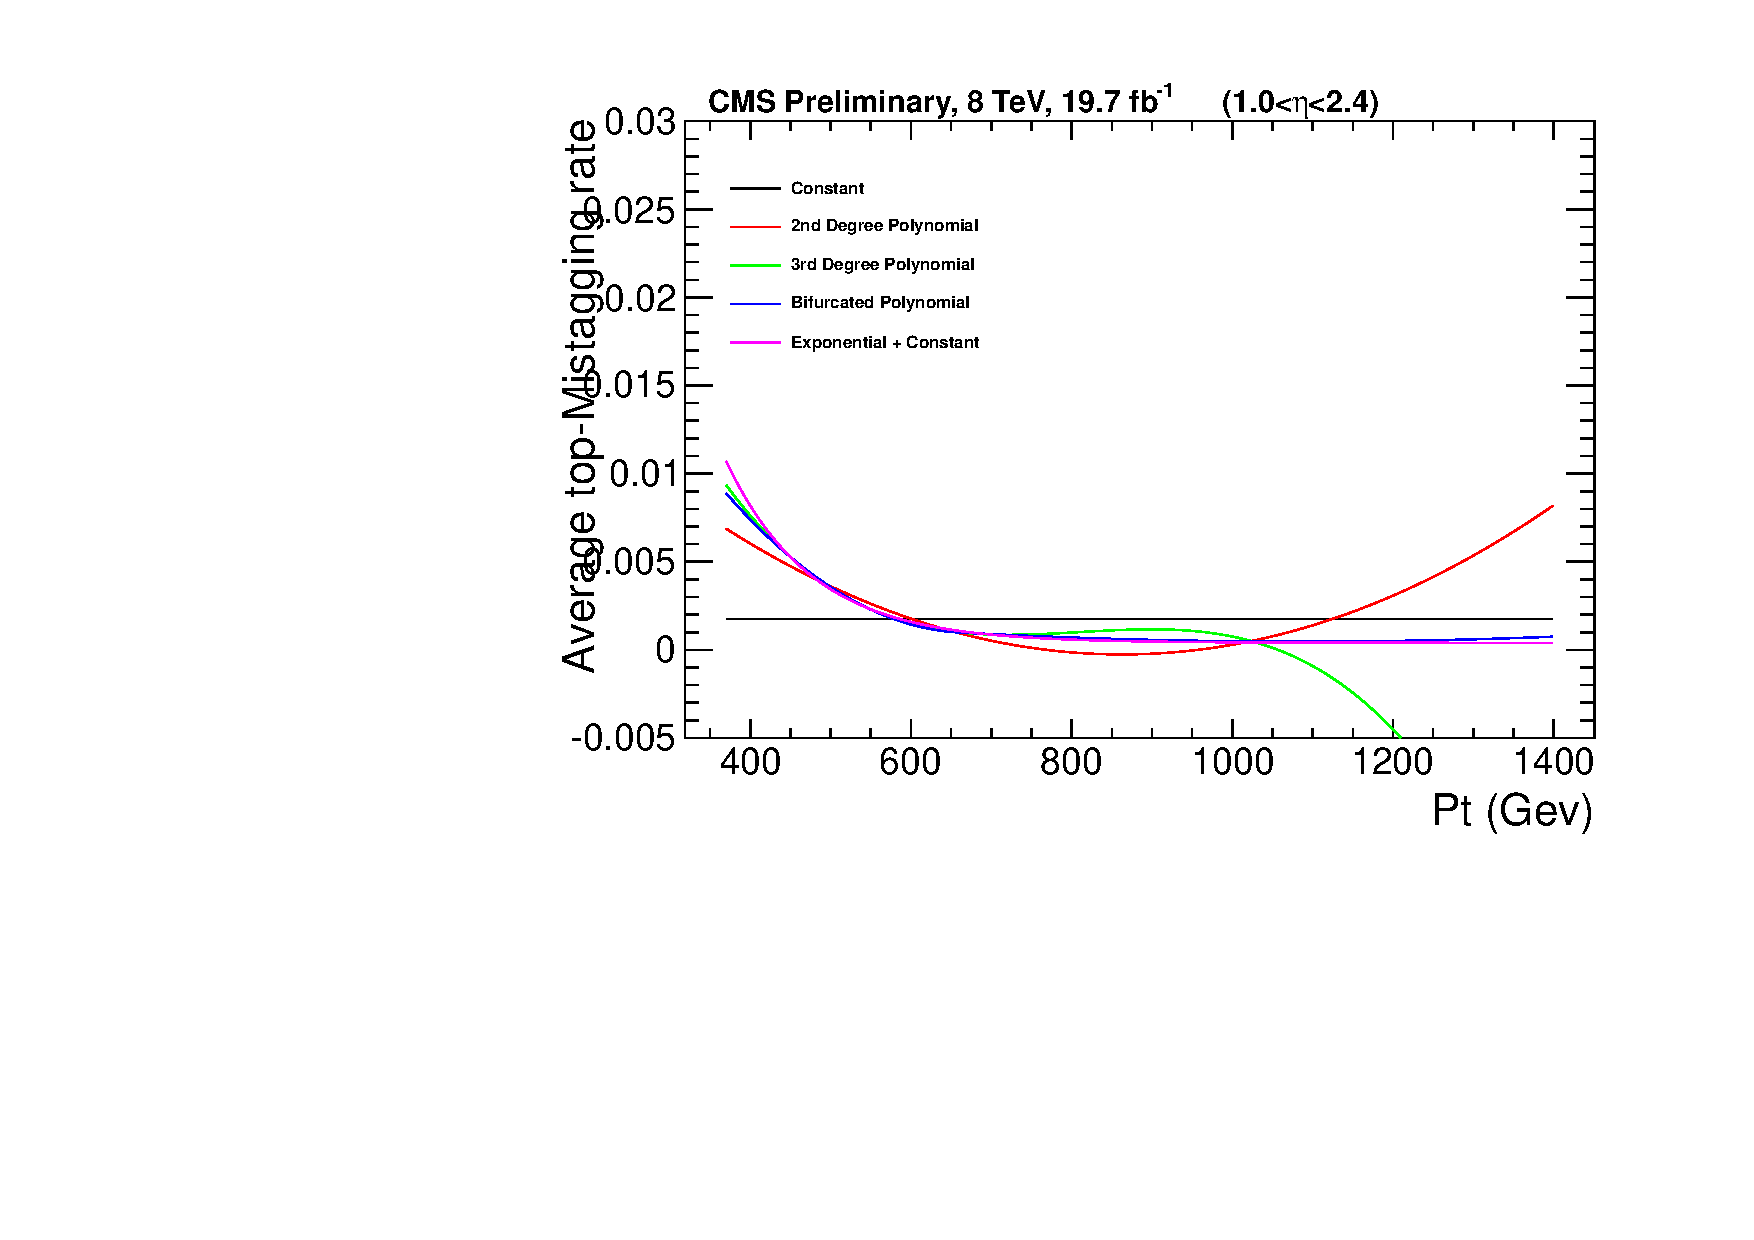
\includegraphics[width=0.7\textwidth]{AN-14-049/figs/BKGFITCOMPLOGE2.pdf}
\caption{
Alternative fit functions for the top-mistagging rate in $\eta$ regions
(a) Low
(b) High
}
\label{figs:bsBKGFITCOMP}
\end{center}
\end{figure}

\begin{figure}[htcb]
\begin{center}
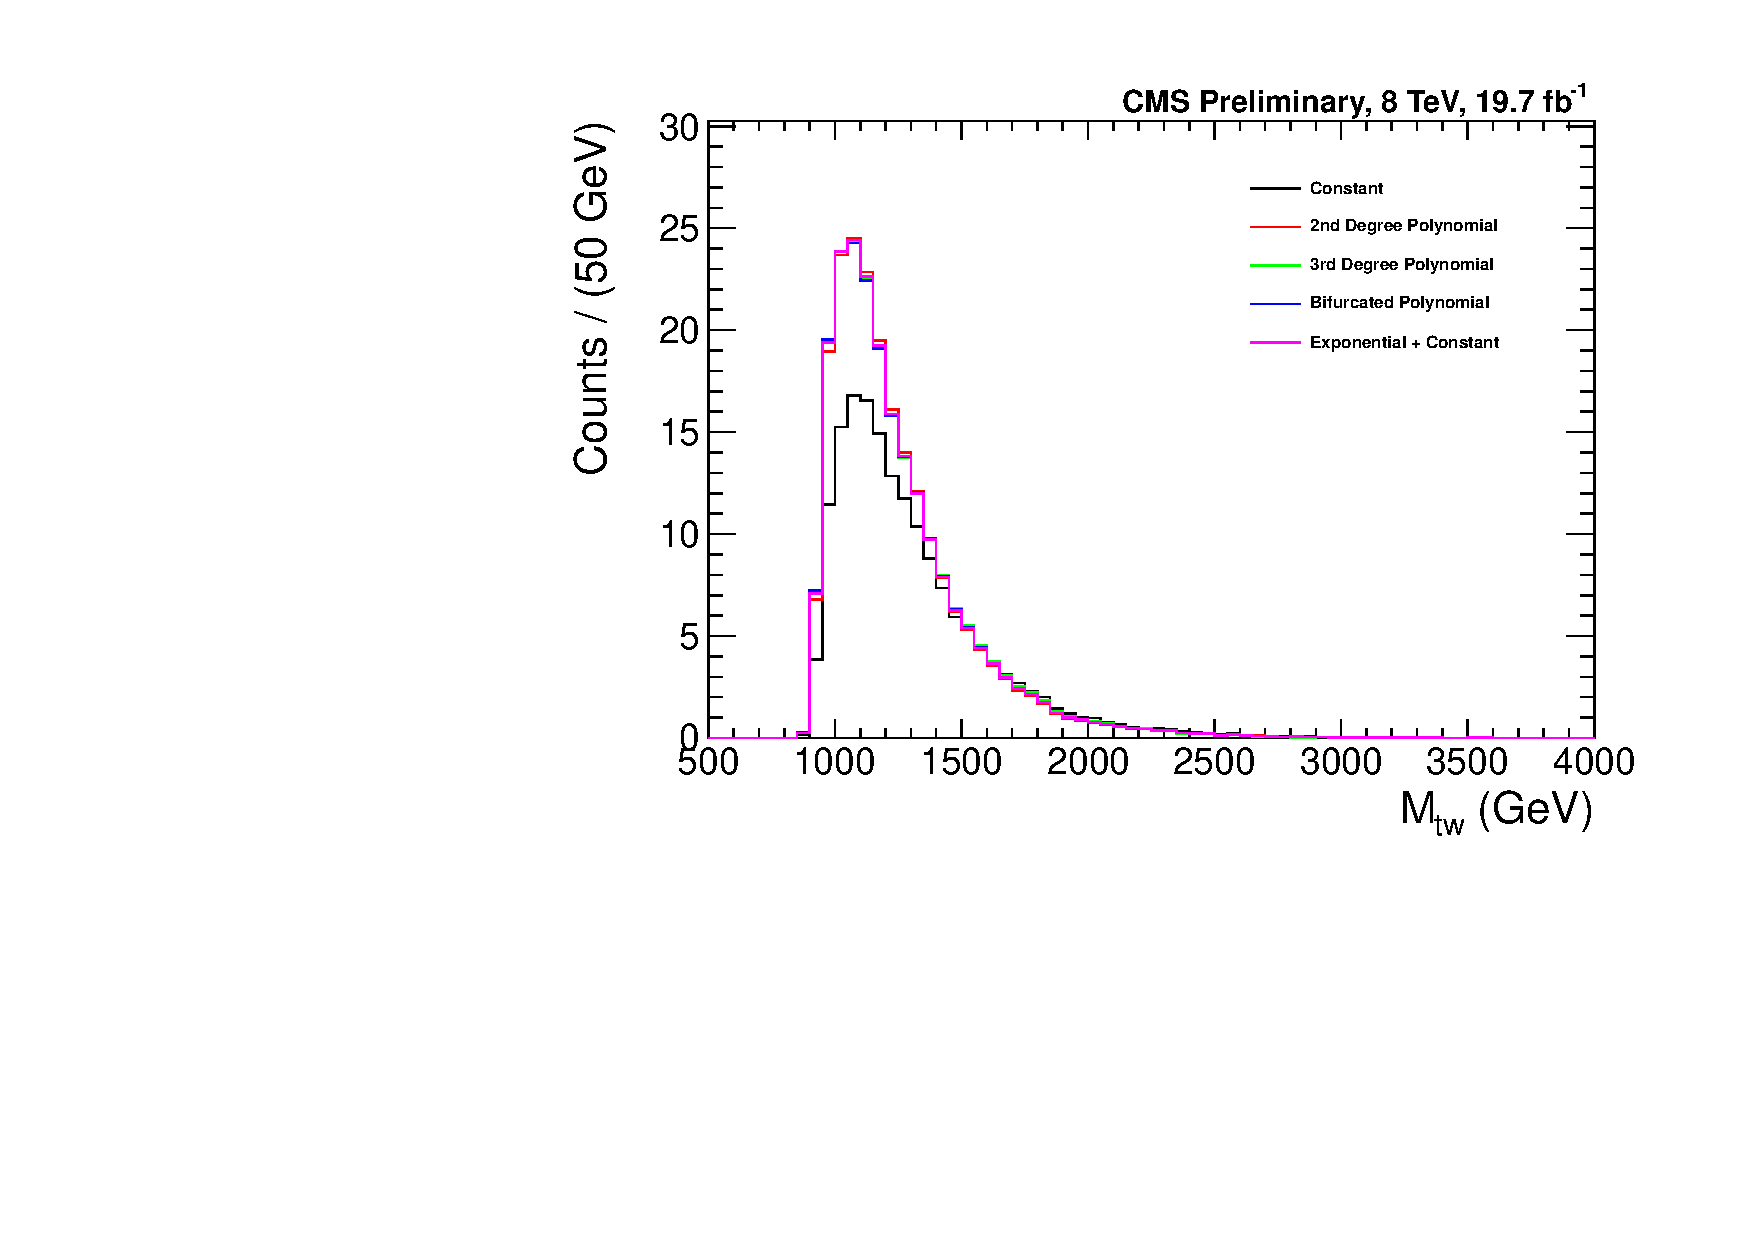
\includegraphics[width=0.7\textwidth]{AN-14-049/figs/BKGCOMP.pdf}\\
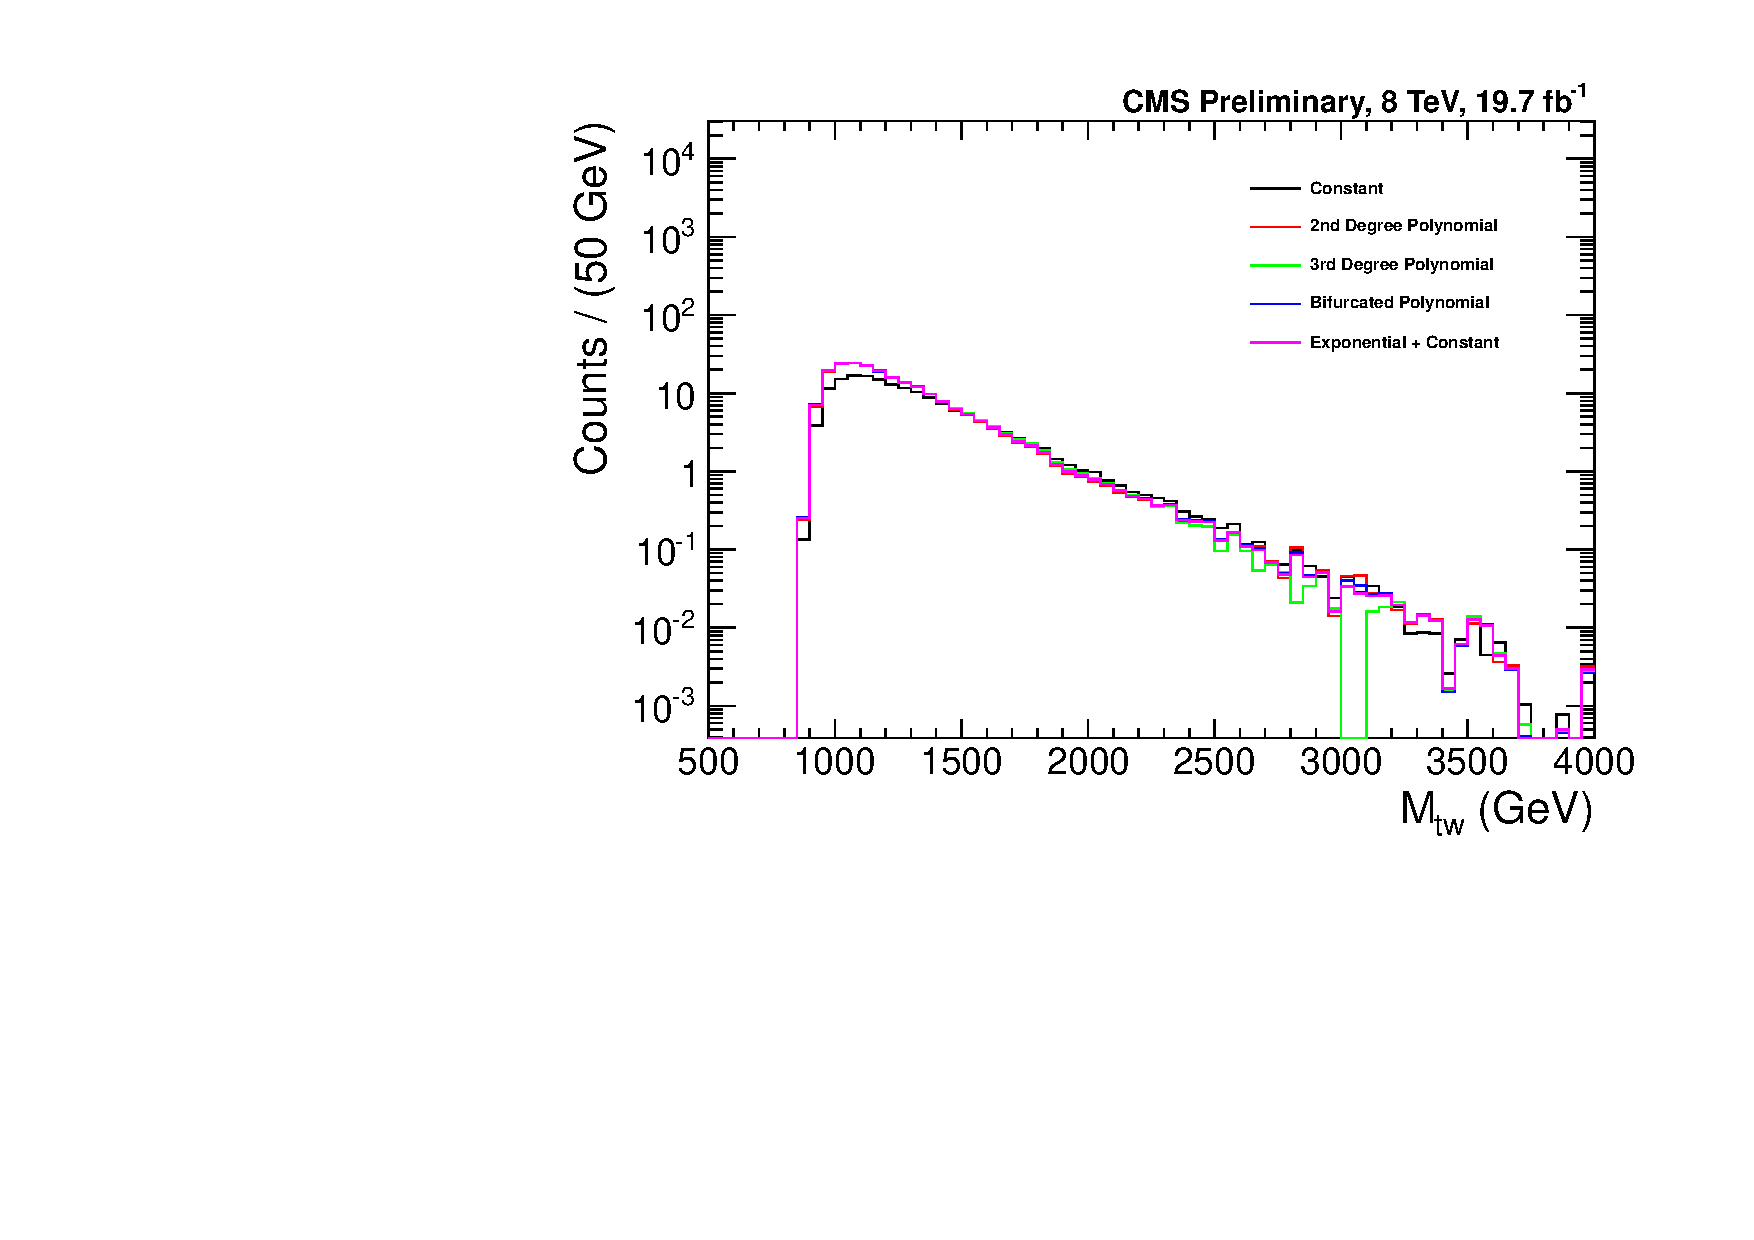
\includegraphics[width=0.7\textwidth]{AN-14-049/figs/BKGCOMPLOG.pdf}
\caption{
QCD background estimation from alternative fit functions seen in \ref{figs:bsBKGFITCOMP}. Top and bottom plots are the same but on linear and log y-axis scale.
}
\label{figs:bsBKGCOMP}
\end{center}
\end{figure}

\begin{figure}[htcb]
\begin{center}
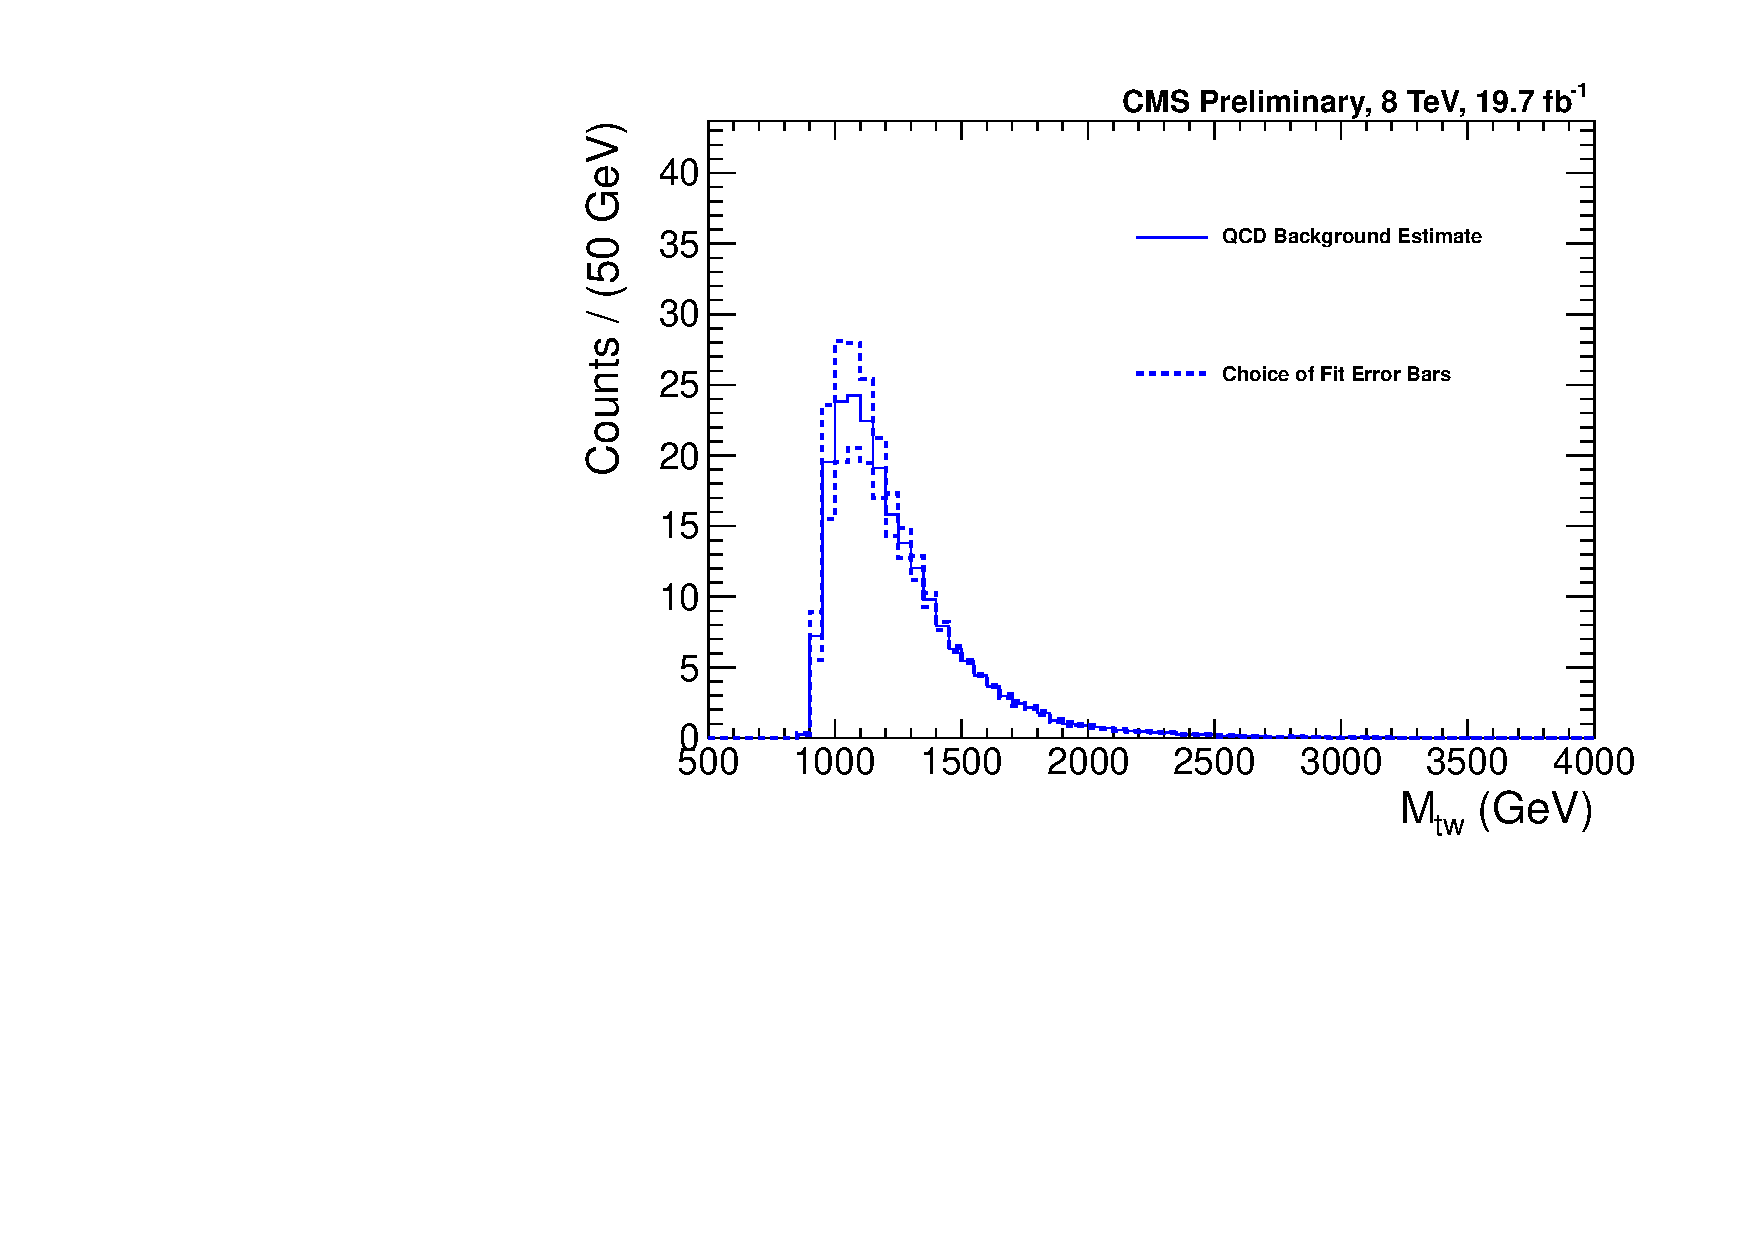
\includegraphics[width=0.7\textwidth]{AN-14-049/figs/BKGFITERR.pdf}\\
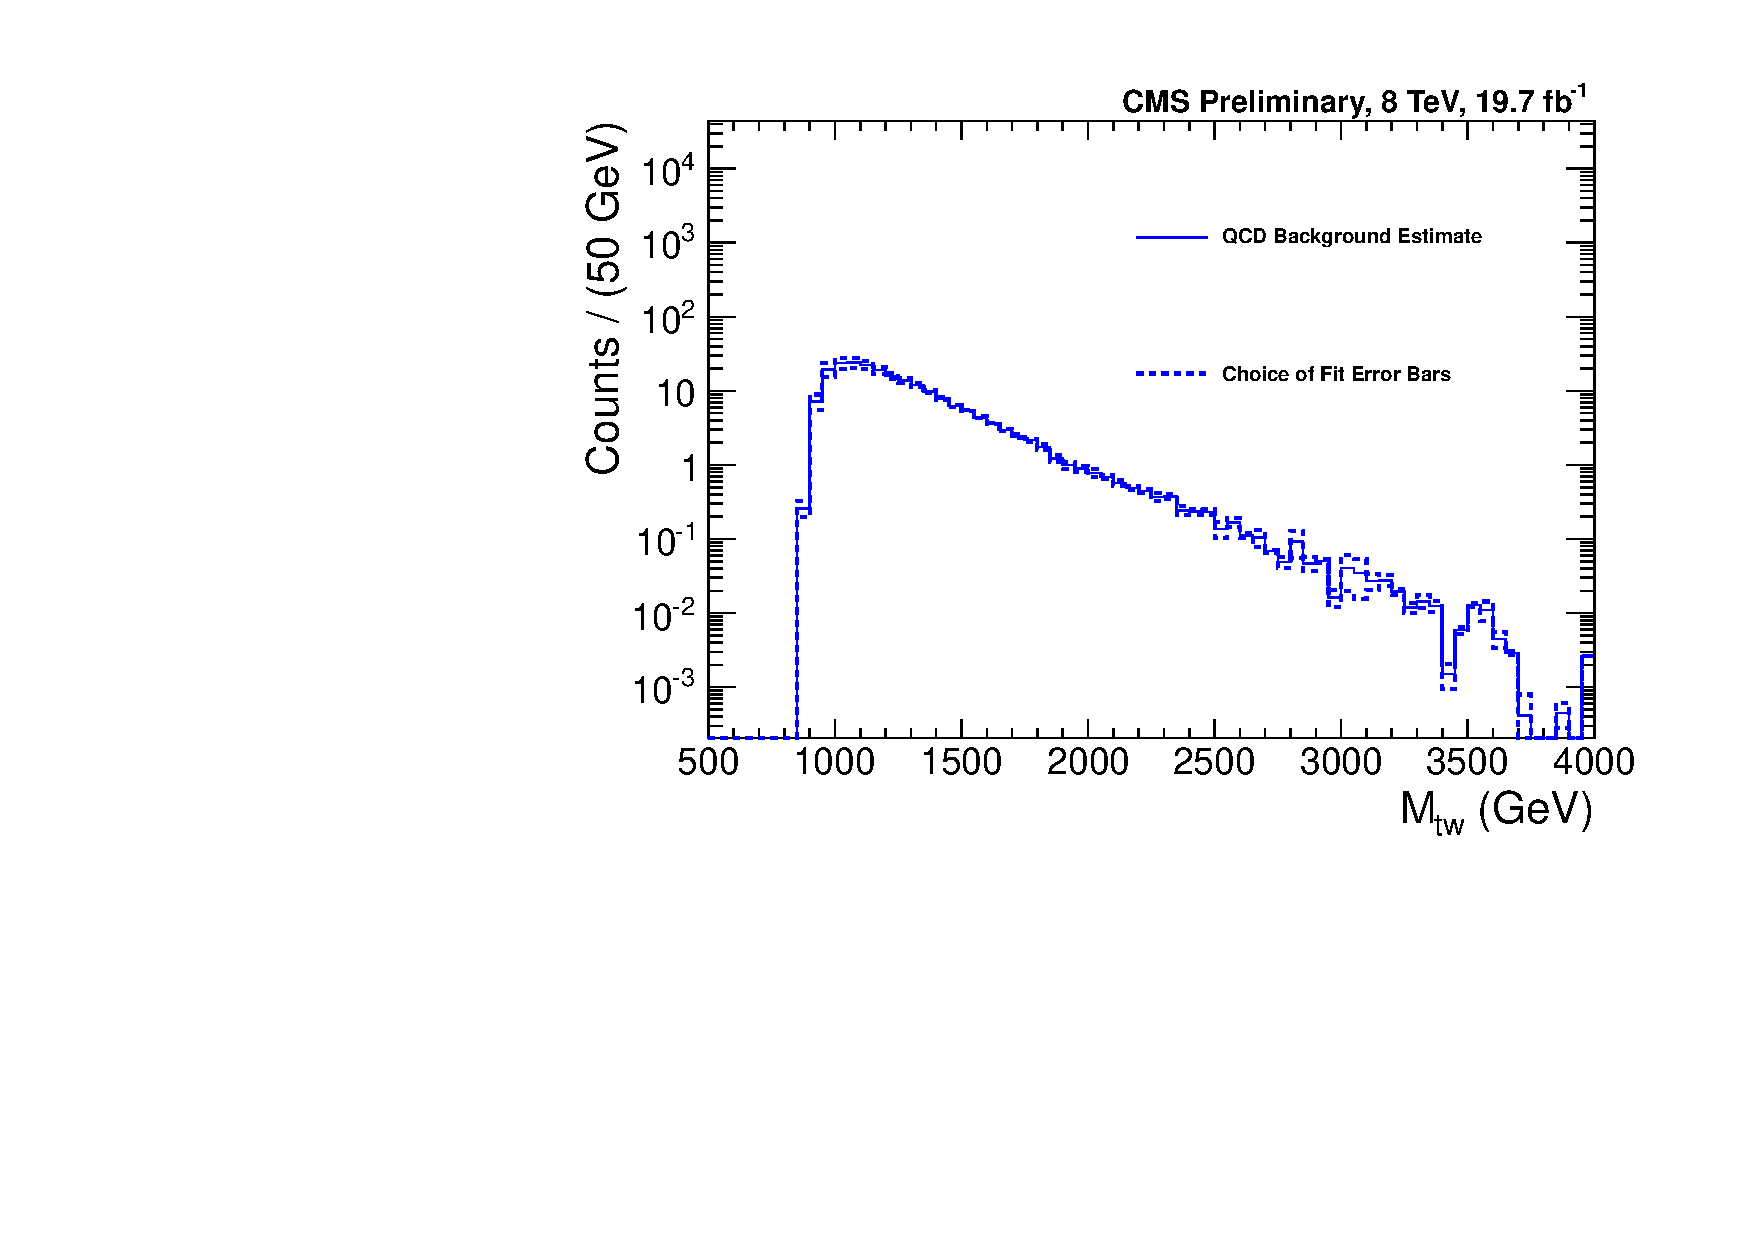
\includegraphics[width=0.7\textwidth]{AN-14-049/figs/BKGFITERRLOG.pdf}
\caption{
Uncertainty on the choice of fit as extracted from the alternative background estimations seen in \ref{figs:bsBKGCOMP}. Top and bottom plots are the same but on linear and log y-axis scale.
}
\label{figs:bsBKGERR}
\end{center}
\end{figure}

\begin{figure}[htcb]
\begin{center}
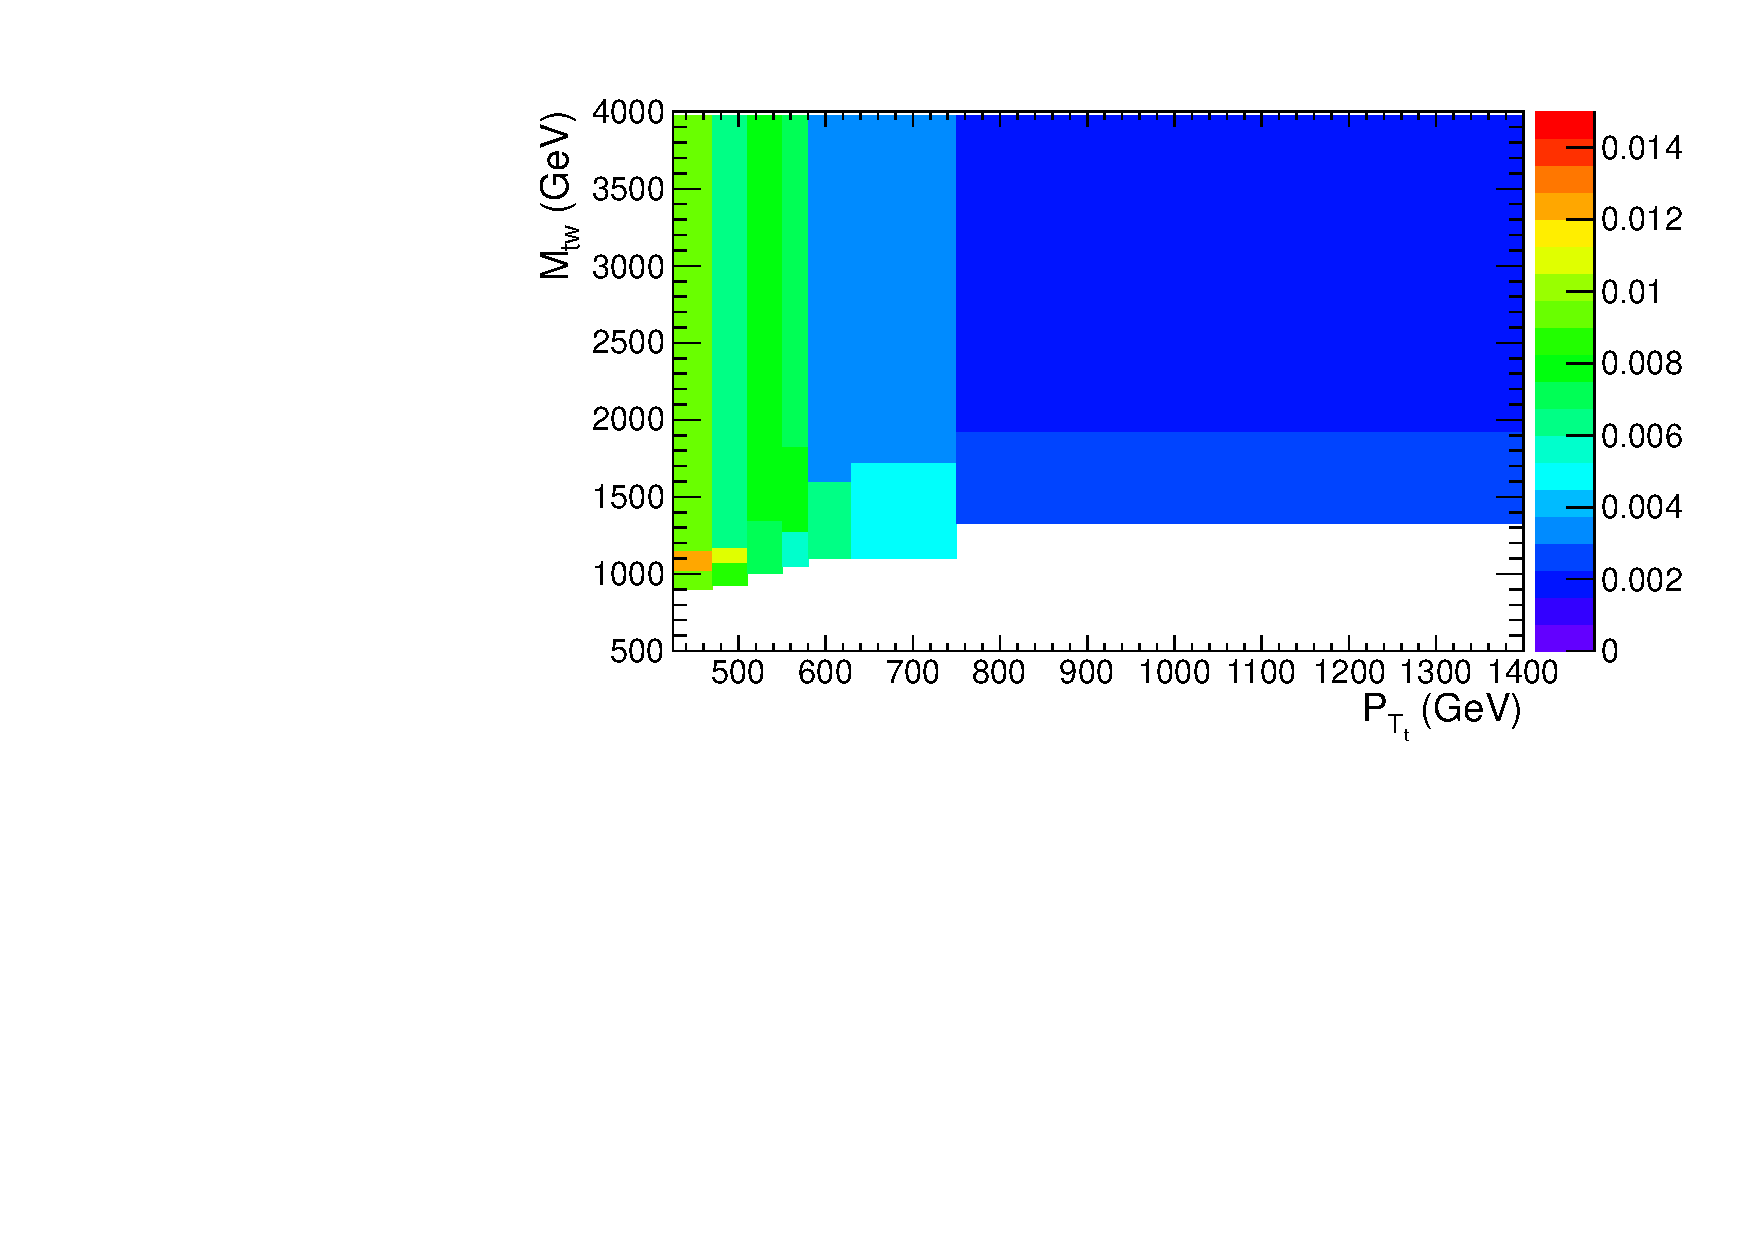
\includegraphics[width=0.7\textwidth]{AN-14-049/figs/TagrateEta1SB2dSB1.pdf}\\
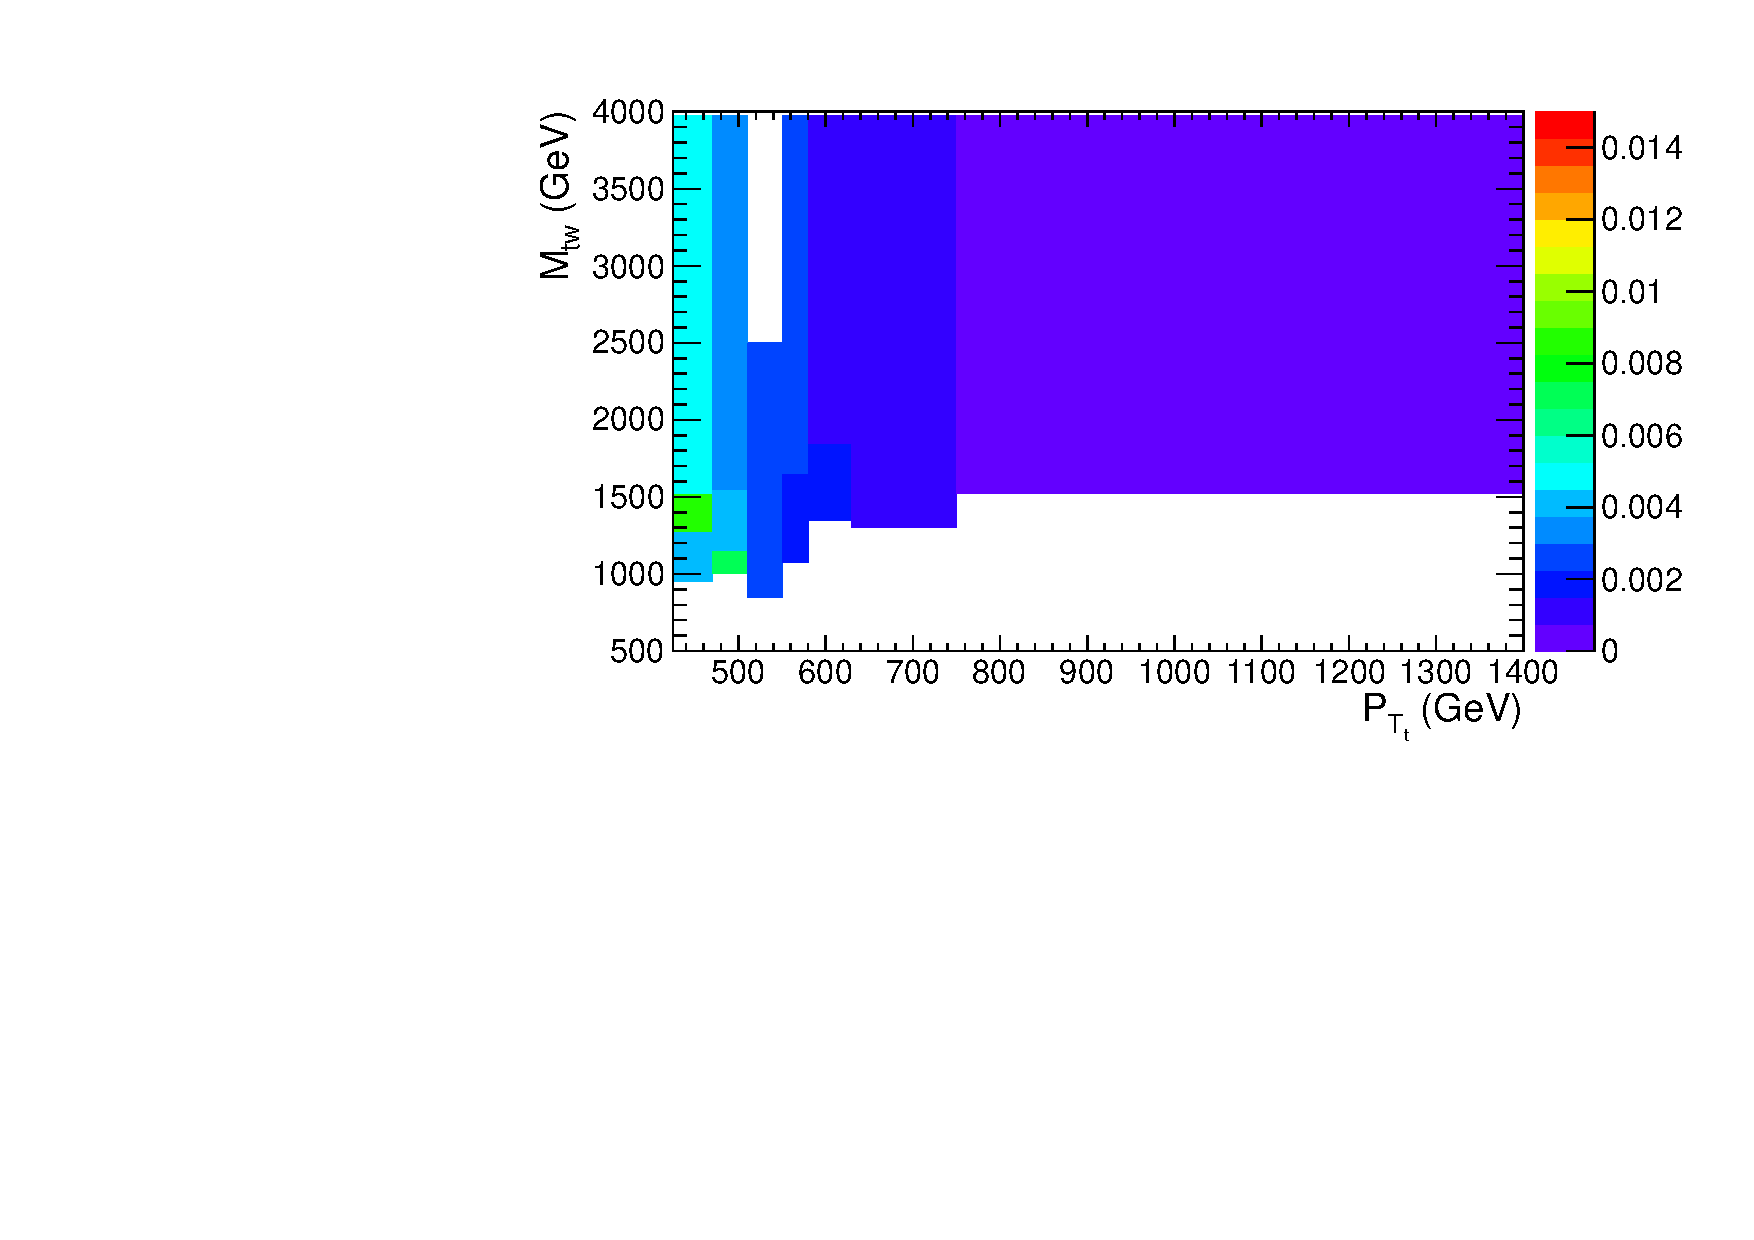
\includegraphics[width=0.7\textwidth]{AN-14-049/figs/TagrateEta2SB2dSB1.pdf}
\caption{
Two dimensional parameterization of top-mistagging rate in $\pt_{t}$ and $\mathrm{M_{tW}}$.  The x axis binning is identical to the binning in Section \ref{sec:bsbackgroundEstimation}.  
The y-axis is binned adaptively to approximate equivalent statistics over each y-axis bin per x axis bin. 
(a) Low $\eta$ Region
(b) High $\eta$ Region
}
\label{figs:bssb2deta}
\end{center}
\end{figure}

\begin{figure}[htcb]
\begin{center}
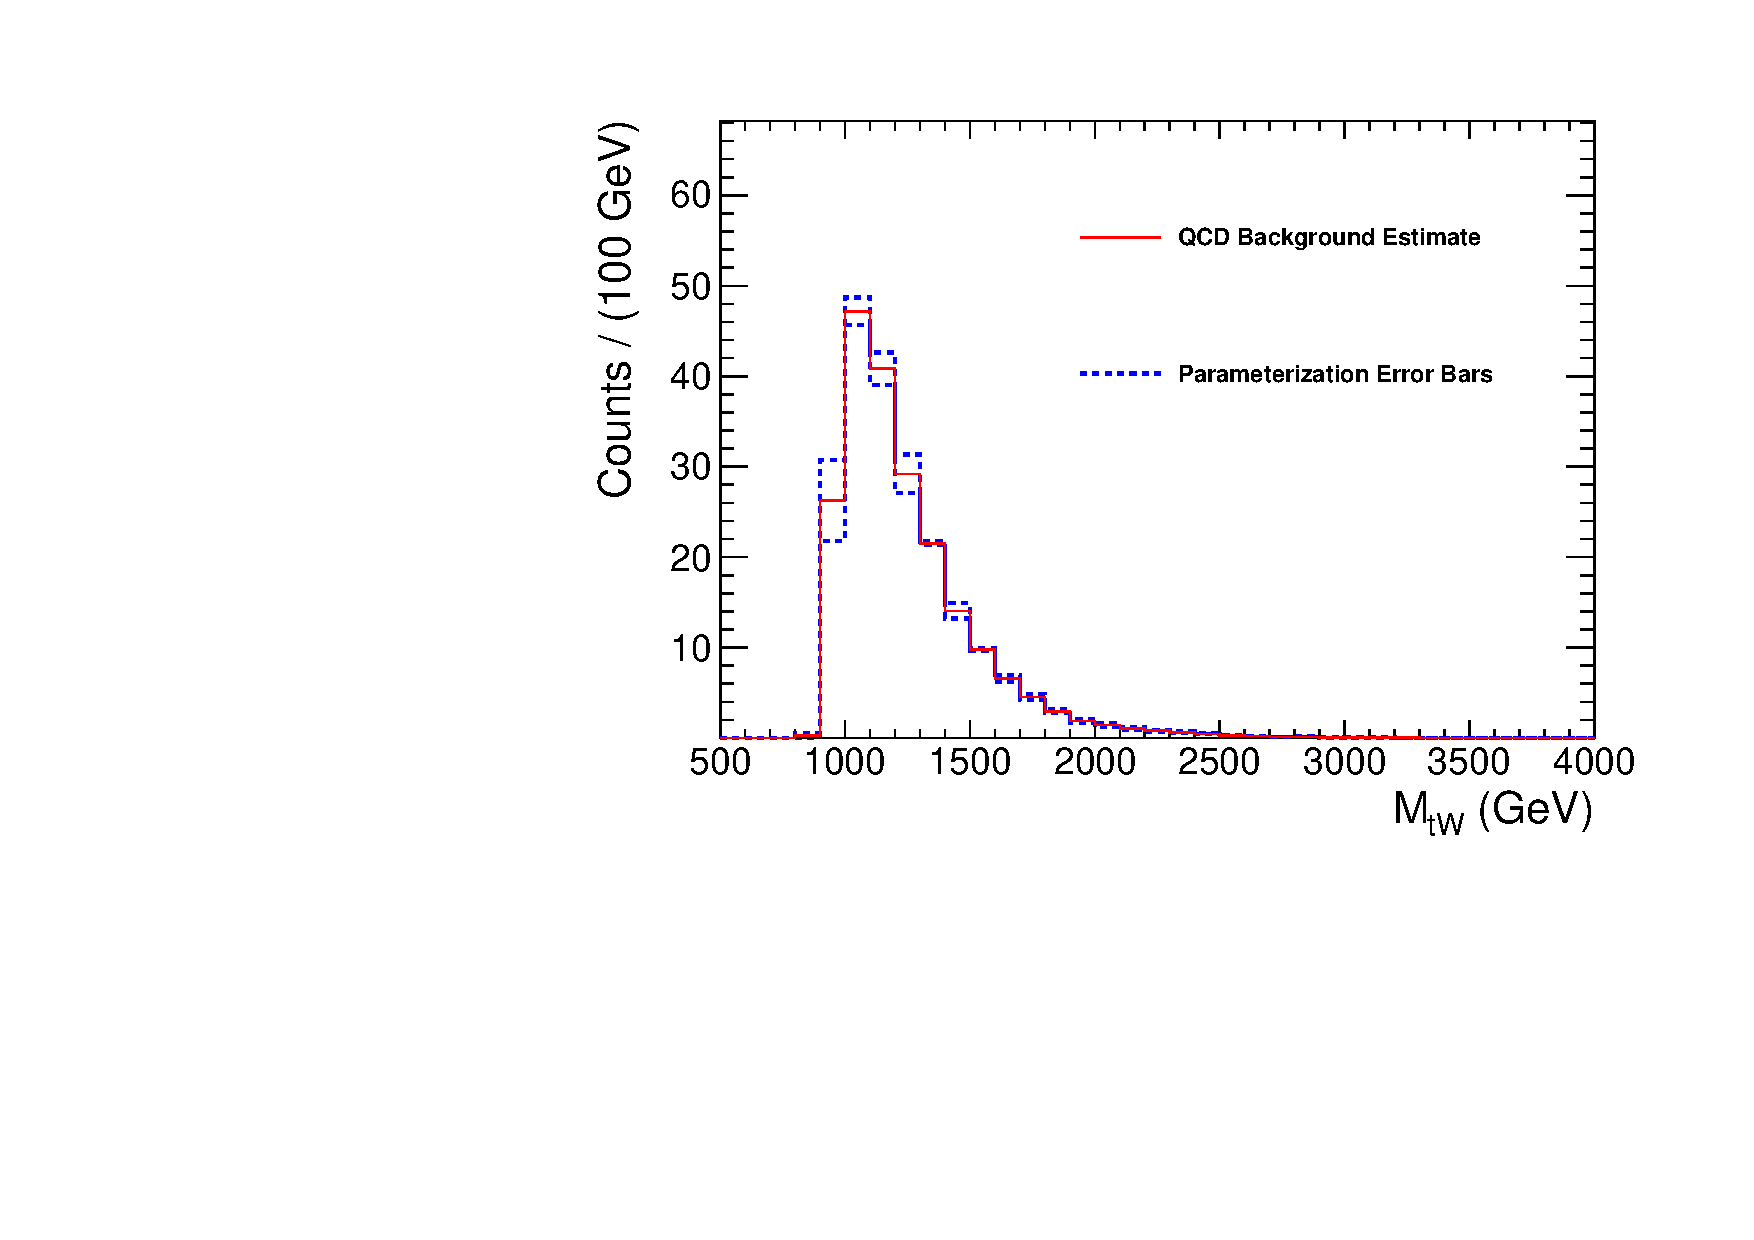
\includegraphics[width=0.7\textwidth]{AN-14-049/figs/Mtw2dvs1dBE}\\
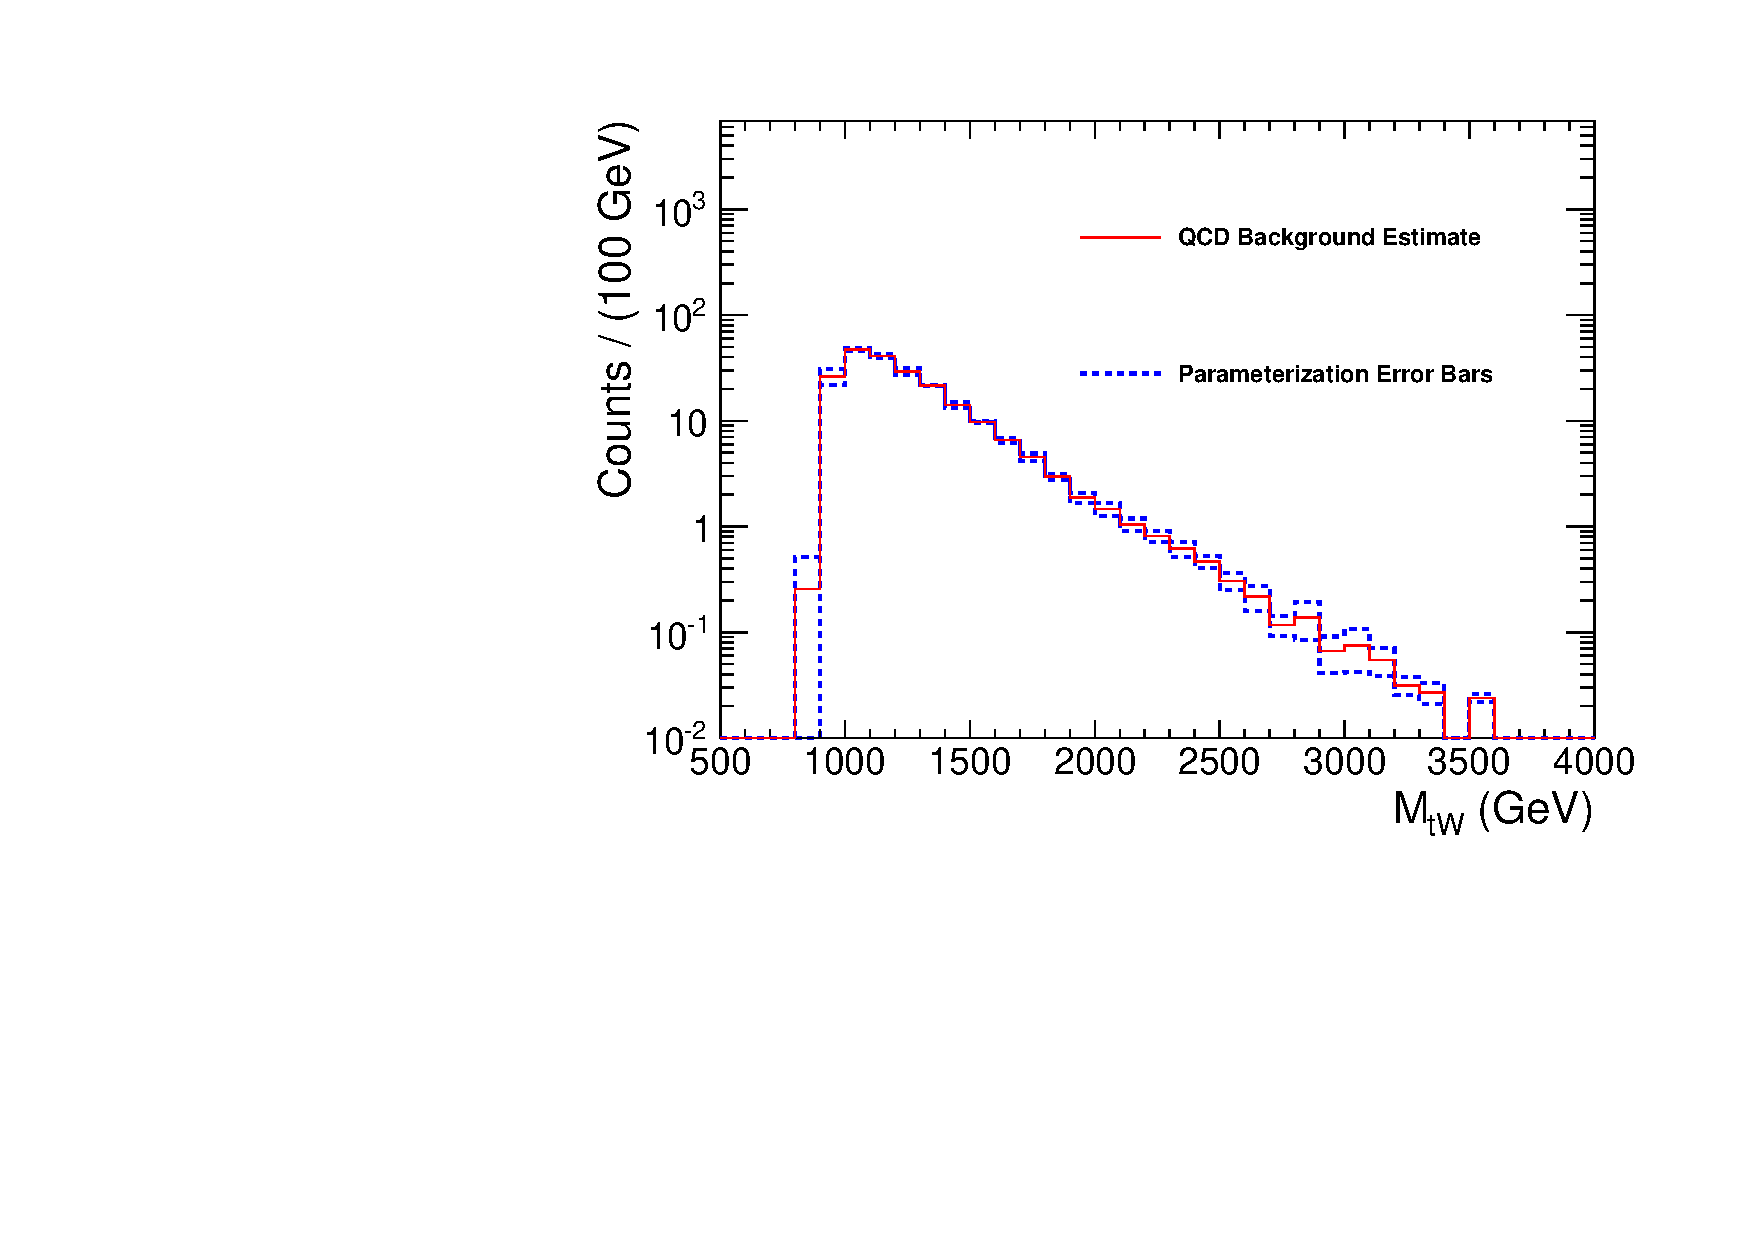
\includegraphics[width=0.7\textwidth]{AN-14-049/figs/Mtw2dvs1dBEsemilog}
\caption{
Uncertainty on the parameterization choice. Top and bottom plots are the same but on linear and log y-axis scale.
}
\label{figs:bsPARAMERROR}
\end{center}
\end{figure}

\begin{figure}[htcb]
\begin{center}
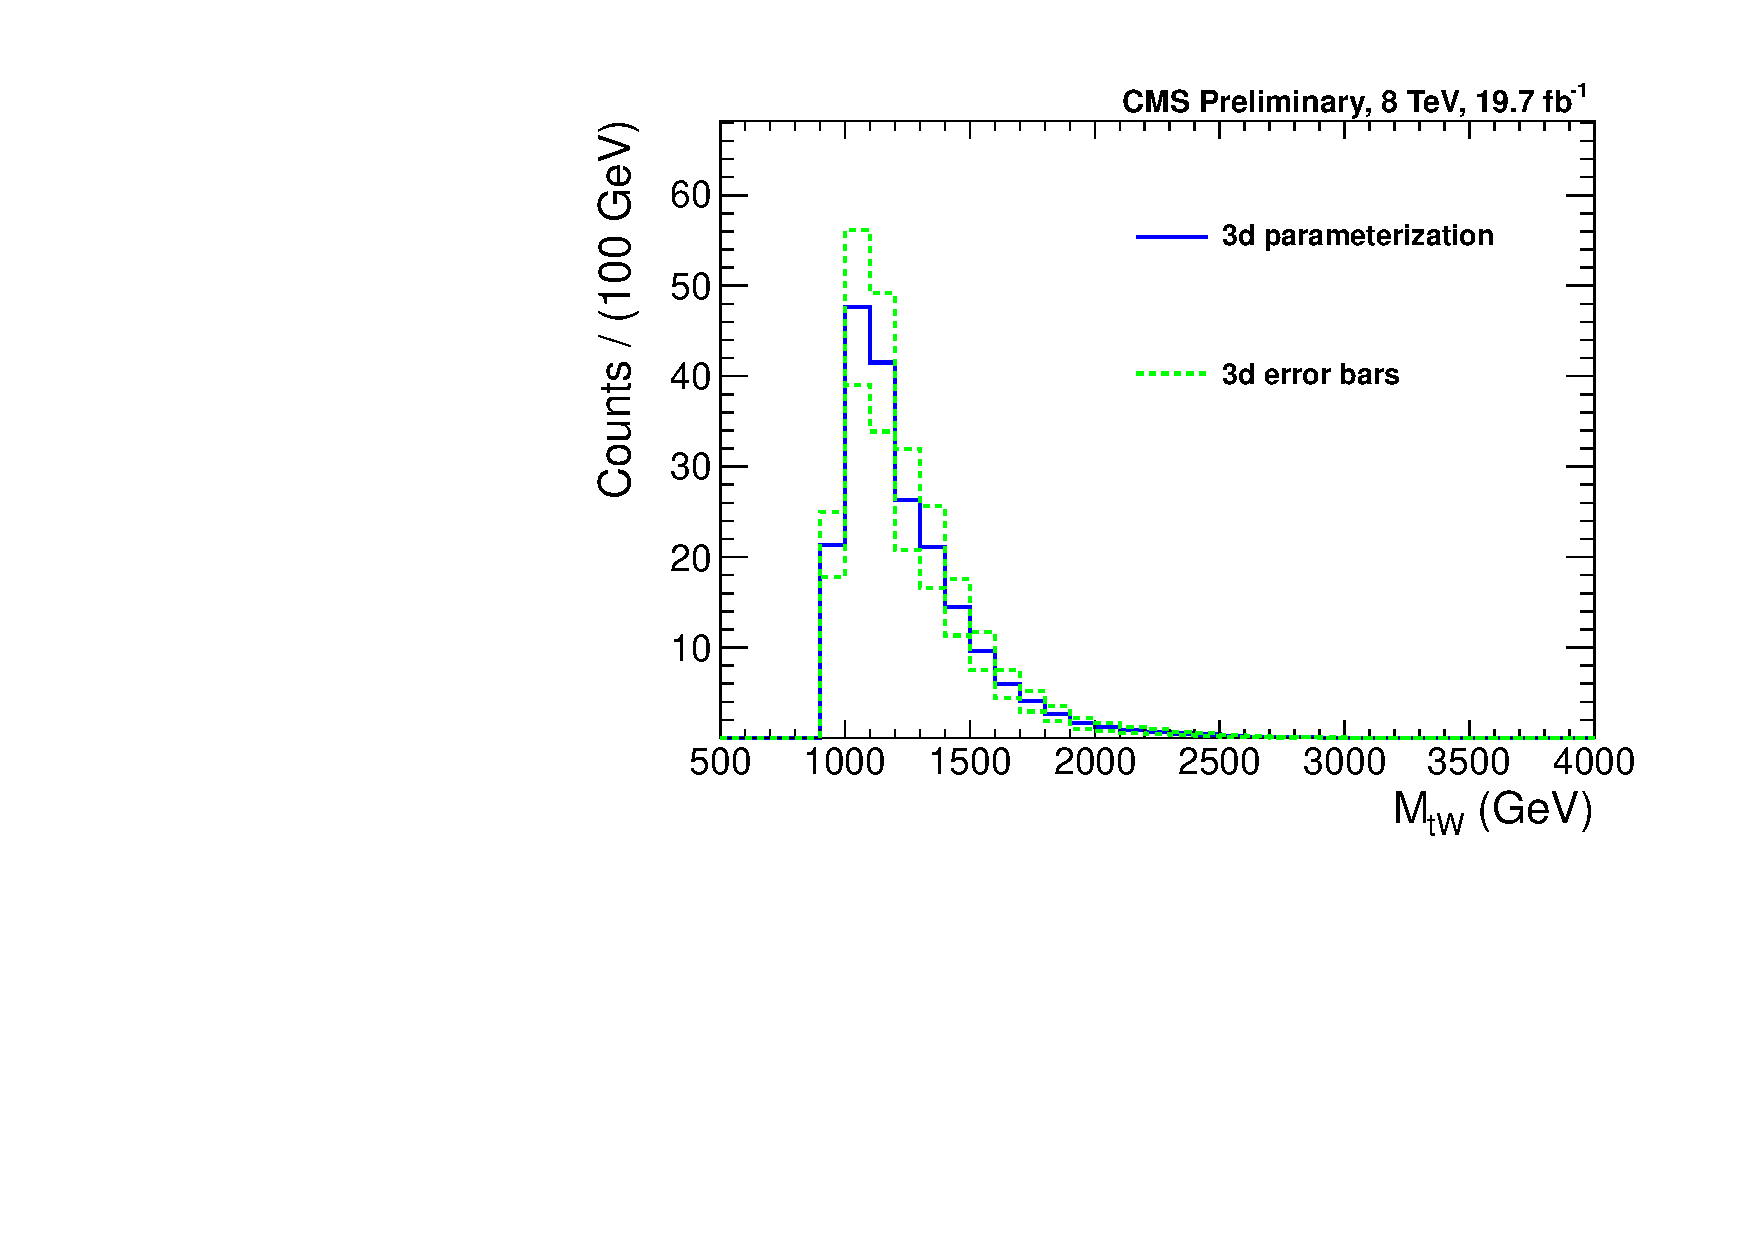
\includegraphics[width=0.7\textwidth]{AN-14-049/figs/Mtw2dstatssubtracted.pdf}
\caption{
Statistical uncertainty on the three dimensional parameterization top-mistagging rate nominal shapes.
}
\label{figs:bsPARAMERRORstat}
\end{center}
\end{figure}


